\documentclass[11pt, aps, longbibliography]{article}

%\usepackage{graphicx}% Include figure files
\usepackage{dcolumn,bm,comment}% Align table columns on decimal point
\usepackage{subfiles}
% 数式
\usepackage{amsmath,amsfonts,bm,mathcomp,physics, amssymb}
\numberwithin{equation}{section}

% 画像
\usepackage{color,float,subfigure}
\usepackage[dvipdfmx]{graphicx}
% TikZ
\usepackage{tikz}
\usetikzlibrary{intersections, calc, arrows.meta}
% 囲み
\usepackage{ascmac,fancybox}
\usepackage{tcolorbox}
\tcbuselibrary{breakable, skins, theorems}

\usepackage{listings,jvlisting} %日本語のコメントアウトをする場合jvlisting(もしくはjlisting)が必要
\usepackage[margin=30truemm]{geometry}

%\usepackage[x11names]{xcolor}
\usepackage[dvipsnames]{xcolor}
%\usepackage[colorlinks,citecolor=SpringGreen4,linkcolor=purple,dvipdfmx]{hyperref} 
\usepackage[colorlinks,citecolor=OliveGreen,linkcolor=BrickRed,dvipdfmx]{hyperref} 
\usepackage{pxjahyper}

\usepackage[backend=bibtex,style=phys,%
articletitle=false,biblabel=brackets,%
chaptertitle=false,pageranges=false]{biblatex}
\addbibresource{reference.bib}

\newtheorem{theorem}{定理}
\newtheorem{definition}{定義}
%\newtheorem{mybox}{box}
\newtcbtheorem{mybox}{My Theorem}{enhanced, %TikZの内部処理を導入する.ある程度複雑なものには必須.
    colback = white,
    colframe = green!35!black,
    fonttitle = \bfseries,
    breakable = true,
}{hoge}
\begin{document}
\title{共形場理論}
\author{Sogen Ikegami}
\date{\today}
\maketitle

\tableofcontents

\section*{preface}
\cite{yellow}に基づいて書かれた共形場理論(Conformal Field Theory, CFT)の勉強ノート.
大体のストーリーと大切だと感じたところは詳細な計算を追うことにする。
また\cite{yellow}にはないエンタングルメントとCFTの関連についても書きたい。

\newpage

\section{二次元における共形普遍性}

\subsection{二次元における共形群}
    \subsubsection{複素座標の導入}
        二次元における共形対称性を満たす変換は、複素関数における正則/反正則(holomorphic/anti-holomorphic)関数なので、
        二次元座標として複素座標を導入すると便利である。具体的には、
        \begin{align}
            z = z_0 + iz_1, &\quad  \bar{z} = z_0 - iz_1, \quad \partial_z = \frac{1}{2}(\partial_0 - i\partial_1), \quad \partial_{\bar{z}} = \frac{1}{2}(\partial_0 + i\partial_1) \\
            z_0 = \frac{1}{2}(z + \bar{z}), &\quad z_1 = \frac{1}{2i}(z-\bar{z}), \quad \partial_0 = \partial_z + \partial_{\bar{z}}, \quad \partial_0 = i(\partial_z - \partial_{\bar{z}}) 
        \end{align}
        である。また$z, \bar{z}$における計量テンソルは
        \begin{equation}
            g_{\mu\nu} = \begin{pmatrix} 0 & 1/2 \\ 1/2 & 0\end{pmatrix}, \quad g^{\mu\nu} = \begin{pmatrix} 0 & 2 \\ 2 & 0\end{pmatrix}, \quad \mu,\nu \in \left\{z, \bar{z}\right\}
        \end{equation}
        であり、正則な部分における反対称テンソルは
        \begin{equation}
            \epsilon_{\mu\nu} = \begin{pmatrix} 0 & i/2 \\ -i/2 & 0\end{pmatrix}, \quad g^{\mu\nu} = \begin{pmatrix} 0 & -2i \\ 2i & 0\end{pmatrix}, \quad \mu,\nu \in \left\{z, \bar{z}\right\}
        \end{equation}
        となる。定番の疑問が$z$と$\bar{z}$は独立か否かというものである。これに対するproperなアプローチは、
        $z_0,z_1\in \mathbb{R}$を複素値に拡張$z_0,z_1\in \mathbb{C}$することである。そうすると$z,\bar{z}$への書き換えはただの変数変換になり、
        独立な変数として扱って良いことになる。ただし、物理的に意味のある空間は$z^*=\bar{z}$を満たすような部分多様体(Real surfaceと呼ばれる)に限定する必要がある。

        \subsubsection{大域共形変換}
        共形変換の中にも、大域的に定義されているものと局所的にしか定義されないものが存在する。
        大域的に定義されている変換の集合は特殊共形群と呼ばれ、
        \begin{equation}
            f(z) = \frac{az+b}{cz+d}, \quad ad-cb=1
        \end{equation}
        で全てが尽くされる。係数を並べた行列$\begin{pmatrix} a & b \\ c & d \end{pmatrix}$とその積演算によって写像の合成ができる。determinantの値はゼロでない限りどれに取っても変わらないので単に1に置いている。
        この行列がなす群は$SL(2,\mathbb{C})$と呼ばれ、四次元のローレンツ群$SO(3,1)$に同型である。

    \subsubsection{共形変換の生成子}
        上で見た大域共形変換に拘らず、非可逆なもの(ローカルなもの)も許して共形変換の生成子がどのような代数を満たすかを見てみる。
        生成子がローラン展開できるという仮定のもと、
        \begin{equation}
            z^\prime = z + \epsilon(z), \quad \epsilon(z) = \sum_{n = -\infty}^{\infty}c_n z^{n+1}
        \end{equation}
        とおく。無限小の変換のもとで一次の範囲で$\epsilon(z)=\epsilon(z^\prime)$であり、$z=z^\prime-\epsilon(z^\prime)$とかけるため、スピンレスで無次元な場$\phi(z,\bar{z})$の変換は
        \begin{align}
            \phi^\prime(z^\prime,\bar{z}^\prime) &= \phi(z,\bar{z}) = \phi(z^\prime, \bar{z}^\prime) - \epsilon(z^\prime)\partial^\prime \phi(z^\prime, \bar{z}^\prime) - \bar{\epsilon}(\bar{z}^\prime) \bar{\partial}^\prime \phi(z^\prime, \bar{z}^\prime), 
        \end{align}
        \begin{align}
            \delta \phi = \phi^\prime(z^\prime, \bar{z}^\prime) - \phi^\prime(z, \bar{z}) &= -\epsilon(z)\partial \phi(z,\bar{z}) - \bar{\epsilon}(\bar{z})\bar{\partial}\phi(z, \bar{z}) \notag \\
            &= \sum_n c_n l_n \phi(z, \bar{z}) + \bar{c}_n \bar{l}_n \phi(z, \bar{z})
        \end{align}
        となる\footnote{$\delta \phi$の符号は定義による。}。ここで生成子
        \begin{equation}\label{eq:def-Witt-gens}
            l_n \equiv -z^{n+1}\partial, \quad \bar{l}_n \equiv -\bar{z}^{n+1}\bar{\partial}
        \end{equation}
        を定義した。これらの満たす代数は
        \begin{align}\label{eq:Witt-alg}
            &[l_n, l_m] = (n-m)l_{n+m} \notag \\
            &[\bar{l}_n, \bar{l}_m] = (n-m)\bar{l}_{n+m} \\
            &[l_n, \bar{l}_m] = 0 \notag 
        \end{align}
        となる。この代数はWitt-algebraと呼ばれる。正則と反正則部分が完全に分離されている。
        集合$\left\{l_0, l_1, l_{-1}\right\}$はWitt-algebraの部分代数になっており先ほどの大域共形変換を生成する。実際$l_{-1}=-\partial$は並進を、
        $l_0 = -z\partial$は回転とスケール変換を、$l_1=-z^2\partial$は特殊共形変換を生成する。
        Real surface($z_0, z_1 \in \mathbb{R}$)を保つような変換は
        \begin{equation}
            l_n + \bar{l}_{n}, \quad i(l_n - \bar{l}_{n})
        \end{equation}
        で生成される。特に$l_0 + \bar{l}_{0}$はdilationを生成する。のちにFree bosonでやる際には動径量子化を行うが、動径方向に時間を取るためこれがHamiltonianに対応することになる。

        \subsubsection{プライマリー場}
        スケーリング次元$\Delta$でスピン(SO(2)回転に対するチャージ)$s$であるような場を考える。正則共形次元とその反正則な部分を
        \begin{equation}
            h = \frac{1}{2}(\Delta + s), \quad \bar{h} = \frac{1}{2}(\Delta -s )
        \end{equation}
        で定義する。準プライマリー場は共形変換$z\rightarrow w(z), \bar{z}\rightarrow \bar{w}(\bar{z})$に対して
        \begin{equation}
            \phi^{\prime}(w, \bar{w}) = \left(\frac{\partial w}{\partial z}\right)^{-h} \left(\frac{\partial \bar{w}}{\partial \bar{z}}\right)^{-\bar{h}} \phi(z, \bar{z})
        \end{equation}
        と変換する。準プライマリー場とは大域的な共形変換に対して上式のように変換する場のことであり、$l_{-1}, l_0, l_1$で生成される変換の変換性による定義である。
        一方、全ての$l_n$で生成される共形変換に対して上式のように変換する場をプライマリー場と呼ぶ。定義からプライマリー場は準プライマリー場である。一方、準プライマリー場であってプライマリー場でないものはあり、
        energy momentum テンソルなどが該当する。プライマリー場でない場をセカンダリー場と呼ぶ。
        2点、3点相関関数は定数を除いて完全に決定される。4点相関関数は完全には決定されない。

    \subsection{Ward恒等式}
    \subsubsection{正則形式のWard恒等式}
        ビリアルカレントを用いて、共形対称性がある場合energy momentumテンソルを対称でトレースネスにできる(と信じられている)のであった。
        並進、回転(Lorentz変換)、拡大に対するWard恒等式\footnote{古典論では対称性に付随するNoetherカレントは常に保存する。しかし場の量子論においては、カレントオペレータと他のオペレータが同じ座標にある場合(左辺)に異常がおき、右辺のような値が出る。その関係を記述しているのがWard恒等式である。(Schwinger-Dysonなどの議論で納得できる。)}
        はそれぞれ以下のようになる。
        \begin{align}
            \frac{\partial}{\partial x^\mu} \expval{T^\mu_{\ \nu}(\bm{x})X} &= - \sum_{i=1}^{n} \delta(\bm{x}- \bm{x}_i) \frac{\partial}{\partial x_i^\nu}\expval{X} \label{eq:ward1} \\
            \epsilon_{\mu\nu}\expval{T^{\mu\nu}(\bm{x})X} &= -i \sum_{i=1}^{n}s_i \delta(\bm{x}- \bm{x}_i) \expval{X} \label{eq:ward2} \\
            \expval{T^\mu_{\ \mu}X} &= - \sum_{i=1}^{n}\delta(\bm{x}- \bm{x}_i)\Delta_i \expval{X} \label{eq:ward3}
        \end{align}
        ここで$X$は$n$個のプライマリー場のストリング$\Phi(\bm{x}_1)\cdots \Phi(\bm{x}_n)$である。
        これらを複素座標を用いて書き換える。デルタ関数について、
        \begin{equation}
            \delta(\bm{x}) = \frac{1}{\pi} \bar{\partial}\frac{1}{z} = \frac{1}{\pi} \partial \frac{1}{\bar{z}}
        \end{equation}
        が成り立つことを用いる\footnote{何らかのテスト関数に当てて積分するとテスト関数の一点の値が出てくることから確認できる。}と、例えば並進のWard恒等式は次のようになる。
        \begin{align}
            \frac{\partial}{\partial x^0} \expval{T^0_{\  0}(\bm{x})X} + \frac{\partial}{\partial x^1} \expval{T^1_{\  0}(\bm{x})X} &= - \sum_{i=1}^{n} \delta(\bm{x}- \bm{x}_i) \frac{\partial}{\partial x_i^0}\expval{X} \notag \\
            \left(  \partial + \bar{\partial}\right) \expval{T^0_{\  0}(z)X} + i\left(  \partial - \bar{\partial}\right)  \expval{T^1_{\  0}(z)X} &= -\sum_{i=1}^{n} \frac{1}{\pi} \bar{\partial} \frac{1}{z-w_i}\left(  \partial_{w_i} + \bar{\partial}_{w_i}\right) \expval{X}
        \end{align}
        \begin{align}
            \frac{\partial}{\partial x^0} \expval{T^0_{\  1}(\bm{x})X} + \frac{\partial}{\partial x^1} \expval{T^1_{\  1}(\bm{x})X} &= - \sum_{i=1}^{n} \delta(\bm{x}- \bm{x}_i) \frac{\partial}{\partial x_i^1}\expval{X} \notag \\
            \left(  \partial + \bar{\partial}\right) \expval{T^0_{\  1}(z)X} + i\left(  \partial - \bar{\partial}\right)  \expval{T^1_{\  1}(z)X} &= -i\sum_{i=1}^{n} \frac{1}{\pi} \bar{\partial} \frac{1}{z-w_i}\left(  \partial_{w_i} - \bar{\partial}_{w_i}\right) \expval{X}
        \end{align}
        二つ目の式に$-i$をかけて足すと、
        \begin{align}
            \left( \partial + \bar{\partial}\right) \expval{T^0_{\  0}(z)X} &+ \left( \partial - \bar{\partial}\right) \expval{T^1_{\ 1}(z)X} + i\left(  \partial - \bar{\partial}\right)  \expval{T^1_{\  0}(z)X} -i\left(  \partial + \bar{\partial}\right) \expval{T^0_{\  1}(z)X}  \notag \\
            &= -\sum_{i=1}^{n} \frac{2}{\pi} \bar{\partial} \frac{1}{z-w_i} \partial_{w_i} \expval{X}
        \end{align}
        エネルギー運動量テンソルのトレースレスな関係$T^\mu_\mu = 0$と対称性$T^\mu_\nu = T^\nu_\mu$を用いると、
        \begin{equation}\label{eq:ward-trans-1}
            \partial\expval{\left(T^0_{\  0}+T^1_{\  1}\right)X}  + \bar{\partial} \expval{\left(T^0_{\ 0}-2iT^1_{\  0}-T^1_{\ 1}\right)X} = - \sum_{i=1}^{n} \frac{2}{\pi} \bar{\partial} \frac{1}{z-w_i} \partial_{w_i}\expval{X}
        \end{equation}
        ここで、テンソルの添え字の変換則
        \begin{equation}
            T_{zz} = \frac{\partial x^\mu}{\partial z}\frac{\partial x^\nu}{\partial z} T_{\mu\nu}
        \end{equation}
        を用いると、式\eqref{eq:ward-trans-1}は
        \begin{equation}\label{eq:ward-trans-2}
            2\pi \partial \expval{T_{\bar{z}z}X} + 2\pi \bar{\partial} \expval{T_{zz}X} = - \sum_{i=1}^{n} \bar{\partial} \frac{1}{z-w_i} \partial_{w_i} \expval{X}
        \end{equation}
        となる。他の関係式は次のようになる。
        \begin{align}
            2\pi \partial \expval{T_{\bar{z}\bar{z}}X} + 2\pi \bar{\partial} \expval{T_{z\bar{z}}X} &= - \sum_{i=1}^{n} \partial \frac{1}{\bar{z}-\bar{w}_i}  \partial_{\bar{w}_i} \expval{X} \label{eq:ward-trans-3} \\
            2 \expval{T_{z\bar{z}}X} + 2\expval{T_{\bar{z}z}X} &= - \sum_{i=1}^{n} \delta(\bm{x}-\bm{x}_i) \Delta_i \expval{X} \\
            -2 \expval{T_{z\bar{z}}X} + 2\expval{T_{\bar{z}z}X} &= - \sum_{i=1}^{n} \delta(\bm{x}-\bm{x}_i) s_i \expval{X} 
        \end{align}
        最後の二式を足し引きすると、
        \begin{align}
            2\pi \expval{T_{\bar{z}z}X} &= - \sum_{i=1}^{n} \partial_{\bar{z}} \frac{1}{z-w_i} h_i \expval{X} \label{eq:ward-1} \\
            2\pi \expval{T_{z\bar{z}}X} &= - \sum_{i=1}^{n} \partial_{z} \frac{1}{\bar{z}-\bar{w}_i} \bar{h}_i \expval{X} \label{eq:ward-2}
        \end{align}
        式\eqref{eq:ward-1}\eqref{eq:ward-2}を式\eqref{eq:ward-trans-2}\eqref{eq:ward-trans-3}に代入して、次式を得る。
        \begin{align}
            \partial_{\bar{z}}\left\{ \expval{T(z,\bar{z})X} - \sum_{i=1}^{n} \left[ \frac{1}{z-w_i}\partial_{w_i}\expval{X} + \frac{h_i}{(z-w_i)^2}\expval{X} \right] \right\} &= 0 \label{eq:tx1} \\
            \partial_{z}\left\{ \expval{\bar{T}(z,\bar{z})X} - \sum_{i=1}^{n} \left[ \frac{1}{\bar{z}-\bar{w}_i}\partial_{\bar{w}_i}\expval{X} + \frac{\bar{h}_i}{(\bar{z}-\bar{w}_i)^2}\expval{X} \right] \right\} &= 0 \label{eq:tx2}
        \end{align}
        ここで、
        \begin{equation}\label{eq:def-T}
            T(z,\bar{z}) = -2\pi T_{zz}, \quad \bar{T}(z,\bar{z}) = -2\pi T_{\bar{z}\bar{z}}
        \end{equation}
        と定義した。

    \subsubsection{共形Ward恒等式}
        三つのWard恒等式\eqref{eq:ward1}\eqref{eq:ward2}\eqref{eq:ward3}を一つの形にまとめることもできる。任意の共形変換$\epsilon^\nu(\bm{x})$において、
        \begin{align}
            \partial_\mu(\epsilon_\nu T^{\mu\nu}) &= \epsilon_{\nu}\partial_\mu T^{\mu\nu} + \frac{1}{2}(\partial_\mu \epsilon_\nu + \partial_\nu \epsilon_\mu)T^{\mu\nu} + \frac{1}{2}(\partial_\mu \epsilon_\nu - \partial_\nu \epsilon_\mu)T^{\mu\nu} \notag \\
            &= \epsilon_{\nu}\partial_\mu T^{\mu\nu} + \frac{1}{2}(\partial_\rho \epsilon^{\rho})\eta_{\mu\nu}T^{\mu\nu} + \frac{1}{2}\epsilon^{\alpha\beta}\partial_\alpha \epsilon_\beta \epsilon_{\mu\nu}T^{\mu\nu} 
        \end{align}
        両辺に$X$を当てて$X$の全ての点を含む領域$M$で積分すると、右辺は共形変換による$X$の変化分になるので、
        \begin{equation}
            \delta_\epsilon \expval{X} = \int_M d^2x \ \partial_\mu \expval{T^{\mu\nu}(\bm{x})\epsilon_\nu(\bm{x})X}
        \end{equation}
        が得られる。Gaussの定理$\int_M d^2x \ \partial_\mu F^\mu = \int_{\partial M}d\xi_\mu F^\mu$
        を適用できる。ここで、$d\xi$は$M$の境界に垂直な向きにある。これを$\partial M$の反時計回りの経路積分$d\xi_\mu = \epsilon_{\mu\rho}ds^\rho$を使うと便利である。というのも、
        複素座標において$ds$の正則(反正則)な部分は$dz, d\bar{z}$になり、
        \begin{align}
            \int_M d^2x \ \partial_\mu F^\mu &= \int_{\partial M} \left[ dz \ \epsilon_{\bar{z}z}F^{\bar{z}} + d\bar{z} \ \epsilon_{z\bar{z}}F^z \right] \notag \\
            &= \frac{i}{2} \int_{\partial M} \left[ -dz \ F^{\bar{z}} + d\bar{z} \ F^z \right]
        \end{align}
        とできる。ここに$F^\mu = \expval{T^{\mu\nu}(\bm{x})\epsilon_\nu(\bm{x})X}$を代入すると、
        \begin{equation}
            \delta_{\epsilon, \bar{\epsilon}}\expval{X} = \frac{i}{2}\int_C \left[ -dz \ \expval{T^{\bar{z}\bar{z}}\epsilon_{\bar{z}}X} + d\bar{z} \ \expval{T^{zz}\epsilon_z X} \right]
        \end{equation}
        積分経路は$X$の$n$点を通らないことから、$\expval{T_{z\bar{z}}X}$などは積分に寄与しない。\eqref{eq:def-T}を代入して、以下の共形Ward恒等式を得る。
        \begin{equation}\label{eq:conformal-ward}
            \delta_{\epsilon,\bar{\epsilon}}\expval{X} = -\frac{1}{2\pi i}\oint_C dz \ \epsilon(z)\expval{T(z)X} + \frac{1}{2\pi i}\oint_C d\bar{z} \ \bar{\epsilon}(\bar{z})\expval{\bar{T}(\bar{z})X}
        \end{equation}
        これが本節の主結果である。
        出発点のWard恒等式を通してプライマリー場の性質を使って導出されたが、この関係式はプライマリー場でなくても成り立ち、相関関数内における局所場の任意の共形変換の定義と考えることもできる。
        この式を大域共形変換に適用してやると$SL(2,\mathbb{C})$の変換が導出されるほか、相関関数の形がかなり制限されることもわかる。

    \subsection{自由場と演算子積展開}
        場の量子論では複数の場が同一座標にくると真空期待値などが発散してしまう。これを回避する正則化の手法に正規順序積などがある。
        演算子積展開(Operator Product Expansion, OPE)は二つの場の積を一つの正則な場(演算子)と同一座標で発散する展開係数(関数)で展開する
        手法である。これは短距離の情報を切り離して取り出している点で重要である。電磁気における多極子展開と同様の精神と考えて良い。

        エネルギー運動量テンソルとプライマリー場の演算子積展開は式\eqref{eq:tx1}からブラケットを取り除き得ることができる。
        共形次元$h,\bar{h}$のプライマリー場$\phi$に対して
        \begin{align}
            T(z)\phi(w,\bar{w}) &\sim \frac{h}{(z-w)^2}\phi(w,\bar{w}) + \frac{1}{z-w}\partial_w \phi(w,\bar{w}) \label{eq:OPE1} \\
            \bar{T}(\bar{z})\phi(w,\bar{w}) &\sim \frac{\bar{h}}{(\bar{z}-\bar{w})^2}\phi(w,\bar{w}) + \frac{1}{\bar{z}-\bar{w}}\partial_{\bar{w}} \phi(w,\bar{w})\label{eq:OPE2}
        \end{align}
        演算子積展開における$\sim$は$w\rightarrow z$における正則な項を含んでいることを意味する。エネルギー運動量テンソルとプライマリー場に関する演算子積展開も
        共形Ward恒等式からは得られない正則な寄与が無限に存在する。
        一般的に二つの場$A(z),B(w)$の演算子積展開を
        \begin{equation}\label{eq:OPE1}
            A(z)B(w) = \sum_{n=-\infty}^{N} \frac{\left\{ AB \right\}_n(w)}{(z-w)^n}
        \end{equation}
        とかく。場$\left\{ AB \right\}_n(w)$は$w=z$で特異点となっていない。例えば$\left\{ T\phi \right\}_1(w)=\partial_w \phi(w)$である。

    \subsubsection{Free Boson}
        最もシンプルな共形場理論として、質量0のボソンを考える。
        \begin{equation}\label{eq:free-boson1}
            S = \frac{1}{2}g \int d^2x \ \partial_\mu \varphi \partial^\mu \varphi
        \end{equation}
        2点関数は
        \begin{equation}\label{eq:free-boson2}
            \expval{\varphi(\bm{x})\varphi(\bm{y})} = -\frac{1}{4\pi g} \ln (\bm{x}-\bm{y})^2 + \text{const.}
        \end{equation}
        である。複素座標では
        \begin{equation}\label{eq:free-boson3}
            \expval{\varphi(z,\bar{z})\varphi(w,\bar{w})} = -\frac{1}{4\pi g}\left[ \ln(z-w) + \ln(\bar{z}-\bar{w}) \right]+ \text{const.}
        \end{equation}
        となる。正則/反正則な部分は微分を通して分離できる。
        \begin{align}\label{eq:free-boson4}
            \expval{\partial_z \varphi(z,\bar{z})\partial_w\varphi(w,\bar{w})} &= -\frac{1}{4\pi g}\frac{1}{(z-w)^2} \\
            \expval{\partial_{\bar{z}} \varphi(z,\bar{z})\partial_{\bar{w}}\varphi(w,\bar{w})} &= -\frac{1}{4\pi g}\frac{1}{(\bar{z}-\bar{w})^2}
        \end{align}
        正則な部分に注目すると、$\partial \varphi$とそれ自身の演算子積展開は
        \begin{equation}\label{eq:free-boson5}
            \partial \varphi(z) \partial\varphi(w) \sim -\frac{1}{4\pi g}\frac{1}{(z-w)^2}
        \end{equation}
        となる。これは座標の入れ替えについて対称である。エネルギー運動量テンソルは
        \begin{equation}\label{eq:free-boson6}
            T_{\mu\nu} = g\left( \partial_\mu \varphi \partial_\nu \varphi - \frac{1}{2}\eta_{\mu\nu}\partial_\rho \varphi \partial^\rho \varphi \right)
        \end{equation}
        である。複素座標における量子論では
        \begin{equation}\label{eq:free-boson7}
            T = -2\pi T_{zz} = -2\pi g : \partial \varphi \partial \varphi: 
        \end{equation}
        $::$は真空期待値が消えるように必要な正規順序積である。より正確には
        \begin{equation}\label{eq:free-boson8}
            T(z) = -2\pi g \lim_{w\rightarrow z} \left( \partial\varphi(z) \partial\varphi(w) - \expval{\partial \varphi(z)\partial\varphi(w)} \right)
        \end{equation}
        である。またエネルギー運動量テンソルと$\partial \varphi$の演算子積展開はWickの定理から計算でき、
        \begin{equation}\label{eq:free-boson9}
            T(z)\partial \varphi(w) \sim \frac{\partial \varphi(z)}{(z-w)^2}
        \end{equation}
        となる。$\partial \varphi(z)$を$w$の周りで展開して求める演算子積展開
        \begin{equation}\label{eq:free-boson10}
            T(z)\partial \varphi(w) \sim \frac{\partial \varphi(w)}{(z-w)^2} + \frac{\partial^2_w \varphi(w)}{(z-w)}
        \end{equation}
        を得る。式\eqref{eq:OPE1}と見比べると、これは$\partial \varphi$が共形次元$h=1$のプライマリー場であることを示している。
        Wickの定理により、エネルギー運動量テンソルとそれ自身の演算子積展開も計算できる。
        \begin{align}
            T(z)T(w) &= 4\pi^2 g^2 :\partial \varphi(z)\partial \varphi(z)::\partial \varphi(w) \partial \varphi(w): \notag \\
            &\sim \frac{1/2}{(z-w)^4}-\frac{4\pi g:\partial \varphi(z)\partial \varphi(w):}{(z-w)^2} \notag \\
            &\sim \frac{1/2}{(z-w)^4} + \frac{2T(w)}{(z-w)^2} + \frac{\partial T(w)}{(z-w)}
        \end{align}
        二行目最初の項は二個縮約をとったもので、第二項が一個縮約をとったものが4パターン出てきたものである。
        式\eqref{eq:OPE1}と見比べるとエネルギー運動量テンソルは正確にはプライマリー場ではない。というのも最初の項$\frac{1/2}{(z-w)^4}$があるからである。

    \subsubsection{Free Fermion}
        二次元のMajoranaフェルミオンのユークリッド作用は
        \begin{equation}\label{eq:FreeFermion1}
            S = \frac{g}{2}\int d^2x \ \Psi^\dagger \gamma^0 \gamma^\mu \partial_\mu \Psi
        \end{equation}
        $\gamma$はDirac行列でDirac代数を満たす:
        \begin{equation}\label{eq:FreeFermion2}
            \gamma^\mu \gamma^\nu + \gamma^\nu \gamma^\mu = 2\eta^{\mu\nu}
        \end{equation}
        $\eta^{\mu\nu} = \text{diag}(1,1)$のとき、$\gamma$行列の表現は
        \begin{equation}\label{eq:FreeFermion3}
                \gamma^0 = \begin{pmatrix}0 & 1 \\ 1 & 0\end{pmatrix}, \quad \gamma^1 =  \begin{pmatrix}0 & -i \\ i & 0\end{pmatrix}
        \end{equation}
        したがって
        \begin{equation}\label{eq:FreeFermion4}
            \gamma^0 (\gamma^0 \partial_0 + \gamma^1 \partial_1) = 2 \begin{pmatrix}\partial_{\bar{z}} & 0 \\ 0 & \partial_z \end{pmatrix}
        \end{equation}
        two-componentのスピノル$\Psi$を$(\psi, \bar{\psi})$で書くと、作用は
        \begin{equation}\label{eq:FreeFermion5}
            S = g\int d^2x \ \left( \bar{\psi}\partial \bar{\psi} + \psi \bar{\partial} \psi \right)
        \end{equation}
        で、古典的な運動方程式は$\partial \bar{\psi}=0$と$\bar{\partial}\psi = 0$であり、解は正則/反正則な関数$\psi(z),\bar{\psi}(\bar{z})$となる。
        2点相関関数はグラスマン数のガウシアン積分に関する知見から計算できて、複素座標で
        \begin{align}\label{eq:FreeFermion6}
            \expval{\psi(z, \bar{z})\psi(w, \bar{w})} &= \frac{1}{2\pi g}\frac{1}{z-w} \\
            \expval{\bar{\psi}(z, \bar{z})\bar{\psi}(w, \bar{w})} &= \frac{1}{2\pi g}\frac{1}{\bar{z}-\bar{w}} \\
            \expval{\psi(z, \bar{z})\bar{\psi}(w, \bar{w})} &= 0
        \end{align}
        と導出される。また、
        \begin{align}\label{eq:FreeFermion7}
            \expval{\partial_z \psi(z,\bar{z})\psi(w,\bar{w})} = -\frac{1}{2\pi g}\frac{1}{(z-w)^2} \\
            \expval{\partial_z \psi(z, \bar{z})\partial_w\psi (w, \bar{w})} = -\frac{1}{\pi g}\frac{1}{(z-w)^3}
        \end{align}
        などがわかり、フェルミオン同士の演算子展開は
        \begin{equation}\label{eq:FreeFermion8}
            \psi(z)\psi(w) \sim \frac{1}{2\pi g}\frac{1}{z-w}
        \end{equation}
        となる。しっかり反交換するようになっている。エネルギー運動量テンソルは定義に従って計算すると
        \begin{equation}\label{eq:FreeFermion9}
            T(z) = -\pi g :\psi(z)\partial \psi(z):
        \end{equation}
        であり、フェルミオン場との演算子積展開は
        \begin{align}\label{eq:FreeFermion10}
            T(z)\psi(w) &= -\pi g:\psi(z)\partial \psi(z): \psi(w) \notag \\
            &\sim \frac{1}{2}\frac{\partial \psi(z)}{(z-w)} + \frac{1}{2}\frac{\psi(z)}{(z-w)^2} \notag \\
            &\sim \frac{1}{2}\frac{\psi(w)}{(z-w)^2} + \frac{1}{2}\frac{\partial \psi(w)}{(z-w)}
        \end{align}
        式\eqref{eq:OPE1}と見比べて、フリーフェルミオンは共形次元が$h=1/2$であることがわかる。エネルギー運動量テンソル自身の演算子積展開は
        \begin{align}\label{eq:FreeFermion11}
            T(z)T(w) &= \pi^2 g^2 :\psi(z)\partial\psi(z)::\psi(w)\partial\psi(w): \notag \\
            &\sim \left( \frac{1}{2} - \frac{1}{4} \right) \frac{1}{(z-w)^4} + \frac{2T(w)}{(z-w)^2} + \frac{\partial T(w)}{z-w}
        \end{align}
        従って、bosonと最初の異常項(anomalous term)の係数以外は同じである。

    \subsection{中心電荷}
        前節までの結果から、エネルギー運動量テンソル同士の演算子展開は次のような形をしている。
        \begin{equation}\label{eq:centralcharge1}
            T(z)T(w) \sim \frac{c/2}{(z-w)^4} + \frac{2T(w)}{(z-w)^2} + \frac{\partial T(w)}{(z-w)}
        \end{equation}
        ここで$c$は中心電荷(central charge)と呼ばれる量で、Free boson で$c=1$、free fermionで$c=1/2$である。この量は系の対称性などからは決められず、理論の短距離での振る舞いで決定される。
        自由場の場合エネルギー運動量テンソルとWickの定理から導出された。二つの自由場がdecoupleしてある場合、エネルギー運動量テンソルは単に二つの場のテンソルの和となり、それに従って
        中心電荷も二つの場の中心電荷の和となる。このことからナイーブには中心電荷は理論が持つ自由度の和となっている。

        中心電荷は共形異常(conformal anomaly)とも言われ、系にマクロな長さスケールを導入した際の共形対称性の"ソフトな"破れを表している。例えば系の境界条件を変更した際などがそれにあたる。
        その例として、複素平面上の理論をシリンダーにマップしてみよう。
        \begin{equation}\label{eq:centralcharge2}
            z \rightarrow w = \frac{L}{2\pi} \ln z
        \end{equation}
        すると、エネルギー運動量テンソルはシュワルツ微分を経由して計算することができて、(ここでは結果のみ与える。)
        \begin{equation}\label{eq:centralcharge3}
            T_{\rm cyl.}(w) = \left( \frac{2\pi}{L} \right)^2 \left\{ T_{\rm pl.}(z)z^2 - \frac{c}{24} \right\}
        \end{equation}
        複素平面の真空でのエネルギー密度が0であること($\expval{T_{\rm pl.}}=0$)を仮定すると、シリンダーでのエネルギー密度は
        \begin{equation}\label{eq:centralcharge4}
            \expval{T_{\rm cyl.}(w)} = -\frac{c\pi^2}{6L^2}
        \end{equation}
        境界条件の変更による真空のエネルギー密度の変化はカシミールエネルギーと呼ばれ、この量が中心電荷に比例していることがわかる。
        また中心電荷はシリンダーにおける長さスケールあたりの自由エネルギーとも関連づけられる。
        自由エネルギー$F$は計量テンソルが変更を受けると
        \begin{equation}\label{eq:centralcharge5}
            \delta F = -\frac{1}{2}\int d^2x \ \sqrt{g}\delta g_{\mu\nu}\expval{T^{\mu\nu}}
        \end{equation}
        と変更される。シリンダーの半径を少し変更する($L\rightarrow (1+\epsilon)L, \ w^0 \rightarrow (1+\epsilon)w^0$)と、座標変換は
        $\epsilon^\mu = \epsilon w^0 \delta_{\mu 0}$で与えられ、計量は$\delta g_{\mu\nu}=-2\epsilon \delta_{\mu0}\delta_{\nu0}$と変更される。また
        \begin{equation}\label{eq:centralcharge6}
            \expval{T_{zz}} + \expval{T_{\bar{z}\bar{z}}} = \frac{1}{4}\left(\expval{T^{00}} - \expval{T^{11}}\right) \times 2 = \expval{T^{00}} = -\frac{1}{\pi}\expval{T} = \frac{c\pi}{6L^2}
        \end{equation}
        であり、式\eqref{eq:centralcharge5}から
        \begin{equation}\label{eq:centralcharge7}
            \delta F = \int dw^0 dw^1 \frac{c\pi}{6L^2} \frac{\delta L}{L}
        \end{equation}
        今$L\rightarrow \infty$の極限で$\expval{T^{00}}$が消えることを暗に仮定している。その極限のもとで$f_0$があるような状況では
        \begin{equation}\label{eq:centralcharge8}
            \delta F = \int dw^0 dw^1 \left(f_0 +  \frac{c\pi}{6L^2}\right) \frac{\delta L}{L}
        \end{equation}
        と修正すれば良い。$w^0$の積分は単に$L$が出てきて、$w^1$の積分はシリンダーの単位長さあたりの自由エネルギー$F_L$を定義することにより
        無くすことができる。よって自由エネルギーの変分は
        \begin{equation}\label{eq:centralcharge9}
            \delta F_L = \left(f_0 +  \frac{c\pi}{6L^2}\right) \delta L
        \end{equation}
        ゆえに
        \begin{equation}\label{eq:centralcharge10}
            F_L = f_0 L - \frac{\pi c}{6L}
        \end{equation}
        を得る。この式は数値計算の際の有限サイズ効果に現れる。また、中心電荷は曲がった二次元時空の上で共形場理論を考える際にも現れる。
        曲率が系に大域的なスケールを導入するため、エネルギー運動量テンソルのトレースが消えなくなり、曲率$\mathcal{R}$と中心電荷に比例する。
        (この式は照明などはせず紹介に留める。)
        \begin{equation}\label{eq:centralcharge11}
            \expval{T^\mu_{\ \mu}(x)}_g = \frac{c}{24\pi}\mathcal{R}(x)
        \end{equation}
\newpage

\section{演算子による定式化}
    前章において、二次元における共形場理論はWard恒等式により相関関数に大きな制限が与えられることを見た。このWard恒等式は
    エネルギー運動量テンソルと場の演算子積展開によって表現されたが、これは相関関数の中で定式化されていた。本来相関関数も
    経路積分によって定式化できるはずである。本章では演算子とヒルベルト空間から出発して共形対称性の帰結を見る。
    そのためにまず動径量子化を導入する。これにより演算子積展開が計算にとても有用なツールとなる。
    \subsection{演算子による定式化:動径量子化}
    二次元の共形場理論における動径量子化とはその名の通り、二次元の動径方向($r$方向)を時間軸に、$r$一定の円を時刻$t=r$における空間とみなし、その空間において
    量子論を考えることである。この場合、二次元平面の原点が$t=-\infty$にあたる。また空間方向はコンパクト化されており、考える空間としてシリンダーを考えても良い。

    \paragraph{エルミート共役}
        真空状態$\ket{0}$の存在を仮定する。ヒルベルト空間はその上に生成演算子を作用させることで得られる。自由場の場合は正の振動数を持つ場を
        生成するのであった。相互作用がある場の場合、ヒルベルト空間は自由場と同様だが固有エネルギーが異なる。相互作用は$t\rightarrow \pm \infty$で減衰するとし、漸近場
        \begin{equation}\label{eq:radialquant1}
            \phi_{\rm in} \propto \lim_{t\rightarrow -\infty} \phi(x, t)
        \end{equation}
        は自由場であるとする。動径量子化において、この漸近場は単一の演算子になり、真空状態に作用して単一のasymptotic "in"状態を作る。
        \begin{equation}\label{eq:radialquant2}
                \ket{\phi_{\rm in}} = \lim_{z,\bar{z}\rightarrow 0}\phi(z, \bar{z})\ket{0}
        \end{equation}
        動径量子化においてはHermitian conjugateも丁寧に定義してやる必要がある。これをasymptotic "out"状態を定義することにより行う。
        ミンコフスキー空間ではエルミート共役は時空に影響を与えないが、今考えているユークリッド空間ではエルミート共役の際に虚時間$\tau = it$の符号が反転される必要がある。
        動径量子化では$z\rightarrow 1/z^*$と変換することにあたる。このことから、Real surfaceにおけるエルミート共役を次のように定義することが正当化される。
        \begin{equation}\label{eq:radialquant3}
            [\phi(z,\bar{z})]^\dagger = \bar{z}^{-2h}z^{-2\bar{h}}\phi(1/\bar{z}, 1/z)
        \end{equation}
        ここで$\phi$は共形次元が$h,\bar{h}$の準プライマリー場であると仮定する。右辺のprefactorはasymptotic "out"状態
        \begin{equation}\label{eq:radialquant4}
            \bra{\phi_{\rm out}} = \ket{\phi_{\rm in}}^\dagger
        \end{equation}
        と"in"状態との内積がwell-defined になるように選ばれている。
        \begin{align}\label{eq:radialquant5}
            \braket{\phi_{\rm out}}{\phi_{\rm in}} &= \lim_{z,\bar{z},w,\bar{w}\rightarrow 0} \expval{\phi(z,\bar{z})^\dagger \phi(w,\bar{w})}{0} \notag \\
            &=  \lim_{z,\bar{z},w,\bar{w}\rightarrow 0} \bar{z}^{-2h}z^{-2\bar{h}}\expval{\phi(1/\bar{z}, 1/z) \phi(w,\bar{w})}{0} \notag \\
            &= \lim_{\xi, \bar{\xi}\rightarrow \infty} \bar{\xi}^{2h} \xi^{2\bar{h}}\expval{\phi(\bar{\xi},\xi)\phi(0,0)}{0}
        \end{align}
        二次元の共形場理論における2点相関関数の振る舞いを考えると、最後の行は定数のみが出てきて$\xi$に依存しないようになる。もし内積が$\xi$に依存するようだと$\xi\rightarrow \infty$で内積がwell-definedでなくなってしまう。

    \paragraph{モード展開}
        共形次元が$(h,\bar{h})$の共形場$\phi(z,\bar{z})$は次のようにモード展開されるだろう。
        \begin{align}\label{eq:radialquant6}
            \phi(z, \bar{z}) &= \sum_{m,n\in \mathbb{Z}}z^{-m-h}\bar{z}^{-n-\bar{h}}\phi_{m,n} \\
            \phi_{m,n} &= \frac{1}{2\pi i}\oint dz \ z^{m+h-1} \frac{1}{2\pi i}\oint d\bar{z} \ \bar{z}^{n+\bar{h}-1} \phi(z, \bar{z})
        \end{align}
        Real surfaceにおけるstraightforwardなエルミート共役は
        \begin{equation}\label{eq:radialquant7}
            \phi(z, \bar{z})^\dagger = \sum_{m,n\in \mathbb{Z}}\bar{z}^{-m-h}z^{-m-\bar{h}}\phi_{m,n}^\dagger
        \end{equation}
        であるが、定義\eqref{eq:radialquant3}に従うと
        \begin{align}\label{eq:radialquant8}
            \phi(z, \bar{z})^\dagger &= \bar{z}^{-2h}z^{-2\bar{h}}\phi(1/\bar{z}, 1/z) \notag \\
            &= \bar{z}^{-2h}z^{-2\bar{h}} \sum_{m,n\in \mathbb{Z}} \phi_{m,n} \bar{z}^{m+h}z^{n+\bar{h}} \notag \\
            &= \sum_{m,n \in \mathbb{Z}} \phi_{-m,-n}\bar{z}^{-m-h}z^{-n-\bar{h}}
        \end{align}
        となる。二つの式\eqref{eq:radialquant7},\eqref{eq:radialquant8}を比べると、エルミート共役のモードは
        \begin{equation}\label{eq:radialquant9}
            \phi_{m,n}^\dagger= \phi_{-m,-n}
        \end{equation}
        とすれば無矛盾である。asymptotic "in"状態がwell-definedであるためには、定義\eqref{eq:radialquant2} \eqref{eq:radialquant6}を見ると
        真空状態は次式を満たさなければならない。
        \begin{equation}\label{eq:radialquant10}
            \phi_{m,n}\ket{0} = 0 \quad (m>-h, \ n>-\bar{h})
        \end{equation}
        以降は反正則な部分は全て省いていく。

        動径量子化では時間軸は動径方向なため、相関関数などに現れる時間順序積は動径順序積$\mathcal{R}$に置き換わる。前章で見た演算子積展開も、演算子の意味を持つ場合には動径順序積にしなければならない。
        以降あらわに動径順序積$\mathcal{R}$は書かないが、暗に仮定されているものとする。

        ここで、演算子積展開と交換関係を関連づける。$a(z),b(z)$を正則な場とし、次の積分を考える。
        \begin{equation}\label{eq:radialquant11}
            \oint_w dz \ a(z)b(w)
        \end{equation}
        積分経路は$w$を反時計回りに囲むように取っている。積分経路を細長く引き延ばしていき、原点を中心とする二つの円に近づけていくことができる。
        この時、二つの円の間に$w$が存在し、二つの円は時計、反時計回りと逆向きになる。外側の円を$C_1$(時間$t=|w|+\epsilon$)、内側の円を$C_2$(時間$t=|w|-\epsilon$)
        とすると、積分\eqref{eq:radialquant11}は交換関係のようにかける:
        \begin{equation}\label{eq:radialquant12}
            \oint_w dz \ a(z)b(w) = \oint_{C_1} dz \ a(z)b(w) - \oint_{C_2} dz \ b(w)a(z) = [A,b(w)]
        \end{equation}
        ここで演算子$A$は場$a(z)$の時間一定面における積分である。
        \begin{equation}\label{eq:radialquant13}
            A = \oint a(z)dz
        \end{equation}
        複数の場の交換関係を考える際に$a$との演算子積展開が$b$だけでならないなどの理由から、$\epsilon \rightarrow 0$にしなければならない。その意味で
        \eqref{eq:radialquant12}は同時刻交換関係である。またフェルミオン場を考える際には反交換関係にすれば良い。テクニカルには積分\eqref{eq:radialquant11}
        を求める際には、$a,b$の演算子積展開を考えて、留数定理から$1/(z-w)$の項のみを考えれば良い。
        二つの演算子の交換関係(の正則部分)は\eqref{eq:radialquant12}において時間一定面の積分を考えれば良い。
        \begin{equation}\label{eq:radialquant14}
            [A, B] = \oint_0 dw \oint_w dz \ a(z)b(w)
        \end{equation}
        これら交換関係は、演算子積展開に埋め込まれている対称性やダイナミカルな情報を演算子の言葉に翻訳する点で重要である。
        以降、積分経路が明示されていない積分は時間一定面の円で経路を取っているものとする。

    \subsection{Virasoro代数}
    \subsubsection{共形変換の生成子}
        先ほど求めた交換関係\eqref{eq:radialquant12}\eqref{eq:radialquant14}を共形Ward恒等式\eqref{eq:conformal-ward}に適用してみる。
        共形電荷(conformal charge)を
        \begin{equation}\label{eq:virasoro1}
            Q_\epsilon = \frac{1}{2\pi i}\oint dz \ \epsilon(z)T(z)
        \end{equation}
        のように定義すると、式\eqref{eq:radialquant12}を使うと、共形Ward恒等式は
        \begin{equation}\label{eq:virasoro2}
            \delta_\epsilon \Phi(w) = -\left[ Q_\epsilon, \Phi(w) \right]
        \end{equation}
        と書かれる。この表式から$Q_\epsilon$は共形変換の生成子になっていることがわかる。
        チャージもモード展開してみよう。
        エネルギー運動量テンソルは共形異常の項を除くと共形次元が$h=\bar{h}=2$であることから、モード展開は
        \begin{align}\label{eq:virasoro3}
            T(z) &= \sum_{n\in \mathbb{Z}} z^{-n-2}L_n, \quad L_n = \frac{1}{2\pi i}\oint dz \ z^{n+1}T(z) \\
            \bar{T}(\bar{z}) &= \sum_{n\in \mathbb{Z}} \bar{z}^{-n-2}\bar{L}_n, \quad \bar{L}_n = \frac{1}{2\pi i}\oint d\bar{z} \ \bar{z}^{n+1}\bar{T}(\bar{z})
        \end{align}
        となる。また微小な座標変換$\epsilon(z)$も
        \begin{equation}\label{eq:virasoro4}
            \epsilon(z) = \sum_{n\in \mathbb{Z}}z^{n+1}\epsilon_n
        \end{equation}
        と展開できる。すると共形電荷は
        \begin{equation}\label{eq:virasoro5}
            Q_\epsilon = \sum_{n\in \mathbb{Z}} \epsilon_{n}L_n
        \end{equation}
        と書き表せる。Witt代数を満たす$l_n$が関数空間における共形変換の生成子だったように、エネルギー運動量テンソルの生成子$L_n$がヒルベルト空間における
        局所共形変換の生成子になっている。$L_0 + \bar{L}_0$はスケール変換となっており、動径量子化においてはハミルトニアンに比例する。
        生成子が満たす代数はVirasoro代数と呼ばれるものである。
        \begin{align}\label{eq:virasoro6}
            [L_n, L_m] &= (n-m)L_{n+m} + \frac{c}{12}n(n^2-1)\delta_{n+m, 0} \notag \\
            [L_n, \bar{L}_m] &= 0 \\
            [\bar{L}_n, \bar{L}_m] &= (n-m)\bar{L}_{n+m} + \frac{c}{12}n(n^2-1)\delta_{n+m, 0} \notag
        \end{align}
        $c$は系の中心電荷である。この代数はエネルギー運動量テンソルのモード展開などから導出できる。
        \begin{align}\label{eq:virasoro7}
            [L_n, L_m] &= \frac{1}{(2\pi i)^2} \oint_0 dw\ w^{m+1} \oint_w dz \ z^{n+1} \left\{ \frac{c/2}{(z-w)^4} + \frac{2T(w)}{(z-w)^2} + \frac{\partial T(w)}{(z-w)} + \text{reg.} \right\} \notag \\
            &= \frac{1}{2\pi i} \oint_0 dw\ w^{m+1}\left\{ \frac{c}{12}(n+1)n(n-1)w^{n-2} + 2(n+1)w^nT(w) + w^{n+1}\partial T(w) \right\} \notag \\
            &= \frac{c}{12}n(n^2-1)\delta_{n+m, 0} + 2(n+1)L_{m+n} - \frac{1}{2\pi i}\oint_0 dw (n+m+2)w^{n+m+1}T(w) \notag \\
            &= \frac{c}{12}n(n^2-1)\delta_{n+m, 0} + (n-m)L_{n+m}
        \end{align}
        また$[L_n, \bar{L}_m] = 0$は自明な演算子積展開$T(z)\bar{T}(w)\sim 0$から従う。

    \subsubsection{ヒルベルト空間}
        ここでは事実を述べて、詳細は次章で与える。
        真空状態$\ket{0}$は大域共形変換に対して不変でなければならない。つまり$L_{-1},L_{0}, L_1$に対して0にならなければならないが、これを包含する条件として
        $T(z)\ket{0}$と$\bar{T}(\bar{z})\ket{0}$が$z,\bar{z}=0$でwell-definedであるという条件がある。この条件では
        \begin{equation}\label{eq:virasoro8}
            L_n \ket{0} = 0, \quad \bar{L}_n\ket{0} = 0 \quad (n \geq -1)
        \end{equation}
        プライマリー場が真空状態に作用した場合、漸近状態が生成され、それはハミルトニアンの固有状態になっていることを示せる。
        こちらも生成子と場の演算子の交換関係を演算子積展開によって計算することで示す。
        \begin{align}\label{eq:virasoro9}
            [L_n, \phi(w,\bar{w})] &= \frac{1}{2\pi i}\oint_w dz \ z^{n+1}T(z)\phi(w,\bar{w}) \notag \\
            &= \frac{1}{2\pi i}\oint_w dz \ \left[ \frac{h\phi(w,\bar{w})}{(z-w)^2} + \frac{\partial\phi(w,\bar{w})}{z-w} + \text{reg.} \right] \notag \\
            &= h(n+1)w^n \phi(w,\bar{w}) + w^{n+1}\partial \phi(w,\bar{w}) \quad (n \geq -1)
        \end{align}
        反正則な部分は
        \begin{equation}\label{eq:virasoro10}
            [\bar{L}_n, \phi(w,\bar{w})] = \bar{h}(n+1)\bar{w}^n \phi(w,\bar{w}) + \bar{w}^{n+1}\bar{\partial}\phi(w,\bar{w})\quad (n \geq -1)
        \end{equation}
        これをasymptotic状態に適用すると、
        \begin{equation}\label{eq:virasoro11}
            \ket{h,\bar{h}} \equiv \phi(0, 0)\ket{0}
        \end{equation}
        と定義して、
        \begin{equation}\label{eq:virasoro12}
            [L_0, \phi(0,0)]\ket{0} = L_0\ket{h,\bar{h}} = h\ket{h,\bar{h}}, \quad \bar{L}_0\ket{h,\bar{h}} = \bar{h}\ket{h,\bar{h}}
        \end{equation}
        となる。したがってasymptotic状態がハミルトニアンの固有状態であることも示せた。
        また、
        \begin{equation}\label{eq:virasoro13}
            L_n\ket{h,\bar{h}} = \bar{L}_n\ket{h,\bar{h}} = 0 \ \  if \ n>0
        \end{equation}
        である。励起状態は梯子演算子をasymptotic状態に作用させることで得られる。
        \begin{align}\label{eq:virasoro14}
            [L_n, \phi(w,\bar{w})] &= \sum_{m\in \mathbb{Z}}[L_n, \phi_{m}]w^{-m-h} \notag \\
            &= h(n+1)\sum_{m\in\mathbb{Z}}w^{n-m-h}\phi_m -\sum_{m\in \mathbb{Z}}(m+h)w^{n-m-h}\phi_m \notag \\
            &= \sum_{m\in \mathbb{Z}}w^{-m-h}(hn-(m+n))\phi_{m+n}
        \end{align}
        ゆえに
        \begin{equation}\label{eq:virasoro15}
            [L_n, \phi_m] = [n(h-1)-m]\phi_{n+m}
        \end{equation}
        であることがわかり、
        \begin{equation}\label{eq:virasoro16}
            [L_0, \phi_m] = -m\phi_{m}
        \end{equation}
        である。したがって$\phi_m$は$L_0$に対する昇降演算子になっており、$\phi_{-m} (m>0)$をasymptotic状態に作用させると共形次元が$m$大きくなる。
        また、Virasoro代数から$L_{-m} (m>0)$も共形次元を$m$大きくすることがわかる。
        \begin{equation}\label{eq:virasoro17}
            [L_0, L_{-m}] = mL_{-m}
        \end{equation}
        このことから、励起状態はこれらの演算子を次々とasymptotic状態に作用させれば得られる。
        \begin{equation}\label{eq:virasoro18}
            L_{-k_1}L_{-k_2} \cdots L_{-k_n}\ket{h} \quad (1\leq k_1 \leq \cdots \leq k_n)
        \end{equation}
        状態\eqref{eq:virasoro18}は固有値
        \begin{equation}\label{eq:virasoro19}
            h + k_1 + \cdots + k_n \equiv h + N
        \end{equation}
        の固有状態になっている。これらの状態はasymptotic状態$\ket{h}$のdescendant場と呼ばれ、整数$N$はdescendantの準位(level)と呼ばれる。
        その構成方法から、線型独立な準位$N$の状態の数は$N$の分割数$p(N)$で与えられることがわかる。分割数の母関数はオイラー関数$\varphi$を用いて
        \begin{equation}\label{eq:virasoro20}
            \frac{1}{\varphi(q)} \equiv \prod_{n=1}^{\infty} \frac{1}{1-q^n} = \sum_{n=0}^{\infty}p(n)q^n
        \end{equation}
        descendant状態における共形変換の影響は生成子の関数を当てれば良い。asymptotic状態$\ket{h}$とそのdescendantは元のヒルベルト空間の不変部分空間をなし、
        Virasoro代数の表現をなす。
        asymptotic状態はVirasoro代数の最高ウェイト状態になっており、descendant状態で張られるベクトル空間を最高ウェイト加群と呼ぶ。それらが線型独立な時、
        そのくみをVerma加群と呼ぶ。最高ウェイト加群は準位によって分類される。

    \subsection{Free Boson}
        Free bosonについて前章に引き続き詳しく見ていく。$g=1/4\pi$とパラメータをnormalizationしている場合がある。
        \subsubsection{シリンダーにおける正準量子化}
        円周$L$のシリンダーに定義された自由ボゾン場$\varphi(x+L,t)=\varphi(x,t)$を考える。空間方向のFourier展開
        \begin{align}\label{eq:freeboson1-1}
            \varphi(x,t) &= \sum_n e^{2\pi inx/L} \varphi_n(t) \\
            \varphi_n(t) &= \frac{1}{L}\int dx \ e^{-2\pi inx/L}\varphi(x,t) \notag 
        \end{align}
        自由場のLagrangian
        \begin{equation}\label{eq:freeboson1-2}
            \frac{g}{2}\int dx \ \left\{ (\partial_t \varphi)^2 - (\partial_x \varphi)^2 \right\}
        \end{equation}
        はFourier係数を用いて、
        \begin{equation}\label{eq:freeboson1-3}
            \frac{g}{2}L \sum_{n}\left\{ \dot{\varphi}_n \dot{\varphi}_{-n} - \left( \frac{2\pi n}{L} \right)^2 \varphi_n \varphi_{-n}  \right\}
        \end{equation}
        共役な運動量は
        \begin{equation}\label{eq:freeboson1-4}
            \pi_n = gL\dot{\varphi}_{-n} \quad [\varphi_n, \pi_m] = i\delta_{nm}
        \end{equation}
        であり、ハミルトニアンは
        \begin{equation}\label{eq:freeboson1-5}
            H = \frac{1}{2gL}\sum_{n}\left\{ \pi_n \pi_{-n} + (2\pi ng)^2 \varphi_n \varphi_{-n} \right\}
        \end{equation}
        これは複数の独立な調和振動子の輪になっている。それぞれの振動数は$\omega_n = 2\pi|n|/L$であり、$n=0$で消えるのが特別である。これはマスレスに由来している。
        生成消滅演算子を通常通り定義する。
        \begin{equation}\label{eq:freeboson1-6}
            \tilde{a}_n = \frac{1}{\sqrt{4\pi g|n|}}\left( 2\pi g |n|\varphi_n + i\pi_{-n} \right)
        \end{equation}
        しかしこれでは$n=0$では定義できない。その代わり、
        \begin{equation}\label{eq:freeboson1-7}
            a_n =\left\{\begin{array}{ll}
                -i\sqrt{n}\tilde{a}_n & (n>0) \\ i\sqrt{-n}\tilde{a}_{-n}^\dagger & (n<0)
            \end{array}\right. ,\quad \bar{a}_n =\left\{\begin{array}{ll}
                -i\sqrt{n}\tilde{a}_{-n} & (n>0) \\ i\sqrt{-n}\tilde{a}_{n}^\dagger & (n<0)
            \end{array}\right.
        \end{equation}
        とし、ゼロモード$\varphi_0$を別に扱う。交換関係は
        \begin{equation}\label{eq:freeboson1-8}
            [a_n, a_m] = [\bar{a}_n, \bar{a}_m] = n\delta_{n+m}, \quad [a_n, \bar{a}_m]=0
        \end{equation}
        となる。それに伴いハミルトニアンは
        \begin{equation}\label{eq:freeboson1-9}
            H = \frac{1}{2gL}\pi_0^2 + \frac{2\pi}{L}\sum_{n\neq0}(a_{-n}a_n + \bar{a}_{-n}\bar{a}_n)
        \end{equation}
        となる。ゼロモードのみがそのままになっている。ハミルトニアンとの交換関係は
        \begin{equation}\label{eq:freeboson1-10}
            [H, a_{-m}] = \frac{2\pi}{L}ma_{-m}
        \end{equation}
        となる。ハイゼンベルグ描像での演算子の時間発展を追うことができる。また複素座標に移行すると、フーリエモードは
        \begin{equation}\label{eq:freeboson1-11}
            \varphi(z, \bar{z}) = \varphi_0 - \frac{i}{4\pi g}\pi_0 \ln(z\bar{z}) + \frac{i}{\sqrt{4\pi g}} \sum_{n\neq0}\frac{1}{n}(a_nz^{-n}+\bar{a}_n\bar{z}^{-n})
        \end{equation}
        $\varphi$はプライマリー場ではないが、式\eqref{eq:free-boson10}でみたように$\partial \varphi$は共形次元$h=1$のプライマリー場であった。
        展開\eqref{eq:freeboson1-11}から、
        \begin{equation}\label{eq:freeboson1-12}
            i\partial \varphi(z) = \frac{1}{4\pi g}\frac{\pi_0}{z} + \frac{1}{\sqrt{4\pi g}}\sum_{n\neq0}a_nz^{-n-1}
        \end{equation}
        と共形モード展開を得る。このままだとゼロモードだけ独立になってしまっているので、
        \begin{equation}\label{eq:freeboson1-13}
            a_0 = \bar{a}_0 \equiv \frac{\pi_0}{\sqrt{4\pi g}}
        \end{equation}
        と定義すると、\eqref{eq:freeboson1-11}の和の中に入れることができる。空間方向に周期境界条件を科すことで
        正則・反正則部分がdecoupleすることができる。この場合、$a_n$が右回り、$\bar{a}_n$が左回りの冷気を生成・消滅させる。
        弦理論への応用では、周期境界条件が閉じた弦を表し、ゼロモード$\varphi_0$は弦の中心質量(center-of-mass)、$\pi_0$は弦のトータルの運動量を表す。
    
        \subsubsection{頂点演算子}
        自由ボゾン場$\varphi$はスケーリング次元$\Delta$が0であるため、リスケーリングをすることなくさまざまな局所場を定義することができる。
        そこで、頂点演算子(vertex operators)を
        \begin{equation}\label{eq:freeboson2-1}
            \mathcal{V}_\alpha(z,\bar{z}) = :e^{i\alpha \varphi(z,\bar{z})}:
        \end{equation}
        正規順序積の意味は、モード展開\eqref{eq:freeboson1-11}に現れる演算子の順番を次のようにすることを指す。
        \begin{align}\label{eq:freeboson2-2}
            \mathcal{V}_\alpha(z,\bar{z}) = &\exp \left\{ i\alpha\phi_0 + \frac{\alpha}{\sqrt{4\pi g}} \sum_{n>0}\frac{1}{n}(a_{-n}z^n + \bar{a}_{-n}\bar{z}^n) \right\} \notag \\
            &\times  \exp \left\{ \frac{\alpha}{4\pi g}\pi_0 - \frac{\alpha}{\sqrt{4\pi g}} \sum_{n>0}\frac{1}{n}(a_{n}z^{-n} + \bar{a}_{n}\bar{z}^{-n}) \right\}
        \end{align}
        各expの中の演算子同士は交換する。これらの場は共形次元が
        \begin{equation}\label{eq:freeboson2-3}
            h(\alpha) = \bar{h}(\alpha) = \frac{\alpha^2}{8\pi g}
        \end{equation}
        のプライマリー場であることを示せる。さまざまな演算子積展開を調べれば良い。最初に頂点演算子と$\partial \varphi$を調べると、式\eqref{eq:free-boson3}を用いて
        \begin{align}\label{eq:freeboson2-4}
            \partial \varphi(z) \mathcal{V}_\alpha(w,\bar{w}) &= \sum_{n=0}^{\infty}\frac{(i\alpha)^n}{n!}\partial \varphi(z):\varphi(w,\bar{w})^n: \notag \\
            &\sim -\frac{1}{4\pi g}\frac{1}{(z-w)} \sum_{n=1}^{\infty} \frac{(i\alpha)^n}{(n-1)!}:\varphi(w,\bar{w})^{n-1}: \notag \\
            &\sim -\frac{i\alpha}{4\pi g}\frac{\mathcal{V}_\alpha(w,\bar{w})}{z-w}
        \end{align}
        エネルギー運動量テンソルとは、
        \begin{align}\label{eq:freeboson2-5}
            T(z)\mathcal{V}_\alpha(w,\bar{w}) &= -2\pi g\sum_{n=0}^{\infty}\frac{(i\alpha)^n}{n!}:\partial \varphi(z)\partial \varphi(z)::\varphi(w,\bar{w})^n: \notag \\
            &\sim -\frac{1}{8\pi g}\frac{1}{(z-w)^2}\sum_{n=2}^{\infty}\frac{(i\alpha)^n}{(n-2)!}:\varphi(w,\bar{w})^{n-2}: \notag \\
            &\quad + \frac{1}{z-w}\sum_{n=1}^{\infty}\frac{(i\alpha)^n}{n!}n:\partial \varphi(z)\varphi(w,\bar{w})^{n-1}: \notag \\
            &\sim \frac{\alpha^2}{8\pi g}\frac{\mathcal{V}_\alpha(w,\bar{w})}{(z-w)^2} + \frac{\partial_w\mathcal{V}_\alpha(w,\bar{w})}{z-w}
        \end{align}
        ここで、右辺第二行目は最初の項が$n(n-1)$個のdouble contraction, 第二項が$2n$個のsingle contractionから導出されている。
        ここから上述の通りの共形次元を持ったプライマリー場であることが確認できる。頂点演算子同士も
        \begin{equation}\label{eq:freeboson2-6}
            :e^{A_1}::e^{A_2}: = :e^{A_1+A_2}:e^{\expval{A_1A_2}}
        \end{equation}
        を使って計算することができる。その結果、
        \begin{equation}\label{eq:freeboson2-7}
            \mathcal{V}_\alpha(z,\bar{z})\mathcal{V}_{\beta}(w,\bar{w}) \sim |z-w|^{2\alpha\beta/4\pi g}\mathcal{V}_{\alpha+\beta}(w,\bar{w})
        \end{equation}
        を得るが、大域共形変換に対して不変な場の2点相関関数がnonzeroであるためには二つの場の共形次元が同じでなければならないこと、相関関数の冪が負であることを要請すると、$\alpha = -\beta$出なければならず、$4\pi g=1$のもと
        \begin{equation}\label{eq:freeboson2-8}
            \mathcal{V}_\alpha(z,\bar{z})\mathcal{V}_{-\alpha}(w,\bar{w}) \sim |z-w|^{-2\alpha^2} + \cdots
        \end{equation}
        と展開される。

        \subsubsection{Fock空間}
        ハミルトニアン\eqref{eq:freeboson1-9}を見ると、$\varphi_0$がないため、ハミルトニアン内のすべての演算子と交換する$\pi_0$の固有値は
        良い量子数となる。この固有値は$a_n,\bar{a}_n$では変化しない(交換するため)ため、Fock空間は$\pi_0$の固有値が$\alpha$の固有状態$\ket{\alpha}$
        に生成消滅演算子を作用させることで構成される。式\eqref{eq:freeboson1-10}から$a_n,\bar{a}_n$は$n<0$の際に生成演算子、$n>0$で消滅演算子(正負と生成消滅演算子の関係は共形モード展開と同じ関係にある)であるため、
        $\ket{\alpha}$は
        \begin{equation}\label{eq:freeboson3-1}
            a_n\ket{\alpha} = \bar{a}_n \ket{\alpha} = 0 \ (n>0), \quad a_0\ket{\alpha} = \bar{a}_0\ket{\alpha} = \alpha \ket{\alpha}
        \end{equation}
        を満たす。エネルギー運動量テンソルは生成消滅演算子を用いて
        \begin{align}\label{eq:freeboson3-2}
            T(z) &= -2\pi g:\partial \varphi(z)\partial \varphi(z): \notag \\
            &= \frac{1}{2} \sum_{n,m\in\mathbb{Z}} z^{-n-m-2} :a_na_m:
        \end{align}
        のように書かれる。$g$の依存性が消えていることに注意せよ。
        すると、生成子が
        \begin{align}\label{eq:freeboson3-3}
            L_n &= \frac{1}{2}\sum_{m\in\mathbb{Z}}a_{n-m}a_m \quad (n\neq 0) \\
            L_0 &= \sum_{n>0}a_{-n}a_n + \frac{1}{2}a_0^2 \notag
        \end{align}
        とかけ、ハミルトニアン\eqref{eq:freeboson1-9}は
        \begin{equation}\label{eq:freeboson3-4}
            H = \frac{2\pi}{L}(L_0 + \bar{L}_0)
        \end{equation}
        となり、確かに$L_0 + \bar{L}_0$に比例している。ハミルトニアンと生成消滅演算子の交換関係\eqref{eq:freeboson1-10}を見ると、
        $L_0$との交換関係$[L_0, a_{-m}]=ma_{-m}$を得る。これは\eqref{eq:virasoro17}と同じ表式で、$a_{-m}$も共形次元($L_0$の固有値)を$L_{-m}$と同じだけあげる。
        しかし演算子としては異なるものである。エネルギー運動量テンソルの$z^{-2}$の部分は$n+m=0$、つまり$L_0$の部分から出てくるので、
        真空$\ket{\alpha}$の共形次元を見たければそれに$L_0$を作用させてやればよく、\eqref{eq:freeboson3-1}から共形次元は$\frac{1}{2}\alpha^2$
        であることがわかる。Fock空間の元は真空に生成演算子$a_{-n}, \bar{a}_{-n}$を作用させてやればよい。
        \begin{equation}\label{eq:freeboson3-5}
            a_{-1}^{n_1}a_{-2}^{n_2}\cdots \bar{a}_{-1}^{m_1}\bar{a}_{-2}^{m_2} \cdots \ket{\alpha} \quad (n_i,m_i \geq0)
        \end{equation}
        これらの状態は$L_0$の固有状態で、共形次元は
        \begin{equation}\label{eq:freeboson3-6}
            h = \frac{1}{2}\alpha^2 + \sum_{j}jn_j \quad \bar{h} = \frac{1}{2}\alpha^2 + \sum_{j}jm_j
        \end{equation}
        真空$\ket{\alpha}$は実は"absolute vacua" $\ket{0}$に頂点演算子$\mathcal{V}_\alpha$を作用させると得ることができる。調和振動子のコヒーレント状態を思い出すと納得できるであろう。
        具体的にはHausdorffの公式
        \begin{equation}\label{eq:freeboson3-7}
            [B,e^A] = e^A[B,A]
        \end{equation}
        を用いて、$\mathcal{V}_\alpha(0,0)\ket{0}$が$\pi_0$の固有状態でその固有値が$\alpha$、また$a_n\mathcal{V}_\alpha(0,0)\ket{0}=0$を示すことができる。

        \subsubsection{Twisted boundary condition}
        自由ボゾン場に反周期境界条件$\varphi(x+L, t) = -\varphi(x, t)$を課してみる。この境界条件はmodular invarianceや軌道体(orbifold)を調べる際に出てくる。
        この境界条件では場が二値になり、シリンダーは二つのRiemann面にmapされる。それに伴い、モード展開の和は整数のほか半整数もとらなければならない。
        交換関係は周期境界条件の時のままで大丈夫である。$\varphi$と反交換$\varphi G+G\varphi=0$する演算子$G$を定義する。この演算子は一つのRiemann面からもう一つの方に
        遷移させる演算子で、$G^2=1$であることから$G$の固有値は$\pm1$、さらにハミルトニアンと交換することから周期境界条件で考えられたすべての状態は$G=\pm1$で区別される二つの状態に二重縮退することになる。
        $\expval{a_na_m}= n\delta_{n+m}, (n>0)$でそのほかは0であることから、モード展開を用いて
        \begin{equation}\label{eq:freeboson4-1}
            \expval{\varphi(z)\partial \varphi(w)} = \sum_{m,n\neq0}\frac{1}{n}\expval{a_na_m}z^{-n}w^{-m-1} = \frac{1}{w}\sum_{n>0}\left( \frac{w}{n} \right)^n
        \end{equation}
        となり、周期境界条件では和は整数のみを取るので
        \begin{equation}\label{eq:freeboson4-2}
            \expval{\varphi(z)\partial \varphi(w)} = \frac{1}{w} \frac{w/z}{1-w/z} = \frac{1}{z-w}
        \end{equation}
        $z$で微分して2点相関関数
        \begin{equation}\label{eq:freeboson4-3}
            \expval{\partial\varphi(z)\partial \varphi(w)} = -\frac{1}{(z-w)^2}
        \end{equation}
        となる。一方、反周期境界条件の場合は和を半整数もとらねばならず、計算の結果
        \begin{equation}\label{eq:freeboson4-4}
            \expval{\partial\varphi(z)\partial \varphi(w)} = -\frac{1}{2} \frac{\sqrt{z/w} + \sqrt{w/z}}{(z-w)^2}
        \end{equation}
        どちらも$z\rightarrow w$での振る舞いは同じである。真空でのエネルギー密度は正規順序積から得ることができて、
        \begin{equation}\label{eq:freeboson4-5}
            \expval{T(z)} = \frac{1}{2}\lim_{\epsilon \rightarrow 0}\left( -\expval{\partial \varphi(z+\epsilon)\partial \varphi(z)} + \frac{1}{\epsilon^2} \right)
        \end{equation}
        で計算できる。平面上で周期境界条件を課した場合、$\expval{T(z)} = 0$となる。一方、反周期境界条件では
        \begin{equation}\label{eq:freeboson4-6}
            \expval{T(z)} = \frac{1}{16z^2}
        \end{equation}
        $L_0$はエネルギー運動量テンソルのモード展開における$1/z^2$の係数なので、反周期境界条件における$L_0$は
        \begin{equation}\label{eq:freeboson4-7}
            L_0 = \sum_{n>0}a_{-n}a_n + \frac{1}{16}
        \end{equation}
        となる。またシリンダーにおけるエネルギー運動量テンソルの真空期待値はそれぞれ平面からずれて、
        \begin{equation}\label{eq:freeboson4-8}
            \expval{T_{\rm cyl.}} = \left\{\begin{array}{ll}
                -\frac{1}{24}\left( \frac{2\pi}{L} \right)^2 & (\text{periodic}) \\ \frac{1}{48}\left( \frac{2\pi}{L} \right)^2 & (\text{antiperiodic})
            \end{array}\right.
        \end{equation}
        となる。

    \subsection{Free Fermion}
        Bosonと同様の議論をFermionについても行う。端折り気味で結果を見ていくことにする。
        自由フェルミオンは共形次元$h=1/2$で中心電荷も$c=1/2$であった。エネルギー運動量テンソルは
        \begin{equation}\label{eq:freefermion1}
            T(z) = -\frac{1}{2}:\psi(z)\partial \psi(z):
        \end{equation}
        であり、モード展開は
        \begin{equation}\label{eq:freefermion2}
            \psi(x) = \sqrt{\frac{2\pi}{L}}\sum_{k}b_k e^{2\pi ikx/L}
        \end{equation}
        でかける。$b_k$は反交換関係を満たす。また周期境界条件としては二つ考えることができる。
        \begin{align}\label{eq:freefermion3}
            &\psi(x+2\pi L) \equiv \psi(x) \quad \text{Ramand(R)} \\
            &\psi(x+2\pi L) \equiv -\psi(x) \quad \text{Neveu-Schwarz(NS)} \notag
        \end{align}
        であり、$k$の和が整数(R)、半整数(NS)となる。また格子定数$a$を0に近づけることで、ハミルトニアンは
        \begin{equation}\label{eq:freefermion4}
            H = \sum_{k>0}\omega_k b_{-k}b_k + E_0 \quad \omega_k = \frac{2\pi|k|}{L}
        \end{equation}
        となる。Heisenberg描像で演算子の時間発展を追うことができて、式\eqref{eq:freefermion2}は
        \begin{equation}\label{eq:freefermion5}
            \psi(x,t) = \sqrt{\frac{2\pi}{L}}\sum_{k}e^{-2\pi kw/L}
        \end{equation}
        となる。Rセクターの場合、ハミルトニアンに$b_0$が入らず、$b_0$によって各状態は縮退ができる。
        
        シリンダーで定義された場を変換$z=e^{2\pi w/L}$によって平面にマップすることができる。共形次元は$1/2$なため、場は
        \begin{align}\label{eq:freefermion6}
            \psi_{\rm cyl.}(w) \rightarrow \psi_{\rm cyl.}(z) &= \left( \frac{dz}{dw} \right)^{1/2}\psi_{\rm pl.}(z) \notag \\
            &= \sqrt{\frac{2\pi z}{L}}\psi_{\rm pl.}(z)
        \end{align}
        となる。ここから、平面でのモード展開の冪が少しずれて、
        \begin{equation}\label{eq:freefermion7}
            \psi(z) = \sum_{k}b_k z^{-k-1/2}
        \end{equation}
        と展開される。Rセクターではこれは共形モード展開と一致する。この冪のズレは、シリンダーでの各セクターの展開が逆転し、NSセクターが$k$が半整数をとる周期境界になり、
        Rセクターが$k\in \mathbb{Z}$の反周期となる。
        \begin{align}\label{eq:freefermion8}
            &\psi(e^{2\pi i}z) = -\psi(z) \quad \text{Ramond(R)} \\
            &\psi(e^{2\pi i}z) = \psi(z) \quad \text{Neveu-Schwarz(NS)} \notag
        \end{align}
        したがって、Ramondセクターでは二値になる。2点相関関数を簡単に計算することができる。NSセクターでは
        \begin{align}\label{eq:freefermion9}
            \expval{\psi(z)\psi(w)} &= \sum_{k,q\in \mathbb{Z}+1/2}z^{-k-1/2}w^{-q-1/2}\expval{b_kb_q} \notag \\
            &= \frac{1}{z-w}
        \end{align}
        となり、Rセクターでは
        \begin{equation}\label{eq:freefermion10}
            \expval{\psi(z)\psi(w)} = \frac{1}{2} \frac{\sqrt{z/w} + \sqrt{w/z}}{z-w}
        \end{equation}
        となる。ここから、NSセクターではエネルギー運動量テンソルの真空期待値が0になるが、Rセクターでは$1/16z^2$となる。
        これにしたがって$L_0$など各種量が修正される。
    
    \subsection{正規順序積}
        今までの自由場での正規順序積は、それらの演算子積展開において発散する項が一つのみあった。したがって発散を取り除くには
        単にその定義に真空期待値を差し引く修正を加えれば良かった。これはモード展開では消滅演算子を右に置くことに対応する。
        しかし、他の場ではうまくいかない。例えばエネルギー運動量テンソル二つの場を同じ処方箋で正則化しようと試みても、中心電荷による
        発散は取り除かれるが、他二つの発散は取り除けない。したがって、単に真空期待値を差し引くのではなく、演算子積展開において発散するこうをすべて
        差し引くように定義を一般化してやらなければならない。この一般化した正規順序積を丸括弧で表すことにする。例えば$A(z)B(z)$の正規順序積は$(AB)(z)$といった具合である。
        より正確には、演算子積展開を
        \begin{equation}\label{eq:normalorder1}
            A(z)B(w) = \sum_{n=-\infty}^{N} \frac{\left\{ AB \right\}_n(w)}{(z-w)^n}
        \end{equation}
        とかくと、正規順序積は
        \begin{equation}\label{eq:normalorder2}
            (AB)(w) = \left\{ AB \right\}_0 (w)
        \end{equation}
        さらに$\left( A(z)B(w) \right)$で正則な項すべてを抜き出しているものとする。
        \begin{equation}\label{eq:normalorder3}
            \left( A(z)B(w) \right) = \sum_{k\geq0}\frac{(z-w)!}{k!}\left(\partial^k AB\right)(w)
        \end{equation}
        $0$次のみ取り出す正規順序積は
        \begin{equation}\label{eq:normalorder4}
            (AB)(w) = \frac{1}{2\pi i}\oint_w \frac{dz}{z-w}A(z)B(w)
        \end{equation}
        と表される。

    \subsection{共形族と演算子代数}
        \subsubsection{descendant場}
        descendant状態は真空にdescendant場を作用させたものと見ることができる。
        \begin{equation}\label{eq:family1-1}
            L_{-n}\ket{h} = L_{-n}\phi(0)\ket{0} = \frac{1}{2\pi i}\oint dz \ z^{1-n}T(z)\phi(0)\ket{0}
        \end{equation}
        演算子積展開を使うとこれは単に$(L_{-n}\phi)(0)\ket{0}$になる。これを用いて、descendant場の自然な定義は
        \begin{equation}\label{eq:family1-2}
            \phi^{-n}(w) \equiv (L_{-n}\phi)(w) = \frac{1}{2\pi i}\oint_w dz \frac{1}{(z-w)^{n-1}}T(z)\phi(w)
        \end{equation}

        \subsubsection{共形族}
        プライマリー場$\phi$とそのdescendant場は、共形変換のもと閉じており、これらを共形族$[\phi]$と呼ぶ。これは言い換えると、エネルギー運動量テンソルと共形族の中の一つの場の演算子積展開は
        共形族の中の場のみを用いて書き下せる。

        \subsubsection{演算子代数}
        大域共形普遍性によって、2点、3点相関関数の関数系が決定されるのを見たが、係数までは定まっていなかった。
        これら相関関数を完全に決定(理論を完全に解く)のに必要な情報は演算子代数と呼ばれる。これは実はプライマリー場同士の演算子積展開
        が正則な項も含むすべての項である。相関関数に演算子積展開を適用してやると、プライマリー場の二転相関関数まで落とすことができることによる。
        演算子代数によってどこまで決定できて、どこは決定できないかを見ていく。
        二つのプライマリー場の2点相関関数は共形次元が同じだと非ゼロになって、
        \begin{equation}\label{eq:family3-1}
            \expval{\phi_\alpha(w,\bar{w})\phi_\beta(z,\bar{z})} = \frac{C_{\alpha\beta}}{(w-z)^{2h}(\bar{w}-\bar{z})^{2\bar{h}}}
        \end{equation}
        係数は対称などを守れば自由に選んで良いが、ここでは$C_{\alpha\beta}=\delta_{\alpha\beta}$と2点関数の意味で直交化するように取る。
        大域共形変換によって相関関数の2点を無限遠とゼロに持って来れることから、descendant場の相関関数も漸近場の計算に落とすことができて、結局
        \begin{equation}\label{eq:family3-2}
            \lim_{w,\bar{w}\rightarrow \infty}w^{2h}\bar{w}^{2\bar{h}}\expval{\phi(w,\bar{w})\phi^\prime(0,0)} = \braket{h}{h^\prime}\braket{\bar{h}}{\bar{h}^\prime}
        \end{equation}
        と最高ウェイト状態の内積に落ちて、上記のように直交化すると異なるVerma系列のdescendant場同士の相関関数はゼロになる。
        スケール普遍性を要求すると、演算子代数(二つのプライマリー場の正則部も含めた演算子積展開)は
        \begin{equation}\label{eq:family3-3}
            \phi_1(z,\bar{z})\phi_2(0,0) = \sum_{p}\sum_{\left\{k,\bar{k}\right\}}C_{12}^{p \left\{k,\bar{k}\right\}}z^{h_p-h_1-h_2+K}\bar{z}^{\bar{h}_p-\bar{h}_1-\bar{h}_2+\bar{K}}\phi_p^{ \left\{ k,\bar{k} \right\}}(0,0)
        \end{equation}
        が要求される。ここで$K=\sum_{i}k_i, \bar{K}=\sum_{i}\bar{k}_i$であり、$p$は複数の共形族のインデックスである。これはプライマリー場の演算子積展開が
        場の言葉ではプライマリー場とそのdescendant場で展開されていることを表している。
        三つ目のプライマリー場を持ってきて期待値を取ると、
        \begin{equation}\label{eq:family3-4}
            \matrixel{\phi_r}{\phi_1(z,\bar{z})}{\phi_2} = \frac{C_{r12}}{z^{h_1+h_2-h_r}\bar{z}^{\bar{h}_1+\bar{h}_2-\bar{h}_r}}
        \end{equation}
        となる。これは演算子積展開の言葉では唯一寄与している項が、Verma系列の直交性のおかげで$p\left\{k,\bar{k}\right\}=r\left\{0,0\right\}$ということになるので、結局
        \begin{equation}\label{eq:family3-5}
            C_{12}^{p\left\{0,0\right\}} \equiv C_{12}^p = C_{p12}
        \end{equation}
        となる。一般的に書くとdescendant場も展開に入るが、プライマリー場同士の展開はプライマリー場のみで展開できる。
        descendant場はプライマリー場から構築されるので、自然に次の形が予想される。
        \begin{equation}\label{eq:family3-6}
            C_{12}^{p\left\{0,0\right\}}  = C_{12}^p \beta_{12}^{p\left\{k\right\}}\bar{\beta}_{12}^{p\left\{\bar{k}\right\}}
        \end{equation}
        これはdescendant場と三つ目の場はdescendant場のプライマリー場が三番目の場と相関していれば相関があることを示している。
        簡単な例として$h_1=h_2=h$とすると、式\eqref{eq:family3-3}を用いて、
        \begin{equation}\label{eq:family3-7}
            \phi_1(z,\bar{z}) \ket{h,\bar{h}} = \sum_{p}C_{p12}z^{h_p-2h}\bar{z}^{\bar{h}_p-2\bar{h}}\varphi(z)\bar{\varphi}(\bar{z})\ket{h_p,\bar{h}_p}
        \end{equation}
        ここで
        \begin{equation}\label{eq:family3-8}
            \varphi(z) = \sum_{k}z^K\beta_{12}^{p\left\{k\right\}}L_{-k_1}L_{-k_2}\cdots L_{-k_N}
        \end{equation}
        と定義した。正則部分について、状態を
        \begin{equation}\label{eq:family3-9}
            \ket{z,h_p} \equiv \varphi(z)\ket{h_p} = \sum_{N=0}^{\infty}\ket{N,h_p}
        \end{equation}
        と定義し、展開する。最後の状態$\ket{N,h_p}$はVerma加群$V(h_p)$におけるレベル$N$のdescendant場である。
        \begin{equation}\label{eq:family3-10}
            L_0 \ket{N,h_p} = (h_p+N)\ket{N,h_p}
        \end{equation}
        である。式\eqref{eq:family3-7}の両辺に$L_n$を作用させると、
        \begin{equation}\label{eq:family3-11}
            L_n\ket{N+n,h_p} = (h_p+h(n-1)+N) \ket{N,h_p}
        \end{equation}
        を得る。これはVirasoro代数と合わせて、$\ket{N,h_p}$の再帰的な計算を可能にし、すべての$\beta$の計算を可能にする。
        つまり、プライマリー場の演算子積展開を完全に決定するために必要な情報は、
        中心電荷、プライマリー場の共形次元、そして3点相関関数の係数$C_{pnm}$である。この係数は他の情報から決定される必要がある。
        その方法の一つとして、次に扱う共形ブートストラップがある。

        \subsubsection{共形ブロック}
        相関関数を求める例として、4点相関関数を考えてみる。具体的には
        4点相関関数を3点関数に落とすのだが、それにはダイアグラムのような計算が可能である。中間状態はこの場合、すべての共形族に置き換わる。大域共形変換によって4点を
        $z_1=\infty, z_2=1, z_3=x,z_4=0$とすると、4点相関関数は
        \begin{equation}\label{eq:family4-1}
            \lim_{z_1,\bar{z}_1\rightarrow \infty}z_1^{2h_1}\bar{z}_1^{2\bar{h}_1}\expval{\phi_1(z_1,\bar{z}_1)\phi_2(1,1)\phi_3(x,\bar{x})\phi_4(0,0)} = G_{34}^{21}(x,\bar{x})
        \end{equation}
        であり、Gを
        \begin{equation}\label{eq:family4-2}
            G_{34}^{21}(x,\bar{x}) = \matrixel{h_1,\bar{h}_1}{\phi_2(1,1)\phi_3(x,\bar{x})}{h_4,\bar{h}_4}
        \end{equation}
        と定義する。これを演算子代数により展開することができて、そこにはすべての共形族に関する和が含まれる。結局、
        \begin{equation}\label{eq:family4-3}
            A_{34}^{12}(p|x,\bar{x}) = (c_{12}^p)^{-1}x^{h_p-h_3-h_4}\bar{x}^{\bar{h}_p-\bar{h}_3-\bar{h}_4}\matrixel{h_1,\bar{h}_1}{\phi_2(1,1)\Psi_p(x,\bar{x}|0,0)}{0}
        \end{equation}
        の定義のもと、
        \begin{equation}\label{eq:family4-4}
            G_{34}^{12}(x,\bar{x})=\sum_{p}C_{34}^pC_{12}^pA_{34}^{21}(p|x,\bar{x})
        \end{equation}
        となり、さらに$A$は正則部分と反正則部分を分解できて、
        \begin{equation}\label{eq:family4-5}
            A_{34}^{21}(p|x,\bar{x}) = \mathcal{F}_{34}^{21}(p|x)\bar{\mathcal{F}}_{34}^{21}(p|\bar{x})
        \end{equation}
        とできる。具体的に、
        \begin{equation}\label{eq:family4-6}
            \mathcal{F}_{34}^{21}(p|x) = x^{h_p-h_3-h_4}\sum_k \beta_{34}^{p\left\{ k \right\}}x^K \frac{\matrixel{h_1}{\phi_2(1)L_{-k_1}\cdots L_{-k_N}}{h_p}}{\matrixel{h_1}{\phi_2(1)}{h_p}}
        \end{equation}
        である。関数\eqref{eq:family4-6}は共形ブロックと呼ばれる。結局4点相関関数は最終的に、
        \begin{equation}\label{eq:family4-7}
            G_{34}^{12}(x,\bar{x}) = \sum_p C_{34}^pC_{12}^p \mathcal{F}_{34}^{12}(p|x)\bar{\mathcal{F}}_{34}^{12}(p|\bar{x})
        \end{equation}
        となる。共形ブロックは4点相関関数のうち、共形普遍性から決められる部分を抜き出しているとも言える。
        一般的な場合における共形ブロックの計算方法は確率しておらず、とても骨の折れる作業である。しかし、後必要な情報は
        3点相関関数の係数のみとなる。

        \subsubsection{共形ブートストラップ}
        共形ブートストラップは一種の仮説であり、この仮説のもと3点相関関数の係数(すなわちすべて)が共形場理論の中だけで決定される強力な手法である。
        しかし、その仮定は一般的(に見える)なもので、$G_{34}^{21}$の場の順番をどのように取っても良いだろうという仮説である。先ほどは四つの場を
        $(\infty,1,x,0)$としたが、これを$(\infty, 0, 1-x, 1)$としてみても関数$G$が変わらないと仮定すると、
        \begin{equation}\label{eq:family5-1}
            G_{34}^{21}(x,\bar{x}) = G_{32}^{41}(1-x,1-\bar{x})
        \end{equation}
        となる。また1と4を交換すると、
        \begin{equation}\label{eq:family5-2}
            G_{34}^{21}(x,\bar{x}) = \frac{1}{x^{2h_3}\bar{x}^{2\bar{h}_3}}G_{31}^{24}(1/x,1/\bar{x})
        \end{equation}
        となる。これらの条件は交差対称性(crossing symmetry)と呼ばれる。これはダイアグラム的には
        縦横を入れ替えたような形になり、3点相関関数の係数も決定される。この交差対称性を仮定して係数を決める手法を共形ブートストラップ法という。
        この一般的な証明はないが、ミニマルモデルというシンプルなケースではブートストラップ方程式を解くことができる。

    \section{ミニマルモデルI}
    本章では共形場理論の中でもシンプルなミニマルモデルについて扱う。これはプライマリー状態の数が有限になっており、比較的簡単に解くことができる。
    特に、これらミニマルモデルは統計力学で現れるIsing modelやPotts modelの転移点に対応していることからよく研究されている。
    テクニカルな部分は次章に譲り、本章では最初にVerma加群を扱い、Kac 行列式、ミニマルモデルの定義、具体的な例という順で見ていく。

    \subsection{Verma加群}
        \subsubsection{最高ウェイト状態}
        角運動量の理論(SU(2)表現論)において、最高ウェイト状態から出発して下降演算子をかけて行ったとき、最終的にノルム0のベクトルが現れる。これを特異ベクトルと呼ぶことにする。
        特異ベクトルは有限ノルムの他のベクトルとの行列要素がすべて0であることに注意。
        Virasoro代数でも同様のことを考える。Virasoro代数に現れる演算子に交換するものはないので、一つ演算子($L_0$)を選び、それによって対角化する。
        \begin{equation}\label{eq:verma1-1}
            L_0 \ket{h} = h \ket{h}
        \end{equation}
        エルミート共役は$L_m^\dagger = L_{-m}$としたので、二つのdescendant状態
        $L_{-k_1}\cdots L_{-k_m} $,$L_{-l_1}\cdots L_{-l_m} $の内積は
        \begin{equation}\label{eq:verma1-2}
            \expval{L_{k_m}\cdots L_{k_1}L_{-l_1}\cdots L_{-l_n}}{h}
        \end{equation}
        この内積は正のインデックスを持つやつを交換関係を用いて右に持っていくと評価できて、二つのレベルが同じでないと消える。
        実際のヒルベルト空間は正則部分と反正則部分のテンソル積である。

        \subsubsection{Virasoro指標}
        最高ウェイト状態が$\ket{h}$であるようなVerma加群$V(c,h)$に対して指標(character)と呼ばれる生成関数$\chi_{(c,h)}(\tau)$を導入する。
        \begin{align}\label{eq:verma2-1}
            \chi_{(c,h)}(\tau) &= \Tr q^{L_0-c/24} \quad q = e^{2\pi i \tau} \notag \\
            &= \sum_{n=0}^{\infty}\dim(h+n)q^{n+h-c/24}
        \end{align}
        $\dim(h+n)$はレベル$n$の線型独立な状態の数である。これは分割数$p(n)$で抑えられる。したがって級数は$|q|<1$、つまり$\tau$の上半平面で一様収束する。
        指標を知ることができると、級数の係数から各レベルでの線型独立な状態の数がわかる。のちに述べるnull状態(特異状態)がなければ
        次元は分割数で与えられ、式\eqref{eq:virasoro20}から
        \begin{equation}\label{eq:verma2-2}
            \frac{1}{\varphi(q)} \equiv \prod_{n=1}^{\infty} \frac{1}{1-q^n} = \sum_{n=0}^{\infty}p(n)q^n
        \end{equation}
        なので、genericなVerma加群の指標は
        \begin{equation}\label{eq:verma2-3}
            \chi_{(c,h)}(\tau) = \frac{q^{h-c/24}}{\varphi(q)}
        \end{equation}
        と表される。

        \subsubsection{特異ベクトルと可約Verma加群}
        プライマリー状態に昇降演算子を作用させることで得られるVirasoro代数の表現はしばしば可約な場合がある。すなわち、
        Verma加群の部分集合であって、その中でVirasoro代数が閉じているような集合がある場合がある。この部分加群は"最高ウェイト状態"$\ket{\chi}$から出発して
        $L_{-n}$を作用させることで生成されるが、$\ket{\chi}$自体も元々の最高ウェイト状態$\ket{h}$に$L_{-n}$を作用させる形で書き表せられる。
        ここで"最高ウェイト状態"といったのは、元々のプライマリー状態から生成される状態ではあるが、$L_n\ket{\chi}=0 (n>0)$を満たすからである。
        そのような状態をnullベクトル (特異ベクトル、null状態)と呼ぶ。この状態は自身のVerma加群$V_\chi$を生成し、それは元の加群$V(c,h)$に包含されている。
        null状態はVerma加群のどの状態とも直交する。これは
        \begin{equation}\label{eq:verma3-1}
            \matrixel{\chi}{L_{-k_1}\cdots L_{-k_n}}{h} = \matrixel{h}{L_{k_n}\cdots L_{k_1}}{\chi}^* = 0
        \end{equation}
        より従う。null状態自身もそのようにして表されることから、$\braket{\chi}{\chi}=0$である。またnull状態から生成されるdescendant状態とVerma加群のそのほかの状態との内積も
        結局null状態とほかの状態の内積に落ちるので、直交する。

        null状態に対応するnull場$\chi (z)$も考えることができる。これはプライマリー($(L_n\chi)(z)=0$)であると同時にセカンダリー場(最高ウェイト状態から生成されている)である。
        null状態を含むようなVerma加群(Virasoro代数の表現)は可約であり、null状態から生成される部分加群で割ってやる(ゼロノルムの状態の差分しかない状態を同一視する)ことができる。
        この表現は既約となり、$M(c,h)$とかく。この既約な表現における指標はもはや\eqref{eq:verma2-3}ではない。

    \subsection{Kac行列式}
        \subsubsection{ユニタリ性とKac行列式}
        表現に負のノルムを持った状態がないとき、その表現をユニタリ表現という。これは中心電荷と共形次元に制限を与える。簡単な制限は、
        \begin{align}\label{eq:verma3-2}
            \matrixel{h}{L_nL_{-n}}{h} &= \matrixel{h}{\left( L_{-n}L_n + 2nL_0 + \frac{1}{12}cn(n^2-1) \right)}{h}  \notag \\
            &= \left( 2nh+\frac{1}{12}cn(n^2-1)\right)\braket{h}{h}
        \end{align}
        これは$c<0$で$n$が大きいところで負になるので、$c<0$はnon-unitaryな表現である。また$n=1$とすると、$h$が負の表現もすべてノンユニタリである。
        ユニタリの必要十分条件はGram行列で考えることができる。これはVerma加群のすべての状態の内積を要素とする行列である。
        \begin{equation}\label{eq:verma3-3}
            M_{ij} = \braket{i}{j}
        \end{equation}
        行列$M$はエルミートなので、ユニタリ行列を用いて対角化できる。固有値のうち一つでも負のものがあればそれはノンユニタリである。
        固有値に0がある場合、null状態があり表現は可約である。行列$M$はレベルごとにブロック対角になっている。例えば、
        \begin{align}\label{eq:verma3-4}
            M^{(0)} &= 1 \\
            M^{(1)} &= 2h \\
            M^{(2)} &= \begin{pmatrix}
                4h(2h+1) & 6h \\ 6h & 4h + c/2
            \end{pmatrix}
        \end{align}
        である。$(c,h)$が第一象限にない場合はノンユニタリであることはすでに見た。第一象限においてもノンユニタリになる領域がある。$M^{(2)}$の固有値の積を行列式から見てやると、
        ノンユニタリになる領域と可約になる曲線がわかる。KacによるとGram行列の行列式は一般的な公式が存在し、(Kac determinant)
        \begin{equation}\label{eq:verma3-5}
            \det M^{(l)} = \alpha_l \prod_{r,s\geq1, \\ rs \leq l} \left( h-h_{r,s}(c) \right)^{p(l-rs)}
        \end{equation}
        $p(l-rs)$は整数$l-rs$の分割数であり、$\alpha_l$は正の定数である。
        同じ根の重根(分割数)はレベル$rs$から生じたnull状態に$L_{-k}$を作用させて得られる高いレベルのnull状態がちょうど分割数だけ現れることを意味している。
        \begin{align}\label{eq:verma3-6}
            \alpha_l &=  \prod_{r,s\geq 1, rs \leq l} \left( (2r)^s s! \right)^{m(r,s)} \\
            m(r,s) &= p(l-rs) - p(l-r(s+1))
        \end{align}
        関数$h_{r,s}(c)$は様々な方法で表される。もっともよく使われるのが
        \begin{align}\label{eq:verma3-7}
            h_{r,s}(c) &= h_0 + \frac{1}{4}(r\alpha_+ + s\alpha_-)^2 \\
            h_0 &= \frac{1}{24}(c-1) \\
            \alpha_{\pm} &= \frac{\sqrt{1-c}\pm\sqrt{25-c}}{\sqrt{24}}
        \end{align}
        であり、ほかの表し方として、
        \begin{align}\label{eq:verma3-8}
            c &= 13 - 6\left(t+\frac{1}{t}\right) \\
            h_{r,s}(t) &= \frac{1}{4}(r^2-1)t + \frac{1}{4}(s^2-1)\frac{1}{t}- \frac{1}{2}(rs-1)
        \end{align}
        ここで中心電荷を複素数$t$を使って表した。これを逆に解いてやると、$t$は中心電荷によって
        \begin{equation}\label{eq:verma3-9}
            t = 1 + \frac{1}{12}\left\{ 1-c \pm \sqrt{(1-c)(25-c)} \right\}
        \end{equation}
        となる。どちらのブランチを採用してもKac determinantに影響はない。式\eqref{eq:verma3-8}を代入すると、
        \begin{equation}\label{eq:verma3-10}
            \alpha_+ = \sqrt{t}, \quad \alpha_- = -\frac{1}{\sqrt{t}}
        \end{equation}
        となる。もう一つの表現は
        \begin{align}\label{eq:verma3-11}
            c &= 1 - \frac{6}{m(m+1)} \\
            h_{r,s}(m) &= \frac{\left( (m+1)r - ms \right)^2 -1}{4m(m+1)}
        \end{align}
        この表現では
        \begin{equation}\label{eq:verma3-12}
            m = -\frac{1}{2} \pm \frac{1}{2}\sqrt{\frac{25-c}{1-c}}
        \end{equation}
        となる。$t$と$m$の関係は一意ではなく、
        \begin{equation}\label{eq:verma3-13}
            t = \frac{m}{m+1} \quad \text{or} \quad t = \frac{m+1}{m}
        \end{equation}
        である。式\eqref{eq:verma3-5}\eqref{eq:verma3-7}(または\eqref{eq:verma3-8}, \eqref{eq:verma3-11})はミニマルモデルにおいて特に重要になる式である。
        Kac determinantから、Verma加群$V(c,h_{r,s})$はレベルが$l=rs$のとき初めて可約となる。というのも分割数$p(l-rs)$が引数が負のときは定義から0だからである。

        \subsubsection{$c\geq 1$表現のユニタリ性}
        Kac determinantを用いると$c\geq 1, h\geq 0$の場合表現がユニタリであることを示すことができる。証明は3stepからなる。
        最初にdeterminantが消える曲線$C_{r,s}$がその領域$R$に侵入しないことを示す。
        次にその領域では全てのGram行列のブロックの行列式が正であることを示す。
        最後に領域$R$で$M^{(l)}$が正定値であることを論じる。最後の段階がユニタリ性の定義であるが、最初の二つのステップは最後の段階を示すのに有用である。

        \subsubsection{$c<1$表現のユニタリ性}
        領域$R:\left\{(c,h)| 0 < c < 1, h>0\right\}$は以下の離散的な点をを除いでノンユニタリである。
        \begin{align}\label{eq:verma5-1}
            c &= 1-\frac{6}{m(m+1)} \\
            h_{r,s}(m) &= \frac{\left( (m+1)r - ms \right)^2 -1}{4m(m+1)} \quad (1\leq r < m, 1\leq s < r)
        \end{align}
        これは式\eqref{eq:verma3-11}と同じ標識であるが、$r,s$の制限範囲が異なり、$m$は2以上の整数である。

    \subsection{ミニマルモデル}
        \subsubsection{simple example}
        ここでは単純な例として、可約なVerma加群を考える。次のレベル2の状態がnull状態となる条件を考えてみる。
        \begin{equation}\label{eq:minimal1-1}
            \ket{\chi} = [L_{-2} + \eta L_{-1}^2] \ket{h}
        \end{equation}
        そのためには$L_1\ket{\chi}=L_2\ket{\chi} = 0$であれば良い。
        \begin{align}\label{eq:minimal1-2}
            L_1\ket{\chi} &= (3+2\eta + 4h\eta)L_{-1}\ket{h} \\
            L_2\ket{\chi} &= (\frac{1}{2}c + 4h + 6h\eta)\ket{h} \notag 
        \end{align}
        ここから、
        \begin{align}\label{eq:minimal1-3}
            \eta &= -\frac{3}{2(2h+1)} \\
            h &= \frac{1}{16}\left\{ 5-c\pm \sqrt{(c-1)(c-25)} \right\}
        \end{align}
        null状態に対応するnull場は共形次元が$h+2$であり、null場は
        \begin{equation}\label{eq:minimal1-4}
            \chi(z) = \phi^{(-2)}(z) - \frac{3}{2(2h+1)} \frac{\partial^2}{\partial z^2}\phi(z)
        \end{equation}
        Verma加群のどの状態とも直交するという事実は場の言葉では、null場とほかの場の相関関数が消えるという事実になる。これを場の言葉で
        $\chi$がほかの場からdecoupleしたと表現する。このことから、相関関数が満たすべき微分方程式が導出できて、
        \begin{equation}\label{eq:minimal1-5}
            \left\{ \mathcal{L}_{-2} - \frac{3}{2(2h+1)}\mathcal{L}_{-1}^2 \right\} \expval{\phi(z)X} = 0
        \end{equation}
        となる。これは相関関数に新たな制約を与える可能性がある。2点関数では新たな制限はないが、3点相関関数を考えると三つの場の共形次元$h,h_1,h_2$に一つ制限を与える。
        この制限をすっきりした形に表すため、
        \begin{equation}\label{eq:minimal1-6}
            h(\alpha) = h_0 + \frac{1}{4}\alpha^2 \quad h_0 = \frac{1}{24}(c-1)
        \end{equation}
        とパラメトライズし、$h_1,h_2$に対応する$\alpha$を$\alpha_1,\alpha_2$とすると、$h_2$への制限は
        \begin{align}\label{eq:minimal1-7}
            \alpha_2 &= \alpha_1 \pm \alpha_+ \quad (h=h_{2,1}) \\
            \alpha_2 &= \alpha_1 \pm \alpha_- \quad (h=h_{1,2}) \notag
        \end{align}
        で表される。したがって、レベル2にnull状態が存在するという条件は3点相関関数に新たな制限をもたらし、これは演算子代数により
        もたらされる制約と同値である。$\phi_{(\alpha)}$で共形次元$h(\alpha)$のプライマリー場を表すことにすると、
        演算子代数の側での制約は記号的に次のように表される。
        \begin{align}\label{eq:minimal1-8}
            \phi_{(2,1) \times \phi_{(\alpha)}} &= \phi_{(\alpha-\alpha_+)} + \phi_{(\alpha+\alpha_+)} \\
            \phi_{(1,2) \times \phi_{(\alpha)}} &= \phi_{(\alpha-\alpha_-)} + \phi_{(\alpha+\alpha_-)} \notag 
        \end{align}
        これは、左辺の二つの場(もしくはそれらのdescendant場)の演算子積展開が左辺の二つの共形族の場によって展開されることを意味する。
        一般に二つの局所場の短距離積のプロセスをfusionと呼ぶ。与えられた共形族の短距離積における条件をfusion rulesと呼ぶ。これは3点相関関数における共形次元の制限とも考えることができる。
        例えば二つの場$\phi_1,\phi_2$の三つ目の場$\phi_3$へのfusionが可能とは3点関数がノンゼロであることを指す。

        最後にレベル1におけるnull状態を考えてみよう。この場合条件は$h=0$になり、対応するnull場は$\partial_z \phi_{(1,1)}(z)$となる。相関関数への制限は
        \begin{equation}\label{eq:minimal1-9}
            \frac{\partial}{\partial z}\expval{\phi_{(1,1)}(z)X} = 0
        \end{equation}
        となる。相関関数は$z$に依存せず、$\phi_{(1,1)}$は定数となる。これを恒等場(identity field)または恒等演算子と呼ぶ。

        \subsubsection{演算子代数の切り捨て}
        null状態による演算子代数の制限\eqref{eq:minimal1-8}は共形次元$h=h_{r,s}$の時のレベル$l=rs$に一般化でき、次のような制限を与える。
        \begin{equation}\label{eq:minimal2-1}
            \phi_{(r,s)} \times \phi_{(\alpha)} = \sum_{\substack{k=1-r \\ k+r=1 \mod 2}}^{k=r-1} \sum_{\substack{l=1-s \\ l+s=1 \mod 2}}^{l=1-s} \phi_{(\alpha  + k\alpha_+ + l\alpha_-)}
        \end{equation}
        この証明は与えず、帰結を見ていくことにする。まず、可約なVerma加群による共形族$[\phi_{(r,s)}]$は演算子代数のもとで閉じた集合を構成する。例えば
        \begin{align}\label{eq:minimal2-2}
            \phi_{(1,2)} \times \phi_{(r,s)} = \phi_{(r,s-1)} + \phi_{(r,s+1)} \\
            \phi_{(2,1)} \times \phi_{(r,s)} = \phi_{(r-1,s)} + \phi_{(r+1,s)} \notag 
        \end{align}
        ここから、$\phi_{(1,2)}, \phi_{(2,1)}$は可約な共形族の間の昇降演算子の役割を果たす。この関係は演算子積展開に現れうる場を示すとともに、現れない場を示す。
        また、複数の関係式を組み合わせてさらに絞り込むこともできる。演算子代数の可換性を用いると、
        \begin{align}\label{eq:minimal2-3}
            \phi_{(1,2)} \times \phi_{(2,1)} = \phi_{(2,0)} + \phi_{(2,2)} \\
            \phi_{(2,1)} \times \phi_{(1,2)} = \phi_{(0,2)} + \phi_{(2,2)} \notag
        \end{align}
        二つの演算子積展開は同じなので、$\phi_{(0,2)},\phi_{(2,0)}$は排除される。したがって、この例において演算子代数は切り捨てられ、
        \begin{equation}\label{eq:minimal2-4}
            \phi_{(1,2)} \times \phi_{(2,1)} = \phi_{(2,2)}
        \end{equation}
        となる。この切り捨ても一般化することができる。
        \begin{equation}\label{eq:minimal2-5}
            \phi_{(r_1,s_1)} \times \phi_{(r_2,s_2)} = \sum_{\substack{k=1+|r_1-r_2| \\ k+r_1+r_2=1 \mod 2}}^{k=r_1+r_2-1}\sum_{\substack{l=1+|s_1-s_2| \\ l+s_1+s_2=1 \mod 2}}^{l=s_1+s_2-1} \phi_{(k,l)}
        \end{equation}

        \subsubsection{ミニマルモデル}
        $r,s$は任意の数を取り得るので、式\eqref{eq:minimal2-5}からわかる通り、共形族は無限にある。状況を把握するため、$(r,s)$平面の第一象限を考える。二次元平面の格子点それぞれが異なる共形次元を持つ。
        原点を通り、傾きが$\tan \theta = -\alpha_+/\alpha_- = t$であるような直線を考える。各格子点からこの直線への距離を$\delta$とすると、
        \begin{equation}\label{eq:minimal3-1}
            h_{r,s} = h_0 + \frac{1}{4}\delta^2(\alpha_+^2 + \alpha_-^2)
        \end{equation}
        となる。直線の傾き$\tan \theta$が無理数の場合、直線は格子点を通らず、点から直線までの$\delta$は稠密になる。それに伴い、理論には無限にプライマリー場が存在する。
        しかし、傾きが有理数の場合、互いに素な整数$p,p^\prime$が存在して
        \begin{equation}\label{eq:minimal3-2}
            p\alpha_- + p^\prime \alpha_+ = 0
        \end{equation}
        を満たす。それに伴い、共形次元は稠密な集合を成さず、次のような周期性が現れる。
        \begin{equation}\label{eq:minimal3-3}
            h_{r,s} = h_{r+p^\prime, s+p}
        \end{equation}
        この$p,p^\prime$を使うと、中心電荷とKac公式は
        \begin{align}\label{eq:minimal3-4}
            c &= 1-6\frac{(p-p^\prime)^2}{pp^\prime} \\
            h_{r,s} &= \frac{(pr-p^\prime s)^2-(p-p^\prime)^2}{4pp^\prime} \notag 
        \end{align}
        $c\leq 1$の場合、$t-p/p^\prime$が実で正になるので、$p,p^\prime$も正に取れる。$p>p^\prime$として一般性を失わない。
        さらに、グラフからすぐに理解できる対称性
        \begin{equation}\label{eq:minimal3-5}
            h_{r,s} = h_{p^\prime-r,p-s}
        \end{equation}
        と、式\eqref{eq:minimal3-4}から従う次の恒等式
        \begin{align}\label{eq:minimal3-6}
            h_{r,s} + rs &= h_{p^\prime+r,p-s} = h_{p^\prime-r,p+s} \\
            h_{r,s} + (p^\prime -r)(p-s) &= h_{r,2p-s} = h_{2p^\prime-r,s} \notag 
        \end{align}
        がわかる。左辺は共形次元$h_{r,s}$におけるレベル$rs$の共形次元になっていて、ちょうどnull状態の共形次元になっている。
        それが左辺、つまりKac公式に登場する共形次元と等しくなっていることから、null状態が最高ウェイト状態になっていることが読み取れる。
        これがまた新たなnull状態になっていて、・・・を繰り返すと、中心電荷が式\eqref{eq:minimal3-4}と表されるとき、Verma加群$V_{r,s}$には無限個のnull状態が存在することがわかる。
        各null状態は相関関数と演算子代数を課し、それは演算子代数の切り捨てに現れる。その結果、fusionによって有限の共形族のみが許されるようになる。
        取り得る共形次元$h_{r,s}$は
        \begin{equation}\label{eq:minimal3-7}
            1 \leq r < p^\prime, \quad 1 \leq s < p
        \end{equation}
        で表され、$(r,s)$平面で長方形の領域となる。この長方形はKac tableと呼ばれ、さらに対称性$h_{r,s}=h_{p^\prime-r, p-s}$からこの長方形の半分は冗長である。
        結局理論における独立な場は$(p-1)(p^\prime -1)/2$個になる勘定である。
        中心電荷と共形次元が式\eqref{eq:minimal3-4}で表され、パラメータが\eqref{eq:minimal3-7}と有限個であるような共形場理論をミニマルモデルという。
        ミニマルモデルではfusion\eqref{eq:minimal2-5}の和に上限$k_{max},l_{max}$があり、それぞれ
        \begin{align}\label{eq:minimal3-8}
            k_{max} &= \min (r+m-1,2p^\prime-1-r-m) \\
            l_{max} &= \min (s+n-1, 2p-1-s-n) \notag
        \end{align}
        である。以後、$p,p^\prime$により作られるミニマルモデルを$\mathcal{M}(p,p^\prime)$と表す。
        Bezoutの補題から
        \begin{equation}\label{eq:minimal3-9}
            pr_0-p^\prime s_0=1
        \end{equation}
        を満たす整数$r_0,s_0$が存在する。このことからそれに対応する共形次元
        \begin{equation}\label{eq:minimal3-10}
            h_{r_0,s_0} = \frac{1-(p-p^\prime)^2}{4pp^\prime}
        \end{equation}
        は$|p-p^\prime|=1$でない限り負になる。これがミニマルモデルにおける最小の共形次元であり、最小が存在することが重要である。
        あとの章で見る通り、有限系における自由エネルギーの異常項は共形次元が最小のプライマリー場によって支配される。
        またミニマルモデルは$|p-p^\prime|=1$の時ユニタリであり、最小の共形次元は0である。すなわち、共形場はidentityであり、系の自由エネルギーは中心電荷のみに左右される。
        このミニマルモデルがユニタリであることは別途証明が必要であるが、ユニタリで$c<1$なミニマルモデルを
        $(p=m+1,p^\prime=m), m=2,3,4,...$とラベルする。

    \subsection{例}
        \subsubsection{Yang-Lee singularity}
    
    \newpage 
    
    \section{ミニマルモデルII}
    第一節では規約Verma加群の構造や指標の導出を見ていく。第二節ではnull状態について掘り下げる。
    Kac determinantの導出はしないが、特別な場合(Kac tableの端)におけるnull状態の表式を導出する。
    第三節ではnull状態による2点、4点相関関数が満たすべき微分方程式について詳しく見る。
    最後の節では前章で導入したfusionについてもう少し詳しいことを扱う。
    
    \subsection{既約加群とミニマル指標}
    前章ではいくつかの中心電荷と共形次元の表式を見た。$\tan \theta = t$が有理数(ミニマルモデル)$p/p^\prime$の場合、$p\alpha_- + p^\prime \alpha_+=0$なる$p,p^\prime$がとれて、
    \begin{align}\label{eq:irrmod1-1}
        c &= 1-6\frac{(p-p^\prime)^2}{pp^\prime} \\
        h_{r,s} &= \frac{(pr-p^\prime s)^2-(p-p^\prime)^2}{4pp^\prime} \quad 1\leq r \leq p^\prime-1, 1\leq s \leq p-1 \notag 
    \end{align}
    を満たすのであった。$p,p^\prime$が$t = \tan \theta$、つまりミニマルモデル(Kac table)を決定し、その中で$r,s$がプライマリー場(共形族、Verma加群)を指定するラベルである。
    Kacの公式から、共形次元$h$は\eqref{eq:irrmod1-1}のときのみ表現が可約である。

        \subsubsection{ミニマルモデルにおける可約Verma加群の構造}
        式\eqref{eq:irrmod1-1}で指定されるミニマルモデルの可約Verma加群の構造を考える。ここではVerma加群$V_{r,s}$は
        $V_{c(p,p^\prime),h_{r,s}(p,p^\prime)}$を表す。
        対称性/周期性から
        \begin{align}\label{eq:irrmod1-2}
            h_{r,s} &= h_{p^\prime-r,p-s} \\
            h_{r,s} + rs &= h_{p^\prime+r,p-s} = h_{p^\prime-r,p+s} \label{eq:irrmod1-5}\\
            h_{r,s} + (p^\prime -r)(p-s) &= h_{r,2p-s} = h_{2p^\prime-r,s}  \label{eq:irrmod1-6}
        \end{align}
        下二つの式は最高ウェイト状態$h_{r,s}$から生成したレベル$rs, (p^\prime-r)(p-s)$の状態の共形次元がまたKac公式をみたし、したがって最高ウェイト状態になっている。
        この二つの部分加群は元のVerma加群に包含されているので、
        \begin{equation}\label{eq:irrmod1-3}
            V_{p^\prime+r,p-s} \cup V_{r,2p-s} \subset V_{r,s}
        \end{equation}
        となる。既約表現(既約Virasoro加群$M_{r,s}$)を構成するために、二つの部分加群の直和で割ることを考える。
        \begin{equation}\label{eq:irrmod1-4}
            M_{r,s} = V_{r,s}/\left[ V_{p^\prime+r,p-s}\oplus V_{r,2p-s} \right]
        \end{equation}
        しかし、この直和は単純ではない。というのも、二つの部分加群がまたそれらの部分加群を二つ共有しているからである。
        部分加群$V_{p^\prime+r,p-s}\equiv V_{p^\prime-r,p+s}$に式\eqref{eq:irrmod1-5}を適用すると、
        レベル$(p^\prime+r)(p-s)$と$(p^\prime-r)(p+s)$にそれぞれ部分加群$V_{2p^\prime+r,s},V_{2p^\prime-r,-s}\equiv V_{r,2p+s}$
        がある。つまり
        \begin{equation}\label{eq:irrmod1-7}
            V_{2p^\prime+r,s} \cup  V_{r,2p+s} \subset V_{p^\prime+r,p-s}
        \end{equation}
        である。同様のことを$V_{r,2p-s}\equiv V_{2p^\prime -r, s}$に適用してやると、レベル$r(2p-s),(2p^\prime-r)s$にそれぞれ
        Verma部分加群$V_{p^\prime+r,-p+s}\equiv V_{p^\prime-r, 3p-s}$と$V_{3p^\prime -r,p-s}$があるので、
        \begin{equation}\label{eq:irrmod1-8}
            V_{p^\prime-r,3p-s} \cup  V_{3p^\prime-r,p-s} \subset V_{r,2p-s}
        \end{equation}
        となっている。対称性の性質\eqref{eq:irrmod1-2}と並行移動から、$V_{2p^\prime+r,s}\equiv V_{-p^\prime-r,p-s}\equiv V_{p^\prime-r,3p-s}$
        であり、$V_{r,2p+s}\equiv V_{p^\prime-r,-p-s}\equiv V_{3p^\prime-r,p-s}$となるので、式\eqref{eq:irrmod1-7}\eqref{eq:irrmod1-8}の右辺の二つは左辺の二つの共通部分加群になっている。
        したがって、部分加群の直和は
        \begin{equation}\label{eq:irrmod1-9}
            V_{p^\prime+r,p-s} \oplus V_{r,2p-s} = V_{p^\prime+r,p-s} \cup V_{r,2p-s}/\left[ V_{2p^\prime+r,s} \oplus V_{r,2p+s}  \right]
        \end{equation}
        となる。しかしこの右辺の直和にもまた二つの(極大)部分加群があり・・・という梯子構造が無限に続いている。図\ref{fig1}を参照。
        \begin{figure}[t]
            \centering
            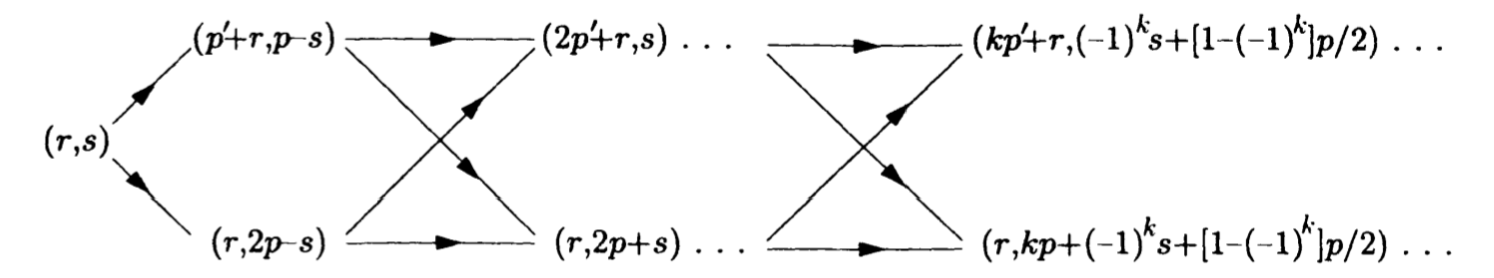
\includegraphics[width=\columnwidth]{/Users/sogenikegami/Documents/Research/Note/CFT/fig/fig1.png}
            \caption{}
            \label{fig1}
        \end{figure}
        結局既約表現は
        \begin{equation}\label{eq:irrmod1-10}
            M_{r,s} = V_{r,s} - (V_{p^\prime+r,p-s} \cup V_{r,2p-s}) + (V_{2p^\prime+r,s} \cup V_{r,2p+s}) - \cdots
        \end{equation}
        というふうに足し引きをして得られる。

        \subsubsection{指標}
        この無限に続く差し引きをシンプルに表現する方法として、既約表現$M_{r,s}$の指標がある。
        可約/既約を気にしない場合、Virasoro指標は
        \begin{equation}\label{eq:irrmod2-1}
            \chi_{(c,h)}(q) = \sum_{n=0}^\infty \dim(h+n)q^{h+n-c/24} = \frac{q^{h-c/24}}{\varphi(q)}
        \end{equation}
        と書けるのであった。式\eqref{eq:irrmod1-10}より、既約表現の指標は
        \begin{tcolorbox}
            \begin{align}\label{eq:irrmod2-2}
                \chi_{(r,s)}(q) = \frac{q^{-c/24}}{\varphi(q)} \left[ q^{h_{r,s}} + \sum_{k=1}^\infty (-1)^k  \left\{ q^{h_{r+kp^\prime,(-1)^ks+[1-(-1)^k]p/2}} \right. \right. \\
                \left.\left.  +q^{h_{r,kp+(-1)^ks+[1-(-1)^k]p/2}}  \right\}  \right] \notag
            \end{align}
        \end{tcolorbox}
        上式は関数
        \begin{equation}\label{eq:irrmod2-3}
            K_{r,s}^{(p,p^\prime)}(q) = \frac{q^{-1/24}}{\varphi(q)}\sum_{n\in \mathbb{Z}} q^{(2pp^\prime n+pr-p^\prime s)^2/4pp^\prime}
        \end{equation}
        によって
        \begin{tcolorbox}
            \begin{equation}\label{eq:irrmod2-4}
                \chi_{(r,s)}(q) = K_{r,s}^{(p,p^\prime)}(q) - K_{r,-s}^{(p,p^\prime)}(q)
            \end{equation}
        \end{tcolorbox}
        と表される。表\ref{fig2}に幾つかのミニマルモデルにおける指標の展開を示す。genericな(null状態がない)表現の指標は
        \begin{equation}\label{eq:irrmod2-5}
            \frac{1}{\prod_{n\geq 1}(1-q^n)} = 1 + q + 2q^2 + 3q^3 + 5q^4 + 7q^5+11q^6 + \cdots
        \end{equation}
        であることと表を見比べると、レベル$rs$で係数が落ちていることが確認できる。
        \begin{figure}[t]
            \centering
            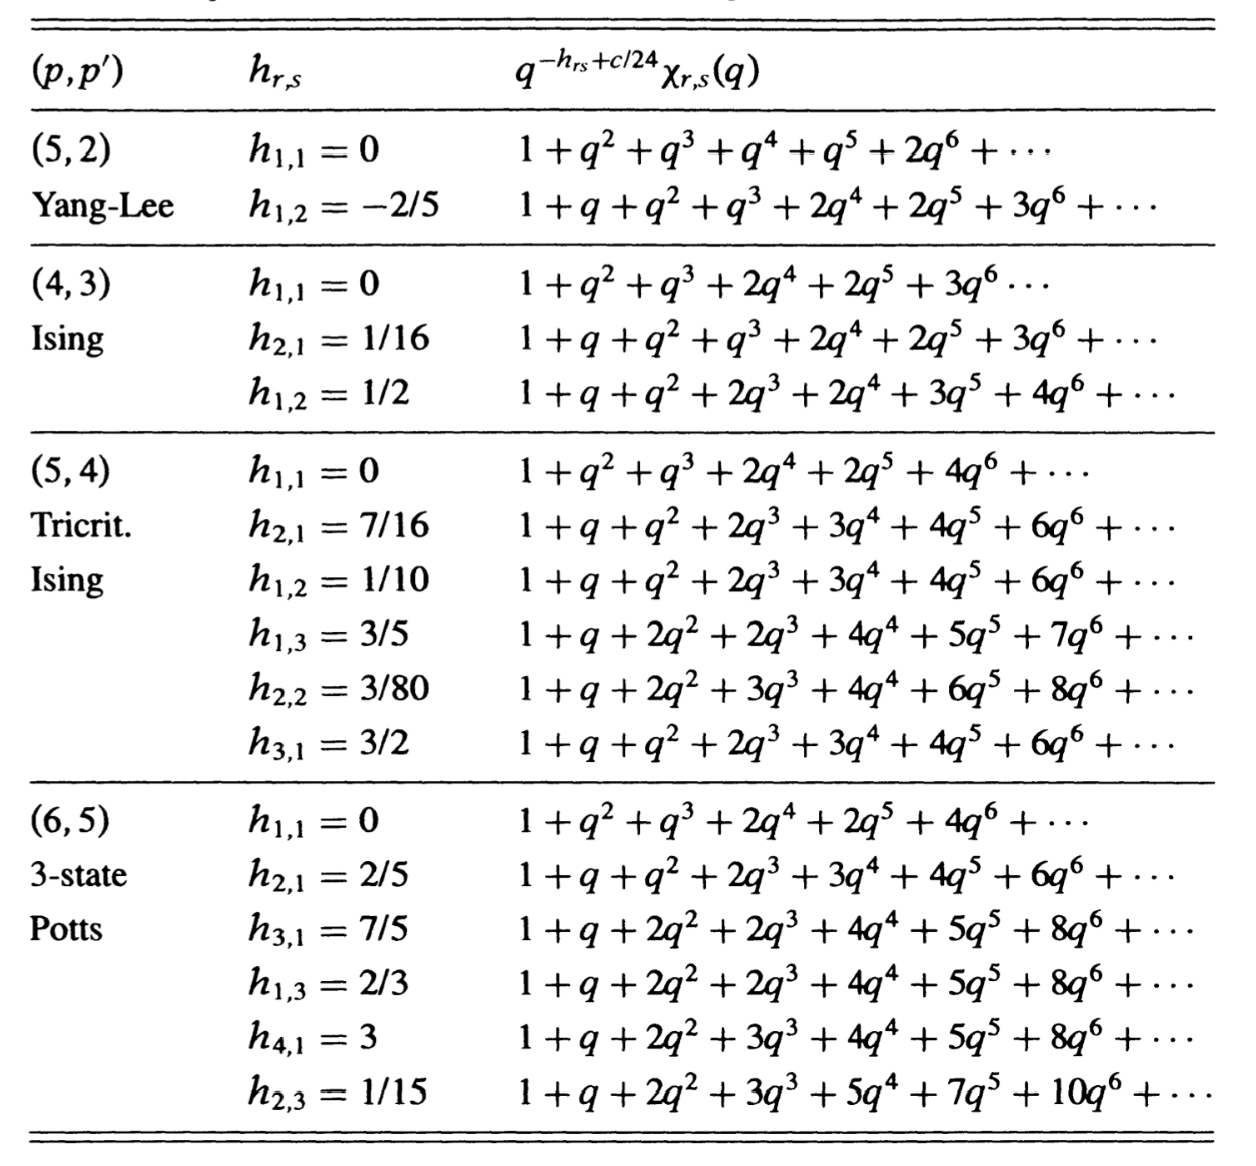
\includegraphics[width=0.8\columnwidth]{/Users/sogenikegami/Documents/Research/Note/CFT/fig/fig2.png}
            \caption{}
            \label{fig2}
        \end{figure}

    \subsection{explicit form of singular vectors}
    本節ではVerma加群$V_{r,s=1}$のレベル$r$におけるnull状態を具体的に構成する。
    戦略としては、各要素が$L_n$の線型結合で構成されるような行列を最高ウェイト状態に作用させ、その逆行列のようなものを考えるというものである。
    この行列はスピン$(r-1)/2$、すなわちSU(2)の$r$次元表現である。
    \begin{align}\label{eq:nullvec1}
        [J_0]_{i,j} &= \frac{1}{2}(r-2i+i)\delta_{i,j} \notag \\
        [J_-]_{i,j} &=\left\{\begin{array}{ll}
            \delta_{i,j+1} & (j=1,2,\cdots ,r-1) \\ 0 & (j=r)
        \end{array}\right. \\
        [J_+]_{i,j} &= \left\{\begin{array}{ll}
            i(r-1)\delta_{i+1,j} & (j=1,2,\cdots ,r-1) \\ 0 & (j=r)
        \end{array}\right. 
    \end{align}
    これらは交換関係
    \begin{equation}\label{eq:nullvec2}
        [J_+, J_-] = 2J_0, \quad [J_0,J_\pm] = \pm J_\pm
    \end{equation}
    を満たす。例えば$r=4$の場合、
    \begin{equation}\label{eq:nullvec3}
        J_0 = \frac{1}{2} \mqty(\dmat{3,1,-1,-3}), J_- = \begin{pmatrix}
            0 & & & \\ 1 & 0 & & \\ & 1 & 0 & \\ & & 1 & 0
        \end{pmatrix},
        J_+ = \begin{pmatrix}
            0 & 3 & & \\ & 0 & 4 & \\ & & 0 & 3 \\ & & & 0
        \end{pmatrix}
    \end{equation}
    である。これは通常の角運動量の昇降演算子とは異なる。しかし、昇降演算子はそれぞれ上三角・下三角なので冪零$J_+^r = J_-^r = 0$である。
    ここで、次の$r\times r$行列を考える。
    \begin{equation}\label{eq:nullvec4}
        D_{r,1}(t) = -J_- + \sum_{m=0}^{\infty} (-tJ_+)^m L_{-m-1}
    \end{equation}
    この演算子は各成分が状態となっているような$r$成分ベクトル$(f_1, \cdots, f_r)^T$に作用する。ここで、
    演算子$D$の行列式を形式的に定義しよう。まず、次の線型方程式
    \begin{equation}\label{eq:nullvec5}
        D_{r,1}(t) \begin{pmatrix}
            f_1 \\ f_2 \\ \vdots \\ f_r
        \end{pmatrix} = \begin{pmatrix}
            f_0 \\ 0 \\ \vdots \\ 0
        \end{pmatrix}
    \end{equation}
    を考える。この方程式から、$f_0, \cdots f_{r-1}$を$f_r$で表すことができる。
    例えば$D$の一番下の行は$[D]_{r,r-1}=-1, [D]_{r,r}=L_{-1}$でそのほかの要素は零であるから、
    \begin{equation}\label{eq:nullvec6}
        f_{r-1} = L_{-1}f_r
    \end{equation}
    となる。下から二行目はもう一つ非ゼロの要素が増えるので、$f_r, r_{r-1}, f_{r-2}$の間の関係式になるが、前の結果\eqref{eq:nullvec6}を使って
    $f_{r-2},f_{r}$だけの関係式にできる。このようにして、
    \begin{align}\label{eq:nullvec7}
        f_{r-2} &= [L_{-1}^2 - t(r-1)L_{-2}]f_r \\
        f_{r-3} &= [L_{-1}^3 - t(r-1)L_{-1}L_{-2} - 2t(r-2)L_{-2}L_{-1} + 2t^2(r-1)(r-2)L_{-3}]f_r \notag
    \end{align}
    と順次関係式を作れる。演算子の形式的な行列式を
    \begin{equation}\label{eq:nullvec8}
        f_0 = \Delta_{r,1}(t) f_r
    \end{equation}
    で表す。記号の扱いは乱暴であるが、この$\Delta$を
    \begin{tcolorbox}
        \begin{equation}\label{eq:nullvec9}
            \Delta_{r,1}(t) = \det \left[ -J_- + + \sum_{m=0}^{\infty} (-tJ_+)^m L_{-m-1} \right]
        \end{equation}
    \end{tcolorbox}
    と定義する。例えば、
    \begin{align}\label{eq:nullvec10}
        \Delta_{1,1}(t) &= L_{-1} \notag \\
        \Delta_{2,1}(t) &= L_{-1}^2 -t L_{-2}  \\
        \Delta_{3,1}(t) &= L_{-1}^3 -2t( L_{-1}L_{-2} + L_{-2}L_{-1}) + 4t^2L_{-3} \notag 
    \end{align}
    である。状態
    \begin{tcolorbox}
        \begin{equation}\label{eq:nullvec11}
            \ket{\chi_r} = \Delta_{r,1}(t)\ket{h_{r,1}(t)}
        \end{equation}
    \end{tcolorbox}
    はVerma加群$V_{r,1}$のレベル$r$のnull状態であることを示すことができる。これを示すには
    $L_0$の固有値$h+r$の固有状態$L_0\ket{\chi_r}=(h_{r,1}+r)\ket{\chi_r}$であり、$L_1,L_2$に対して消えることを言えば良い。
    
    (i)$L_0$について、その構成方法から、$f_r = \ket{h_{r,1}}$と最高ウェイト状態から始まり、$f_j$はレベル$r-j$に属することがわかる。
    言い換えると、式\eqref{eq:nullvec10}は昇降演算子の線型結合になっているが、どの項も同じレベルの状態を生成する。したがって
    $f_0 = \Delta_{r,1}\ket{h}$はレベル$r$に属し、$L_0\ket{\chi_r}=(h_{r,1}+r)\ket{\chi_r}$である。

    (ii)$L_1$を$f_j$に作用させると、$j=0,\cdots,r-1$に対して、
    \begin{equation}\label{eq:nullvec12}
        L_1f_j = \frac{j(r-j)}{2}[(2j+3-r)t-2]f_{j+1}
    \end{equation}
    となる。例えば$j=r-2$の場合、Virasoro代数を使って
    \begin{align}\label{eq:nullvec13}
        L_1f_{r-2} &= L_1 [L_{-1}^2 -t(r-1) L_{-2}]\ket{h_{r,1}} \notag \\
        &= L_{-1}L_1L_{-1} + 2L_{0}L_{-1} -3t(r-1)L_{-1}\ket{h_{r,1}} \notag \\
        &= 2L_{-1}L_0 + 2L_{-1}L_0 +2L_{-1} -3t(r-1) L_{-1}\ket{h_{r,1}} \notag \\
        &= (4h+2-3t(r-1))f_{r-1}
    \end{align}
    と計算できる。この式自体は帰納的に示すことができる。$j=0$のとき、まさに$L_1f_0 = 0$である。

    (iii)$L_2$に関しても、$f_i$に作用すると
    \begin{equation}\label{eq:nullvec14}
        L_2f_j = \frac{t}{4}j(r-j)(j+1)(r-j-1)\left[ (4j+6-r)t -7 \right]f_{j+2}
    \end{equation}
    となることが示せる。$j=0$が求める式である。いくつかコメントをし、本節を終える。
    
    (a)Verma系列$V_{1,s}$に関しても同様の関係式を導くことができる。この際には$r \rightleftarrows s$, $t \rightleftarrows 1/t$と変換をすれば良い。
    
    (b)$\Delta$に関して具体的に書き下すことができて、null状態は次のように書ける。
    \begin{tcolorbox}
        \begin{equation}\label{eq:nullvec15}
            \ket{\chi_r} = \sum_{\substack{p_i \geq 1 \\ p_1 + \cdots + p_k = r }} \frac{[(r-1)!]^2(-t)^{r-k}}{\prod_{i=1}^{k-1}(p_1 + \cdots + p_i)(r-p_1-\cdots -p_i)} L_{-p_1} \cdots L_{-p_k} \ket{h_{r,1}(t)}
        \end{equation}
    \end{tcolorbox}

    (c)$n>2$に関して$L_n$の$\mathbf{f}=(f_1,\cdots,f_r)^T$に対する作用をあらわに書くことができる。
    \begin{equation}\label{eq:nullvec16}
        L_n \mathbf{f} = \left[ \left( J_0 - \frac{3n+1}{2} \right) + \frac{3n+1}{4t} \right] (-tJ_+)^n \mathbf{f}
    \end{equation}
    本節ではVerma加群$V_{r,1}$のnull状態を導出したが、一般的な加群$V_{r,s}$について、null状態の閉じた表式は知られていない。
    しかし全く太刀打ちできないこともなく、Appendix8.Aで長大な導出が書かれている。

    \subsection{相関関数における微分方程式}
    ミニマルモデルにおけるプライマリー場はVirasoro代数の最高ウェイト状態にアタッチされるが、その表現が既約であることを要請するために
    全てのnull状態は0にセットされなければならない。これにより相関関数や演算子積展開に非自明な制約を与える。
    本節ではプライマリー場の相関関数がどのような制限を受けるのかを見ていく。
    その前に反正則部分に関するコメントをしておく。これまで正則部分に集中してみたいが、実際には反正則部分も付け加えてやらねばならない。
    ミニマルモデルにおいては正則・反正則部分に対応するVerma加群のペアを考えることになる。二つのVerma加群はどちらもKac tableにあり、
    それぞれが既約であるためにnull状態をゼロにセットする。これらは独立しており、正則部分と反正則部分で独立に制限がされる。複雑な部分は次章で扱う。

        \subsubsection{特異ベクトルによる微分方程式}
        場の理論における相関関数の計算の主要な道具なWard恒等式である。descendant場の相関関数をプライマリー場で表す際にも用いられたのであった。
        \begin{equation}\label{eq:vec-eq1-1}
            \expval{\phi_0^{-r_1,\cdots,-r_k}(z_0)\phi_1(z_1)\cdots} = \mathcal{L}_{-r_1}(z_0)\cdots \mathcal{L}_{-r_k}(z_0)\expval{\phi_0(z_0)\phi_1(z_1)\cdots}
        \end{equation}
        \begin{equation}\label{eq:vec-eq1-2}
            \mathcal{L}_{-r}(z) = \sum_{i \geq 1}\left\{ \frac{(r-1)h_i}{(z_i-z)^r} - \frac{1}{(z_i-z)^{r-1}}\partial_{z_i} \right\}
        \end{equation}
        左(=正則)Virasoro表現$\phi_0$は可約Verma加群$V(c,h_0)$であり、レベル$n_0$のnull状態は
        \begin{equation}\label{eq:vec-eq1-3}
            \ket{c,h_0+n_0} = \sum_{Y,|Y|=n_0}\alpha_Y L_{-Y}\ket{c,h_0}
        \end{equation}
        で与えられるとする。ここで$Y$は
        \begin{align}
            Y &= \left\{r_1,\cdots,r_k\right\} \quad \text{with} \quad 1\leq r_1 \leq \cdots \leq r_k \\
            |Y| &= r_1 + \cdots + r_k \\
            L_{-Y} &= L_{-r_1}L_{-r_2}\cdots L_{-r_k}
        \end{align}
        を省略している。特異ベクトルをゼロになることを要請すると、$\sum \alpha L_{-Y}\phi_0=0$であり、相関関数では
        \begin{equation}\label{eq:vec-eq1-4}
            \sum_{Y}\alpha_Y \mathcal{L}_{-Y}(z_0)\expval{\phi_0(z_0)\phi_1(z_1)\cdots} = 0
        \end{equation}
        となる。ここで特異ベクトル(の相関関数)が消える条件を微分方程式で表現するため、Ward恒等式\eqref{eq:vec-eq1-1}を用いた。
        前節に従って、$\Delta_0 = \sum_Y \alpha_Y L_{-Y}$をVerma加群$V(c,h_0)$の特異ベクトルを生成する演算子とする。
        相関関数の満たすべき微分方程式は相関関数$\expval{\phi_0(z_0)\phi_1(z_1)\cdots}$に微分演算子
        \begin{equation}\label{eq:vec-eq1-5}
            \gamma_0(z_i,\partial_{z_i}) = \Delta_0(L_{-r} \rightarrow \mathcal{L}_{-r}(z_0))
        \end{equation}
        を作用させると得られる。$L$はVirasoro代数の演算子で$\mathcal{L}$は\eqref{eq:vec-eq1-2}で定義される場に作用する演算子である。
        微分方程式\eqref{eq:vec-eq1-4}は大域共形変換による相関関数の不変性を用いるとさらにシンプルになる。
        少し大域共形不変性による相関関数の形を復習しておく。
        大域共形変換($SL(2,\mathbb{C}$))のWard恒等式による相関関数が満たす微分方程式は
        \begin{align}\label{eq:vec-eq1-6}
            \sum_{i=0,1,\cdots}\partial_{z_i}\expval{\phi_0(z_0)\phi_1(z_1)\cdots} &= 0 \notag \\
            \sum_{i=0,1,\cdots}(z_i\partial_{z_i}+h_i)\expval{\phi_0(z_0)\phi_1(z_1)\cdots} &= 0 \\
            \sum_{i=0,1,\cdots}(z_i^2\partial_{z_i}+2z_ih_i)\expval{\phi_0(z_0)\phi_1(z_1)\cdots} &= 0 \notag
        \end{align}
        であった。これは解くことができて、
        \begin{equation}\label{eq:vec-eq1-7}
            \expval{\phi_0(z_0)\phi_1(z_1)\cdots}  = \left\{ \prod_{i<j} (z_i-z_j)^{\mu_{ij}} \right\}G({z_{ij}^{kl}})
        \end{equation}
        となるのであった。ここで$\mu_{ij}$は
        \begin{equation}\label{eq:vec-eq1-8}
            \sum_{j\neq i}\mu_{ij} = 2h_i
        \end{equation}
        の任意の解で、$G$はanharmonic ratio
        \begin{equation}\label{eq:vec-eq1-9}
            z_{ij}^{kl} = \frac{(z_i-z_j)(z_k-z_l)}{(z_i-z_l)(z_k-z_j)}
        \end{equation}
        の任意の関数である。よって式\eqref{eq:vec-eq1-4}の相関関数は大域共形変換の不変性によって、\eqref{eq:vec-eq1-7}に微分演算子が作用したものとなる。

        式\eqref{eq:vec-eq1-4}の具体例を二つ見る。
        一つ目はシンプルなケースで、Verma加群$V(c,h)=V_{r=2,s=1}$を考える。最初のnull状態はレベル$rs=2$に現れ、$\Delta_0$は
        \begin{equation}\label{eq:vec-eq1-10}
            \Delta_0 \equiv \Delta_{2,1}(t) = L_{-1}^2 - tL_{-2}
        \end{equation}
        である。従って相関関数の満たす微分方程式は
        \begin{equation}\label{eq:vec-eq1-11}
            \left\{ \partial_z^2 -t\sum_{i=1,2,\cdots}\left[ \frac{h_i}{(z_i-z)^2} - \frac{1}{z_i-z}\partial_{z_i} \right] \right\} \expval{\phi_{(2,1)}(z)\phi_1(z_1)\cdots} = 0
        \end{equation}
        となる。これは2階の偏微分方程式であり、二つの線型独立な解がある。さらに高いレベルのnull状態に対する制限もまた考えることができる。

        もう一つの例は$V(c,h)=V_{r,1}$の場合で、レベル$rs=r$で初めてnull状態が現れる。前節から、微分作用素の具体的な表式を書くことができて、
        \begin{align}
            \gamma_{r,1}(z_i,\partial_{z_i}) &\equiv \det D_{r,1}(z_i,\partial_{z_i}) \\
            &= \det \left[ -J_- + \partial_{z_0} + \sum_{m\geq1}(-tJ_+)^m \sum_{j\geq1}\left( \frac{mh_i}{(z_i-z)^{m+1}} - \frac{1}{(z_i-z)^m} \partial_{z_i} \right) \right]
        \end{align}
        であり、$r$階の偏微分方程式は
        \begin{equation}\label{eq:vec-eq1-12}
            \gamma_{r,1}(z_i,\partial_{z_i})\expval{\phi_{r,1}(z_0)\phi_1(z_1)\cdots} = 0
        \end{equation}
        となる。前節でdeterminantを形式的に定義したが、今回はそれに基づいてベクトルと行列作用素の方程式に戻すことができる。
        \begin{equation}\label{eq:vec-eq1-13}
            D_{r,1}(z_i,\partial_{z_i})\mathbf{f} = 0
        \end{equation}
        ここで$f$ベクトルの最後の要素が
        \begin{equation}\label{eq:vec-eq1-14}
            f_r = \expval{\phi_{0}(z_0)\phi_1(z_1)\cdots}
        \end{equation}となっている。

        \subsubsection{ミニマルモデルにおける2点関数の微分方程式}
        これまでにみたように、大域共形変換の普遍性から2点、3点相関関数は係数を除いて完全に決定されるのであった。
        本節ではnull状態がゼロであるという条件から、係数に関する条件である一種のsum ruleを導くことができる。
        スタート地点は2点関数の表式
        \begin{equation}\label{eq:vec-eq2-1}
            \expval{\phi_{h_0}(z)\phi_{h_1}(0)} = \delta_{h_0,h_1}z^{-2h_0}
        \end{equation}
        これは微分方程式\eqref{eq:vec-eq1-4}を満たすことをチェックできる。
        \begin{equation}\label{eq:vec-eq2-2}
            \Delta_0 \left( L_{-r} \rightarrow \frac{(r-1)h_0}{(w-z)^r} - \frac{1}{(w-z)^{r-1}}\partial_w \right) \expval{\phi_0(z)\phi_0(w)} = 0
        \end{equation}
        並進対称性から2点関数は$x=z-w$の関数になっており、
        \begin{equation}\label{eq:vec-eq2-3}
            \Delta_0 \left( L_{-r} \rightarrow \frac{(-1)^r}{x^r} [(r-1)h_0 - x\partial_x] \right) \expval{\phi_0(x)\phi_0(0)} = 0
        \end{equation}
        非減少な整数列$Y$に対し、相関関数の$\mathcal{L}_{-Y}$の相関関数への作用は
        \begin{equation}\label{eq:vec-eq2-4}
            \expval{\phi_0(x)\phi_0(0)} = x^{-2h_0}\bar{x}^{-2\bar{h}_0},
        \end{equation}
        \begin{align}\label{eq:vec-eq2-5}
            \frac{(-1)^{|Y|}}{x^{|Y|}}\prod_{i=1}^{k}&[(r_i-1)h_0 -x\partial_x]\expval{\phi_0(x)\phi_0(0)} \notag \\
            &=\frac{(-1)^{|Y|}}{x^{|Y|}}\prod_{i=1}^{k}[(r_i+1)h_0 + r_{i+1}+\cdots +r_k] = 0
        \end{align}
        式\eqref{eq:vec-eq2-2}が満たされる必要十分条件は$\Delta_0=\sum_Y \alpha_Y L_{-Y}$の係数に関する次のsum ruleが満たされることである。
        \begin{equation}\label{eq:vec-eq2-6}
            \sum_{\substack{i\leq r_1\leq\cdots \leq r_k \\ \sum r_i=n_0}}\alpha_{r_1,r_2\cdots,r_k} \prod_{i=1}^k [(r_i+1)h_0 + r_{i+1} + \cdots + r_k] = 0
        \end{equation}
        実はこれはnull状態が満たすべき性質の一つ
        \begin{equation}\label{eq:vec-eq2-7}
            L_1^{n_0} \sum_{Y,|Y|=n_0}\alpha_Y L_{-Y}\ket{c,h_0} = 0
        \end{equation}
        から得られる結果となっている。まず、任意の整数列$r_1,\cdots,r_k, r_1 + \cdots + r_k=n_0$に対して
        \begin{equation}\label{eq:vec-eq2-8}
            L_1^{n_0}L_{-r_1}\cdots L_{-r_k}\ket{c,h_0} = P(r_1,\cdots,r_k;h_0)\ket{c,h_0}
        \end{equation}
        となっていることは明らかだろう。つまり最高ウェイト状態から出発して、$r_1 + \cdots + r_k=n_0$段降りた後$n_0$だけ戻ってきたら
        係数つきで最高ウェイト状態に戻っている。ここで$P$は$h_0,r$に関する多項式である。$P$に関して少し考察を進めてみる。
        $L_1^{n_0}=L_1^{n_0-1}L_1$とかくと、$P$に関する関係式を導くことができる。一つの$L_1$を交換関係を使って右に出していく。その過程で
        $k$個のnonzeroな項が出てくる。これにより、
        \begin{equation}\label{eq:vec-eq2-9}
            P(r_1,\cdots,r_k;h_0) = \sum_{i=1}^k (r_i+1)P(r_1,\cdots,r_{i-1},r_i-1,r_{i+1},\cdots,r_k;h_0)
        \end{equation}
        これを用いて$P$の中の引数を一つ減らすことができる。では$r_i=0$となる場合にはどうなるであろうか。これは
        定義式\eqref{eq:vec-eq2-8}で$r_i=0$、つまり$L_0$を間に挿入していることに対応しているので、そこまでで降りたレベルの数$+h$が出てくる。ゆえに
        \begin{align}\label{eq:vec-eq2-10}
            P(r_1,\cdots,r_{i-1},&0,r_{i+1},\cdots,r_k;h_0) = \notag \\
            &[h_0 + r_{i+1} + \cdots r_k]P(r_1,\cdots,r_{i-1},r_{i+1},\cdots,r_k;h_0)
        \end{align}
        となる。$k=1,n_0=r_1=r$とした時の結果
        \begin{equation}\label{eq:vec-eq2-11}
            L_1^rL_{-1}^r\ket{c,h_0} = P(r;h_0)\ket{c,h_0} = (r+1)!h_0\ket{c,h_0}
        \end{equation}
        から$P$を完全に決定することができて、
        \begin{equation}\label{eq:vec-eq2-12}
            P(r_1,\cdots,r_k;h_0) = (n_0!)\prod_{i=1}^k [(r_i+1)h_0 + r_{i+1} + \cdots + r_k]
        \end{equation}
        となる。式\eqref{eq:vec-eq2-7}からこれは$n_0!$を別にしてsum ruleを再現している。
        2点相関関数の係数が決定されたら、全ての相関関数の比例係数がfixされる。

        \subsubsection{ミニマルモデルにおける4点関数の微分方程式}
        本節ではミニマルモデル$\phi_{2,1}$における4点相関関数が満たす微分方程式を見ていく。結果として、
        超幾何関数が満たす方程式である超幾何方程式を得る。

        4点相関関数は2,3点関数とは異なり、大域共形不変性ではangarmonic ratioに関する任意の関数というところまでしか決定されないのであった。
        具体的には
        \begin{equation}\label{eq:vec-eq3-1}
            \expval{\phi_0(z_0)\phi_1(z_1)\phi_2(z_2)\phi_3(z_3)} = \prod_{0\leq i<j \leq3} (z_i-z_j)^{\mu_{ij}}G(z)
        \end{equation}
        \begin{equation}\label{eq:vec-eq3-2}
            \mu_{ij} = \frac{1}{3}\left( \sum_{k=1}^4 h_k \right) - h_i - h_j
        \end{equation}
        \begin{equation}\label{eq:vec-eq3-3}
            z = \frac{(z_0-z_1)(z_2-z_3)}{(z_0-z_3)(z_2-z_1)}
        \end{equation}
        であった。ここから微分方程式\eqref{eq:vec-eq1-4}の帰結を見ていく。最終的に$G$の常微分方程式に帰着する。これを(比較的)簡単な場合である$V_{2,1}$のレベル2
        についてみていく。この簡単なミニマルモデルの場合の相関関数が満たす微分方程式は
        式\eqref{eq:vec-eq1-11}であった。これに\eqref{eq:vec-eq3-1}を代入すれば良い。
        $\partial_{z_i}$の\eqref{eq:vec-eq3-1}への作用は、
        \begin{align}\label{eq:vec-eq3-4}
            \partial_{z_0} &= \frac{\mu_{01}}{z_0-z_1} + \frac{\mu_{02}}{z_0-z_2} + \frac{\mu_{03}}{z_0-z_3} + \partial_{z_0}(z)\partial_z, \quad \partial_{z_0}(z) = \frac{(z_3-z_1)(z_2-z_3)}{(z_2-z_1)(z_0-z_3)^2} \notag \\
            \partial_{z_1} &= -\frac{\mu_{01}}{z_0-z_1} + \frac{\mu_{12}}{z_1-z_2} + \frac{\mu_{13}}{z_1-z_3} + \partial_{z_1}(z)\partial_z, \quad \partial_{z_1}(z) = \frac{(z_0-z_2)(z_2-z_3)}{(z_0-z_3)(z_2-z_1)^2}  \\
            \partial_{z_2} &= -\frac{\mu_{02}}{z_0-z_2} - \frac{\mu_{12}}{z_1-z_2} + \frac{\mu_{23}}{z_2-z_3} + \partial_{z_2}(z)\partial_z, \quad \partial_{z_2}(z) = -\frac{(z_1-z_3)(z_0-z_1)}{(z_0-z_3)(z_2-z_1)^2} \notag \\
            \partial_{z_3} &= -\frac{\mu_{03}}{z_0-z_3} - \frac{\mu_{13}}{z_1-z_3} - \frac{\mu_{23}}{z_2-z_3} + \partial_{z_3}(z)\partial_z, \quad \partial_{z_3}(z) = \frac{(z_2-z_0)(z_0-z_1)}{(z_2-z_1)(z_0-z_3)^2} \notag 
        \end{align}
        である。また$\partial_{z_0}^2$の作用は
        \begin{align}\label{eq:vec-eq3-5}
            \partial_{z_0}^2 &= \frac{\mu_{01}(\mu_{01}-1)}{(z_0-z_1)^2} + \frac{\mu_{02}(\mu_{02}-1)}{(z_0-z_2)^2} + \frac{\mu_{03}(\mu_{03}-1)}{(z_0-z_3)^2} \notag \\
            & \ + 2\left[ \frac{\mu_{01}}{z_0-z_1} + \frac{\mu_{02}}{z_0-z_2} + \frac{\mu_{03}}{z_0-z_3} \right] \partial_{z_0}(z)\partial_z \notag \\
            & \ + \partial_{z_0}^2(z)\partial_z + (\partial_{z_0}(z))^2\partial_z^2
        \end{align}
        これらを代入すると、実は$G$の前の$(z_i-z_j)$を微分方程式の前に括り出すことができる。
        そうした後、$z_1\rightarrow 0, z_2\rightarrow 1, z_3\rightarrow \infty, z_0\rightarrow z$とすることで
        $G(z)$に関する常微分方程式を得ることができる。各点を上述の点に飛ばすことで、
        \begin{align}\label{eq:vec-eq3-6}
            \partial_{z_0} &= \frac{\mu_{01}}{z} + \frac{\mu_{02}}{z-1} + \partial_z \notag \\
            \partial_{z_1} &= -\frac{\mu_{01}}{z} - \mu_{12} + (z-1)\partial_z \notag \\
            \partial_{z_2} &= -\frac{\mu_{02}}{z-1} + \mu_{12} + z\partial_z  \\
            \partial_{z_3} &= 0 \notag \\
            \partial_{z_0}^2 &= \frac{\mu_{01}(\mu_{01}-1)}{z^2} + \frac{\mu_{02}(\mu_{02}-1)}{(z-1)^2}  \notag \\
            &+ 2\left[ \frac{\mu_{01}}{z} + \frac{\mu_{02}}{z-1} \right]\partial_z + \partial_z^2 \notag 
        \end{align}
        となり、結局$G$の微分方程式は
        \begin{align}\label{eq:vec-eq3-7}
            \left\{ \frac{1}{t}\partial_z^2 + [2\frac{\mu_{01}}{t(z-1)} + 2\frac{\mu_{02}}{t(z-1)} + \frac{2z-1}{z(z-1)}]\partial_z + \frac{\mu_{01}(\mu_{01}-1)}{tz^2} \right. \notag \\
            \left. + \frac{\mu_{02}(\mu_{02}-1)}{t(z-1)^2} + \frac{\mu_{01}-h_1}{z^2} + \frac{\mu_{02}-h_2}{(z-1)^2}-  \frac{\mu_{12}}{z(z-1)}  \right\}G(z) = 0
        \end{align}
        一見長い方程式だが、関数
        \begin{equation}\label{eq:vec-eq3-8}
            H(z) = z^{\mu_{01}}(1-z)^{\mu_{02}}G(z)
        \end{equation}
        を導入すると、
        \begin{equation}\label{eq:vec-eq3-9}
            \left\{ \frac{1}{t}\partial_z^2 + \frac{2z-1}{z(z-1)}\partial_z - \frac{h_1}{z^2} - \frac{h_2}{(z-1)^2} + \frac{h_0 + h_1 + h_2 + h_3}{z(z-1)} \right\}H(z) = 0
        \end{equation}
        これは超幾何方程式に変形することができて、超幾何級数が解となる。(演習問題)

        一般的に、$\phi_{r,s}$があるような相関関数は$rs$階の微分方程式を満たさねばならない。それに対応して$rs$個の
        線型独立な解が存在し、それらは相関関数の共形ブロックと呼ばれる。フルな相関関数は正則部分と反正則部分の半双線形形式である。
        ($f$が半双線形形式であるとは$f:V\times V\rightarrow \mathbb{C}, x,y,z,w\in V, a,b\in \mathbb{C}$に対して$f(x+y,z+w)=f(x,w)+f(x,w)+f(y,z)+f(y,w)$かつ$f(ax,by)=a^*bf(x,y)$であるような$f$のこと。)
        どの正則ブロックとどの反正則ブロックが積を組むかは対称性などによって決められる。これは次章で扱う。

        $rs$は相関関数が満たす微分方程式のうち、最低次(階)でない可能性がある。対称性$\phi_{p^\prime-r,p-s}\equiv \phi_{r,s}$は相関関数がまた
        $(p^\prime-r)(p-s)$階の微分方程式も満たすことを示している。この問題を少しだけ簡単にすることができる。まず$rs=N,(p^\prime-r)(p-s)=N+a$とおく。
        最初の方程式を$a$回微分することで、二つ目の方程式の最高次を消去することができる。このようにして二つ目の方程式の次数を減らしていくと、あるステップで
        二つの微分方程式が独立でなくなる。その時点で最低次がわかる。

        上記のように複数の高次微分方程式を解くことでミニマルモデルにおける相関関数は完全に決定される。しかし、次章で扱うCoulomb gasのformalismはより
        効率的な相関関数の計算方法を与える。この方法はfree bosonの相関関数の線積分によって、微分方程式を自動的に満たすような解を導くことができる。

    \subsection{Fusion rules}
    ミニマルモデルにおけるプライマリー場はKac tableの最高ウェイト状態に対応しているのであった。本節ではこれらの間のfusion rule、つまり二つの場の
    短距離積においてどのプライマリー場・descendant場が出てくるかをみる。前節で見た相関関数が満たす微分方程式はfusion ruleをsystematicに調べる方法を与える。
    また$(p,p^\prime)$ミニマルモデルは二つの基本的な場$\phi_{(2,1)},\phi_{(1,2)}$のfusionから生成されることを見る。

        \subsubsection{微分方程式によるFusion rule}
        ここでは前節で導出した相関関数の微分方程式からfusion ruleを導出する。その前にfusion ruleを振り返っておく。
        レベル2の特異ベクトルを持つ時、その特異ベクトルがゼロになるという条件から、3点相関関数の係数$g(h,h_1,h_2)$の三つの共形次元が完全に独立ではなくなり、
        $h$が制限されるのであった。この結果、$\phi_{2,1}$と$\phi_{(\alpha)}$のプライマリー場における演算子積展開を考えるときに展開時に現れるのが許される場が制限されることをfusion ruleというのであった。
        また複数の同値な場のfusion ruleを考えることによりさらに制限を強くできて、これをtruncationと呼んだ。逆にいうと、fusion ruleは一般の演算子積展開
        \begin{align}\label{eq:fusion1-1}
            \phi_0(z)\phi_1(w) &= (z-w)^{h-h_1-h_0}\sum_{h}g(h_0,h_1,h) \notag \\
            &\times \sum_Y (z-w)|Y| \beta_Y(h_0,h_1,h)L_{-Y}\phi(w)
        \end{align}
        の中に現れる$g(h,h_1,h_2)$のなかの$h$を$h_1,h_2$で表すことに対応する。
        一方で、上記の演算子積展開を前節で得た相関関数の微分方程式\eqref{eq:vec-eq1-4}に代入すると、係数$g,h$に関する制限を得ることができて、
        \begin{align}\label{eq:fusion1-2}
            \sum_h g(h_0,h_1,h) &\sum_Y \beta_Y(h_0,h_1,h)\gamma_0(z_i,\partial_{z_i}) \notag \\
            &\times (z_0-z_1)^{h-h_1-h_0+|Y|}\expval{[L_{-Y}\phi](z_1)\phi_2(z_2)\cdots} = 0
        \end{align}
        となる。$z_0 \rightarrow z_1$による極限での主要項は$|Y|=0, \beta=1, h$最大で、$z_0,z_1$に関する微分が高階であるような項になる。(?)
        このleading termが$h,h_0,h_1$に非自明な関係を与え、fusion ruleを与える。

        例としてVerma加群$V_{2,1}$を考える。4点相関関数において、式\eqref{eq:fusion1-2}は三つの項からなる。
        $\partial_{z_0}^2, (z_0-z_1)^{-2}, (z_0-z_1)^{-1}\partial_{z_0}$である。
        ここから、
        \begin{equation}\label{eq:fusion1-3}
            \frac{1}{t}(h-h_0-h_1)(h-1-h_0-h_1)+(h-h_0-h_1)-h_1 = 0
        \end{equation}
        という制限が得られる。$r=2,s=1$なので、
        \begin{equation}\label{eq:fusion1-4}
            h_0 = h_{2,1}(t) = \frac{3}{4}t-\frac{1}{2}
        \end{equation}
        であり、$h_1$はミニマルKac tableの中の$h_1 = h_{r,s}(t),t=p_p^\prime$であるとする。
        すると\eqref{eq:fusion1-3}は変形できて、
        \begin{align}\label{eq:fusion1-5}
            \left( h-h_0-h_1-\frac{1-t}{2} \right)^2 &= \left( \frac{1-t}{2} \right)^2 + th_1 \notag \\
            &= \left( \frac{1-t}{2} \right)^2 + \frac{t^2}{4}(r^2-1) + \frac{1}{4}(s^2-1) - \frac{t}{2}(rs-1) \notag \\
            &= \frac{t^2r^2+s^2-2trs}{4} \notag \\
            &= \left( \frac{tr-s}{2} \right)^2
        \end{align}
        となる。よって
        \begin{equation}\label{eq:fusion1-6}
            h = h_0 + h_1 + \frac{1-t}{2} \pm \frac{tr-s}{2} = h_{r+\epsilon,s}(t) \quad \epsilon = \pm1
        \end{equation}
        つまり、特異ベクトルがゼロであるという条件を4点相関関数の微分方程式に落とし込み、そこに演算子積展開に使うと三つの共形次元の間の関係式が得られたのである。
        さらに言えば、三つのうち二つの場をミニマルモデルのプライマリー場とすると、三つ目の場もKac公式にのるミニマルモデルとなった。
        ここから、次のfusion ruleがわかる。
        \begin{equation}\label{eq:fusion1-7}
            \phi_{(2,1)}\times \phi_{(r,s)} = \phi_{(r-1,s)} + \phi_{(r+1,s)}
        \end{equation}
        厳密に言えば、これは微分方程式の主要項のみを見て得られた結果であり、さらに詳しく調べると二つのどちらかが削れるなどがあるかもしれない。
        しかし、
        \begin{equation}\label{eq:fusion1-8}
            h_{r+1,s}(p,p^\prime) - h_{r-1,s}(p,p^\prime) = r\frac{p}{p^\prime}-s
        \end{equation}
        であり、これはKac tableの中で整数を取らない。したがって、descendant場の寄与などから制限は生まれず、
        どちらのプライマリー場も残ることになる。

        より一般的に$V(c,h)=V_{r,1}$としよう。こちらはappendixの長い内容を必要とするため簡潔に見ていくことにする。
        ただしやることは先ほどと同様で、相関関数の微分方程式\eqref{eq:vec-eq1-5}から始まり、演算子積展開\eqref{eq:fusion1-1}
        を代入し$z_0 \rightarrow z_1$による主要項をみる。これが消える必要があることから共形次元の間の制限が得られ、
        fusion ruleを得ることができる。
        主要項は$\gamma_{r,1}$の中でも$(z_0-z_1),\partial_{z_0}, \partial_{z_1}$
        を抜き出すことと等価であるので、$\gamma_{r,1}$の中の主要項を抜き出した$\tilde{\gamma}_{r,1}$を
        \begin{align}\label{eq:fusion1-9}
            L_{-r} &\rightarrow \frac{(r-1)h_1}{(z_1-z_0)^r} - \frac{1}{(z_1-z_0)^{r-1}}\partial_{z_1} \\
            L_{-1} &\rightarrow \partial_z \notag
        \end{align}
        $\Delta_{r,1}(t)$に代入したもので定義する。演算子$\tilde{\gamma}_{r,1}$は演算子積展開のleading term$z^{h-h_0-h_1}$
        に作用する。すると、間を割愛するが結果として
        \begin{align}\label{eq:fusion1-10}
            (\theta_{r,1})^2 &= \prod_{m=1}^r \left\{ [h_0+h_1-h+(r-m)(1-tm)]  \right. \notag \\
            & \left. \times[h_0+h_1-h+(m+1)(1-t(r+1-m))] - 4h_1t(\frac{r+1}{2}-m)^2 \right\}
        \end{align}
        として、fusionが許されるのは
        \begin{equation}\label{eq:fusion1-11}
            \theta_{r,1}^2 = 0
        \end{equation}
        が必要十分条件となる。ここに$h_0 = h_{r,1}(t), h_1 = h_{k,l}(t)$を代入すると、結局$k\geq r, k+r\leq p^\prime$で許されるfusionは
        \begin{equation}\label{eq:fusion1-12}
            \phi_{(r,1)} \times \phi_{(k,l)} = \sum_{\substack{m=k-r+1 \\ m-k+r-1 \text{even} }}^{k+r-1} \phi_{(m,l)}
        \end{equation}
        もし$k$が$r$か$p^\prime -r$よりおおきい場合はもう少し複雑な結果となる。

        \subsubsection{Fusion Algebra}
        fusion number $\mathcal{N}_{ij}^k \in \left\{ 0, 1\right\}$を定義する。定義は
        \begin{equation}\label{eq:fusion2-1}
            \mathcal{N}_{ij}^k = \left\{ \begin{array}{ll}
                0 & g(h_i,h_j,h_k)=0 \\ 1 & \text{otherwise}
            \end{array} \right.
        \end{equation}
        である。インデックス$i,j,k$はKac tableの中のラベリングでも良いが、さらに一般的なプライマリー場のラベルと思って問題ない。
        反正則部分も考えるとfusion numberは$\mathcal{N}_{\text{left}}\times \mathcal{N}_{\text{right}}$となる。
        fusion numberと生成子$\phi_j, j=1,\cdots,r, \phi_1 = I$、それに積によりmultiplication rule
        \begin{tcolorbox}
            \begin{equation}\label{eq:fusion2-2}
                \phi_i \times \phi_j = \sum_k \mathcal{N}_{ij}^k \phi_k
            \end{equation}
        \end{tcolorbox}
        によりfusion algebraと呼ばれる。特に、identity$\phi_1$の積は
        \begin{equation}\label{eq:fusion2-3}
            \mathcal{N}_{i1}^k = \delta_{i,k}
        \end{equation}
        となり、積の可換性はシンプルに
        \begin{equation}\label{eq:fusion2-4}
            \mathcal{N}_{ij}^k = \mathcal{N}_{ji}^k
        \end{equation}
        となる。プライマリー場の演算子積展開の結合性もfusion algebraの結合性により表される。
        \begin{align}\label{eq:fusion2-5}
            \phi_i \times (\phi_j \times \phi_k) &= \phi_i \times \sum_{l}\mathcal{N}_{jk}^l \phi_l \\
            &= \sum_{l,m}\mathcal{N}_{jk}^l \mathcal{N}_{il}^m \phi_m
        \end{align}
        と
        \begin{align}\label{eq:fusion2-6}
            (\phi_i \times \phi_j) \times \phi_k &= \sum_l \mathcal{N}_{ij}^l \phi_l \times \phi_k \\
            &= \sum_{l,m}\mathcal{N}_{ij}^l \mathcal{N}_{lk}^m \phi_m
        \end{align}
        から、
        \begin{tcolorbox}
            \begin{equation}\label{eq:fusion2-7}
                \sum_{l} \mathcal{N}_{kj}^l \mathcal{N}_{il}^m = \sum_{l}\mathcal{N}_{ij}^l \mathcal{N}_{lk}^m
            \end{equation}
        \end{tcolorbox}
        を得る。Lie代数において構造定数から随伴表現を構成するように、$r\times r$行列を$N_i$で定義し、その要素を
        \begin{equation}\label{eq:fusion2-8}
            (N_i)_{j,k} = \mathcal{N}_{ij}^k
        \end{equation}
        で定義すると、結合性の条件\eqref{eq:fusion2-7}は通常の行列積で言い換えられて、
        \begin{equation}\label{eq:fusion2-9}
            N_i N_k = N_k N_i
        \end{equation}
        となる。また\eqref{eq:fusion2-7}は別のようにも書き換えられて、
        \begin{equation}\label{eq:fusion2-10}
            N_iN_k = \sum_{l} \mathcal{N}_{ik}^l N_l
        \end{equation}
        とも表される。したがって$\mathcal{N}$はfusion代数の表現をなす。

        \subsubsection{ミニマルモデルにおけるFusion Rules}
        ミニマルモデル$\mathcal{M}(p,p^\prime)$におけるfusion ruleに戻ろう。
        混乱を避けるために、前節で扱ったfusion numberのインデックスを$(r,s)$でしっかり書くことにする。例えば
        \begin{equation}\label{eq:fusion3-1}
            \mathcal{N}_{(1,1)(r,s)}^{(m,n)} = \delta_{r,m}\delta_{s,n}
        \end{equation}
        であり、
        \begin{align}\label{eq:fusion3-2}
            \mathcal{N}_{(2,1)(r,s)}^{(m,n)} &= \delta_{s,n} (\delta_{m,r+1} + \delta_{m,r-1}) \notag \\
            \mathcal{N}_{(1,2)(r,s)}^{(m,n)} &= \delta_{m,r} (\delta_{n,s+1} + \delta_{n,s-1})
        \end{align}
        となる。特に$\phi_{2,1},\phi_{1,2}$はそれぞれ$r,s$に対する昇降演算子のような役割を果たしている。
        本節の主要な結果は、$\phi_{2,1},\phi_{1,2}$のfusionが他のすべてのプライマリー場(とその共形族)を多項式的に生成するという事実である(Fig.~\ref{fig3})。

        \begin{figure}[t]
            \centering
            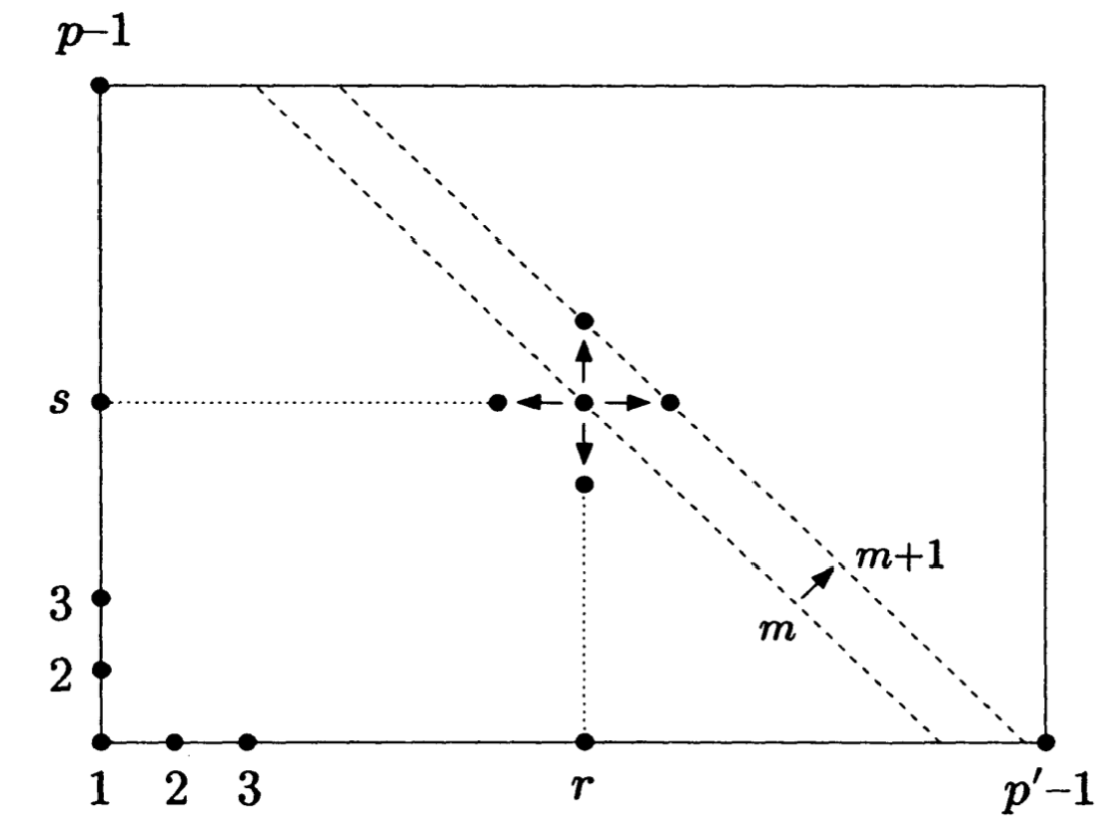
\includegraphics[width=0.7\columnwidth]{/Users/sogenikegami/Documents/Research/Note/CFT/fig/fig3.png}
            \caption{}
            \label{fig3}
        \end{figure}

        多項式的にというのは、随伴表現を作るように定義した行列$N_{(r,s)}$が$N_{(2,1)},N_{(1,2)}$の多項式で生成されるという意味である。
        もう少し具体的に、行列形式では$X=N_{(2,1)},Y=N_{(1,2)}$とすると、式\eqref{eq:fusion3-2}は
        \begin{equation}\label{eq:fusion3-3}
            N_{(r+1,1)} = XN_{(r,1)} - N_{(r-1,1)}
        \end{equation}
        となる。初期条件は
        \begin{equation}\label{eq:fusion3-4}
            N_{(1,1)} = I, \quad \text{and} \quad N_{(2,1)} = X
        \end{equation}
        である。実はこれは第二種チェビシェフ多項式が満たす漸化式になっている。第二種チェビシェフ多項式は
        \begin{equation}\label{eq:fusion3-5}
            U_m(2\cos \theta) = \frac{\sin(m+1)\theta}{\sin \theta}
        \end{equation}
        で定義され、その漸化式は
        \begin{equation}\label{eq:fusion3-6}
            U_m(x) = xU_{m-1}(x) - U_{m-2}(x)
        \end{equation}
        \begin{equation}
            U_0(x) = 1, \quad \text{and} \quad U_1 = x
        \end{equation}
        であるので、まさしく\eqref{eq:fusion3-3}である。したがって、直ちに行列$N$がわかって
        \begin{equation}\label{eq:fusion3-7}
            N_{(r,1)} = U_{r-1}(X), \quad N_{(1,s)} = U_{s-1}(Y)
        \end{equation}
        となる。Kac tableは$r=p^\prime, s=p$の長方形の内側であった。したがって、行列のKac tableにおける境界条件は
        \begin{equation}\label{eq:fusion3-8}
            N_{(r,0)} = N_{(r,p)} = N_{(0,s)} = N_{(p^\prime,s)} = 0
        \end{equation}
        である。これはチェビシェフ多項式の二つの制限を意味する。
        \begin{tcolorbox}
            \begin{equation}\label{eq:fusion3-9}
                U_{p^\prime -1}(X) = 0, \quad U_{p-1}(Y) = 0
            \end{equation}
        \end{tcolorbox}
        今Kac tableの$r=1, s=1$の一次元方向にのみ行列を帰納的に構成したが、一般の点についても構成しよう。
        こちらも簡単で、結果は
        \begin{equation}\label{eq:fusion3-10}
            N_{(r,s)} = U_{r-1}(X)U_{s-1}(Y)
        \end{equation}
        である。こちらも帰納的に示すことができる。したがって、前述のようにミニマルモデル$\mathcal{M}(p,p^\prime)$における
        各プライマリー場のfusion(行列)は$(2,1),(1,2)$における行列を生成子としてそれらを第二種チェビシェフ多項式に代入することで
        得られることがわかった。したがって重要なのは生成子$X,Y$である。これらはどのような制限を受けるだろうか。まず
        式\eqref{eq:fusion3-9}の制限があり、これは$X,Y$が満たすべき多項式を与える。
        さらに、Kac tableの対称性
        \begin{equation}\label{eq:fusion3-11}
            N_{(p^\prime-r, p-s)} = N_{(r,s)}
        \end{equation}
        も満たす必要がある。これを行列で焼き直すと
        \begin{equation}\label{eq:fusion3-12}
            U_{p^\prime-r-1}(X)U_{p-s-1}(Y) = U_{r-1}(X)U_{s-1}(Y)
        \end{equation}
        である。特に$r=1, s=p-1$のtableの端の点では
        \begin{tcolorbox}
            \begin{equation}\label{eq:fusion3-13}
                U_{p^\prime-2}(X) = U_{p-2}(Y)
            \end{equation}
        \end{tcolorbox}
        の制限を与える。実は\eqref{eq:fusion3-9}\eqref{eq:fusion3-13}の二つの条件だけで一般の点の間の対称性\eqref{eq:fusion3-12}
        を満たすのに十分な条件を与えることを示すことができる。
        まず\eqref{eq:fusion3-9}から、
        \begin{equation}\label{eq:fusion3-14}
            U_{p^\prime-2}(X)U_{r-1}(X) = U_{p^\prime-r-1}(X)
        \end{equation}
        を帰納的に示すことができる。$r=1$は恒等式で自明である。
        $r$まで成り立っているとすると、
        \begin{align}\label{eq:fusion3-15}
            U_{p^\prime-2}(X)U_{r}(X) &= U_{p^\prime-2}(X)(XU_{r-1}-U_{r-2}(X)) \notag \\
            &= XU_{p^\prime-r-1}(X) - U_{p^\prime-r-2}(X) \notag \\
            &= U_{p^\prime-r}(X)
        \end{align}
        であることから示せた。
        同様にして
        \begin{equation}\label{eq:fusion3-16}
            U_{p-2}(Y)U_{s-1}(Y) = U_{p-s-1}(Y)
        \end{equation}
        が任意の$s$について成り立つ。これら\eqref{eq:fusion3-14}\eqref{eq:fusion3-16}と\eqref{eq:fusion3-13}から、
        \begin{align}\label{eq:fusion3-17}
            U_{p^\prime-r-1}(X)U_{s-1}(Y) &= U_{p^\prime-2}(X)U_{r-1}(X)U_{s-1}(Y) \notag \\
            &= U_{r-1}(X)U_{p-2}(Y)U_{s-1}(Y) \notag \\
            &= U_{r-1}(X)U_{p-s-1}(X)
        \end{align}
        となる。$p\rightarrow p-s$とすると\eqref{eq:fusion3-12}を得る。

        ここまでの結果をまとめると、中心電荷$c(p,p^\prime)$におけるプライマリー場$\phi_{(2,1)},\phi_{(1,2)}$を含むミニマルモデルのfusion代数$\mathcal{A}_{p,p^\prime}$
        は生成子$X=N_{(2,1)},Y=N_{(1,2)}$の第二種チェビシェフ多項式$U$によって生成され、
        一般のプライマリー場における行列は
        \begin{equation}\label{eq:fusion3-18}
            N_{(r,s)} = U_{r-1}(X)U_{s-1}(Y)
        \end{equation}
        で与えられる。また$X,Y$は次の三つの条件
        \begin{equation}\label{eq:fusion3-19}
            U_{p^\prime-1}(X) = U_{p-1}(Y) = U_{p^\prime-2}(X) - U_{p-2}(Y)=0
        \end{equation}
        に拘束される。この制限は多項式環$\mathbb{C}[X,Y]$におけるイデアル$\mathcal{I}_{p,p^\prime}(X,Y)$を生成し、
        fusion代数は剰余環
        \begin{equation}\label{eq:fusion3-20}
            \mathcal{A}_{p,p^\prime} = \mathbb{C}[X,Y]/\mathcal{I}_{p,p^\prime}(X,Y)
        \end{equation}
        の構造を持つ。
        
        この結果は$(r,1)$によるfusion rule\eqref{eq:fusion1-12}の結果を再現することを確認してみる。
        ということで$(r,1)$と任意の点のfusionを見ていく。まず任意の$m,n$に対して
        \begin{equation}\label{eq:fusion3-21}
            N_{(m,n)} = U_{m-1}(X)U_{n-1}(Y) = N_{(m,1)}N_{(1,n)}
        \end{equation}
        であり、
        \begin{equation}\label{eq:fusion3-22}
            N_{(r,1)}N_{(m,n)} = (N_{(r,1)}N_{(m,1)})N_{(1,n)}
        \end{equation}
        を計算すれば良いことになる。そのためにまず$(r,1)$と$(m,1)$のfusionを計算する。
        利便性のためチェビシェフ多項式のインデックスの定義を負の整数にも拡張しておく。
        インデックスが負の多項式は漸化式を満たすように定めるとする。例えば$U_{-1}(x)=0,U_{-2}(x)=-1$である。
        すると、
        \begin{equation}\label{eq:fusion3-23}
            U_{-m-2}(X) = -U_m(X)
        \end{equation}
        である。また帰納的に
        \begin{equation}\label{eq:fusion3-24}
            U_r(X)U_m(X) = \sum_{\substack{k=m-r \\ k-m+r \ \text{even}}}^{m+r} U_k(X)
        \end{equation}
        を示すことができる。話の中には負のインデックス許容している。$r=0$では自明であり、
        $r$まで成り立っているとすると、
        \begin{align}\label{eq:fusion3-25}
            U_{r+1}(X)U_m(X) &= (XU_r(X) - U_{r-1}(X))U_m(X) \notag \\
            &= X\sum_{\substack{k=m-r \\ k-m+r \ \text{even}}}^{m+r} U_k(X) - \sum_{\substack{k=m-r+1 \\ k-m+r-1 \ \text{even}}}^{m+r-1} U_k(X) \notag \\
            &= \sum_{\substack{k=m-r \\ k-m+r \ \text{even}}}^{m+r} (XU_k(X)-U_{k-1}(X)) + U_{m-r-1}(X)\notag \\
            &= \sum_{\substack{k=m-r-1 \\ k-m+r \ \text{even}}}^{m+r+1} U_k(X) - U_{m-r-1}(X) + U_{m-r-1}(X) \notag \\
            &= \sum_{\substack{k=m-r-1 \\ k-m+r \ \text{even}}}^{m+r+1} U_k(X)
        \end{align}
        より$r\rightarrow r+1$で成り立っている。
        したがって帰納的に\eqref{eq:fusion3-24}が確認できた。        
        これは式\eqref{eq:fusion1-12}と$r\leq m, m+r<p^\prime$で同じである。
        今はインデックスを負に取る可能性を無視したため、式\eqref{eq:fusion3-24}のインデックスが負になるかを確認しなければならない。
        インデックスは$r>m$のとき負になるが、\eqref{eq:fusion3-23}の性質から負のインデックスの項$U_{m-r},U_{m-r+2}\cdots$は正のインデックスの項
        $U_{r+2-m}, U_{r-m}\cdots$を打ち消してしまう。したがってインデックスに絶対値を取って
        \begin{equation}\label{eq:fusion3-26}
            U_r(X)U_m(X) = \sum_{\substack{k=|m-r| \\ k-m+r \ \text{even}}}^{m+r} U_k(X)
        \end{equation}
        と修正すれば良い。さらに、その和の範囲の上端側では制限$U_{p^\prime-1}(X)=0$を考えなければならない。
        $U_{p^\prime-1}(X)=0$の条件は漸化式を通してチェビシェフ多項式のreflection propertyが与えられて、
        \begin{equation}\label{eq:fusion3-27}
            U_{p^\prime -1+k}(X) = -U_{p^\prime-1-k}(X)
        \end{equation}
        となる。この性質から、式\eqref{eq:fusion3-26}の和の上端部分が$p^\prime$をはみ出してしまったとき($U_{m+r},U_{m+r-2}\cdots$)に、はみ出していない部分
        ($U_{2p^\prime-2-m-r}\cdots$)をキャンセルアウトしてしまう。したがって上端も然るべく変更を加えて、
        \begin{equation}\label{eq:fusion3-28}
            U_r(X)U_m(X) = \sum_{\substack{k=|m-r| \\ k-m+r \ \text{even}}}^{\min (m+r,2p^\prime-2-m-r)} U_k(X)
        \end{equation}
        これに$U_{n-1}(Y)$を戻すと$(r,1)$のfusionが得られて、
        \begin{equation}\label{eq:fusion3-29}
            N_{(r,1)}N_{(m,n)} = \sum_{\substack{k=|m-r|+1 \\ k-m+r-1 \ \text{even}}}^{\min (m+r-1,2p^\prime-1-m-r)} N_{(k,n)}
        \end{equation}
        を得る。今は$r$方向について求めたが、そこから横方向($s$方向)に進めば一般のfusion rule
        \begin{tcolorbox}
            \begin{equation}\label{eq:fusion3-30}
                N_{(r,s)}N_{(m,n)} = \sum_{\substack{k=|m-r|+1 \\ k-m+r-1 \ \text{even}}}^{\min (m+r-1,2p^\prime-1-m-r)}\sum_{\substack{l=|n-s|+1 \\ l-n+s-1 \ \text{even}}}^{\min (n+s-1,2p-1-n-s)} N_{(k,l)}
            \end{equation}
        \end{tcolorbox}
        を得る。これは前章で言及した結果である。

        構成方法から分かる通り、fusion代数$\mathcal{A}_{p,p^\prime}$は二つの生成子が二次元的に生成する。
        このことから予想される通り、fusion代数$\mathcal{A}_{p,p^\prime}$には
        $N_{(r,1)}$と$N_{(1,s)}$で生成されるいわば一次元的な二つの部分代数$\mathcal{X}_{p^\prime},\mathcal{Y}_p$が存在する。
        それぞれfusion numberは
        \begin{align}\label{eq:fusion3-31}
            \mathcal{X}_{p^\prime} : \mathcal{N}_{rs}^t(q) \equiv \mathcal{N}_{(r,1)(s,1)}^{(t,1)} \quad 1\leq r,s,t,\leq p^\prime-1 \\
            \mathcal{Y}_{p} : \mathcal{N}_{rs}^t(p) \equiv \mathcal{N}_{(1,r)(1,s)}^{(1,t)} \quad 1\leq r,s,t,\leq p-1 \notag
        \end{align}
        で定義される。さらに、
        \begin{equation}\label{eq:fusion3-32}
            N_{(r,s)} = N_{(r,1)}N_{(1,s)}
        \end{equation}
        の関係から、fusion代数$\mathcal{A}_{p,p^\prime}$は二つの部分代数の積を$N_{(r,s)}=N_{(p^\prime-r,p-s)}$を同一視することで割ってやったものとなる。
        ミニマルモデルにおけるテンソル積の構造は10章でまた明らかになる。部分代数$\mathcal{X}_{p^\prime},\mathcal{Y}_p$
        はミニマルモデルにおける二つのWess-Zumino-Wittenモデルのfusion代数になっている。

        少しコメントをして本章を終える。
        まず前章で扱ったLandau-Ginzburgによる対角なミニマルモデルの記述をfusion ruleの観点から捉え直して見る。
        すべての構造は$\Phi = \Phi_{(2,2)}$の冪やdescendantんで生成されていた。fusion ruleもこの場から生成されることを期待するが、
        ミニマルモデルにおける半分のみを生成することが知られている。(演習問題)
        より正確には、$\Phi \rightarrow -\Phi$の対称性が$(m+1,m)$のミニマルモデルと同定される。
        $(2k+1,2k)$のミニマルモデルで例を見てみよう。随伴表現における行列$G=N_{(2,2)}$の奇数次
        $G,G^3,\cdots,G^{2N-1}$を考える。これらは$N=k(k-1)$まで線型独立になる。これは$G$の二つの性質による。
        一つは$G$の固有値0が$k$縮退しており、二つ目は0が唯一縮退する$G$の固有値だからである。fusion代数の次元(行列$N_{(r,s)}$のサイズ)
        は$k(2k-1)$であり、Kac tableにある格子点の半分である。したがって、$G$の最小多項式(多項式$\Pi$のうち0になる最低次数のもの)
        は次数
        \begin{equation}\label{eq:fusion3-33}
            k(2k-1)-(k-1) = 2M+1 \quad M = k(k-1)
        \end{equation}
        となり、$G,G^3,\cdots,G^{2M-1}$まで線型独立であることを保証する。一方、fusion ruleからこれらの奇数次の行列は
        $N_{(r,s)}$の線型結合になっている。$N_{(r,s)}$は$M$個の線型独立な行列を組むため、$\Phi$の多項式のうち$\Phi\rightarrow -\Phi$の変換で奇なもので表される。
        したがって$G$の奇数次はfusion algebraの$\mathbb{Z}_2$-odd セクターを生成する。

        最後のコメントは$\phi_{(2,1)},\phi_{(1,2)}$に関してである。これらがミニマルモデルに属することを今まで仮定していた。
        しかし一般的にはそうではない。実際、10章のmodular invarianceでは
        $D$ seriesと呼ばれるさらに多くの解を見つけることになる。それらは$\phi_{(2,1)},\phi_{(1,3)}$は含むものの$\phi_{(1,2)}$を含まないものや、
        exceptional theories $E_6,E_7,E_8$ と呼ばれるものである。これらはそれぞれ異なるfusion ruleを持つ。

    \section{クーロンガスの定式化}
    頂点演算子とスクリーニング演算子を定義してその性質を調べることで
    OPEの係数や関数を決めることが目標。
    
    \paragraph{背景電荷}
    Vertex演算子の間の相関関数はまさにCoulomb gasの関数形をとっており、nonzeroな条件は中性条件($\sum \alpha=0$)である。
    ここで、空間に曲率を入れて曲率と場のカップリング$2\gamma R\varphi$という項を作用に入れると、
    Free bosonで今まではプライマリー場であった$\partial \varphi$などがプライマリーでなくなり、
    唯一頂点演算子がプライマリーとなる。作用に対称性を破るような項を挿入したため、(共形)Ward恒等式も変更を受ける(もはや対称性ではないためWard恒等式とは呼ばないが。)。
    それに由来して頂点演算子の共形次元$h_\alpha$も変更され、$h_\alpha =\alpha^2 \rightarrow \alpha-2 - 2\alpha_0\alpha$
    となる。$\alpha_0$は曲率にカップルした項による影響が電荷として現れたもので、無限遠にある電荷であるという解釈からBackground charge (背景電荷)と呼ばれる。
    また相関関数が消えない条件も中性条件に背景電荷の修正を加えたものになる。
    
    \paragraph{遮蔽演算子}
    今プライマリー場は頂点演算子だけなので、$p,p^\prime$で指定されるミニマルモデルにおけるプライマリー場の相関関数をFree bosonの頂点演算子の相関関数で等価できないかということを考える。
    こちらはFree bosonなので計算が簡単にできるためである。
    ただし頂点演算子は複数の同じ共形次元を持つ頂点演算子が存在し、背景電荷も含めた電荷の条件を満たすものだけがnonzeronな相関関数となるため、
    ある共形次元を持ったプライマリー場の相関関数$\phi\phi$を再現したい場合は同じ共形次元を持ち、さらに電荷条件を満たす頂点演算子を適切に選ばなくてはならない。ここから、
    共形次元0で電荷だけ持ったscreening operator(遮蔽演算子)$Q_{\pm}$を定義する。この正体は頂点演算子を適切な積分経路で積分したものである。適切な積分経路は複素積分におけるブランチカットを気にする必要がある。
    遮蔽演算子を頂点演算子の相関関数に挿入することで電荷だけ調整できるようにしている。ここから、幾つ遮蔽演算子を挿入するかという二つのラベルが生じる。これを$r,s$とすると、
    実はミニマルモデルにおけるKac tableの中の$r,s$プライマリー場に対応する。遮蔽演算子が持つ電荷は$\alpha_\pm$であり、これは$\alpha_0$で決定される。つまり背景電荷がミニマルモデルを指定するものになっている。

    \paragraph{ミニマルモデルの頂点演算子へのマップ}
    共形場理論では中心電荷、共形次元、3点関数の係数(またはOPEの係数)のデータがあれば完全に決定される。この係数はダイレクトに3点関数を計算するのではなく、
    4点関数を計算することで得る。4点関数を2,2に分けてOPEをすると係数の積が出てくることから求められる。
    ミニマルモデルにおける4点関数をvertex演算子と遮蔽演算子の積の期待値計算にマップして計算を行うと、超幾何関数を用いて解析的に書き下すことができる。
    なお、実際は正則部分と反正則部分に関して積をとって和を取る必要がある。ある点がブランチカットを横切ると、どの組み合わせて和を取るかに変更が生じて、適切な線形変換を考えることになり、
    この行列をモノドロミーという。

    \paragraph{共形ブロック}
    4点関数を右二つと左二つで考えるとfusion ruleで許される内線のようなものを考えたくなる。(operator-state対応を考えるとわかりやすいかもしれない)
    つまり右二つと左二つの間に内線を引き、fusionで許される中間状態について和を取れば良い。このようにしてfeynman diagramのようなものを考えることができる。
    同様のことを一般の$n$点関数でも考えることができる。
    また、添え字の取り替え(F move)を考えることができて、これにしたがってダイアグラムの間に線形変換が生じる。線形変換の行列は$F$行列(crossing 行列、交差行列)と呼ばれる。もう一つのペアの入れ替えに対して$R$行列(exchange matrix,交換行列)を割り当てる。
    一般のgenusがあるような多様体の上での相関関数はそれにしたがってダイアグラムも考える必要がある。



    Free bosonにおけるChargeと$L_0$の交換関係の計算。
    \begin{align}
        [L_0, Q] &= \frac{1}{2\pi} \oint dz [L_0, \partial \varphi(w)] \notag \\
        &= \frac{1}{2\pi} \oint \oint dz dw \ z T(z)\partial \varphi(w) \notag \\
        &= \frac{1}{2\pi} \oint \oint dz dw \  \frac{z\partial \varphi(w)}{(z-w)^2} + \frac{z\partial^2 \varphi(w)}{z-w} \notag \\
        &= \frac{1}{2\pi} \oint dz  (\partial \varphi(z) + z\partial^2 \varphi(z)) \notag \\
        &= \frac{1}{2\pi} \oint dz \  \partial(z\partial \varphi(z)) = 0
    \end{align}

    \section{Modular invariance}
    トーラス上のCFTを考える。トーラスは平行四辺形を複素平面上で考えれば決まり、平行四辺形は2点の複素数を決めればきまる。特に
    $\tau = \omega_2/\omega_1$を指定すれば良い。
    つまり複素平面上で格子点を生成していることに対応する。ここで、単位胞の取り替えに対して
    分配関数が普遍であることを要請する。
    \begin{equation}
        Z(\tau) = Z(\frac{a\tau+ b}{c\tau + d})
    \end{equation}
    この変換はモジュラー変換と呼ばれ、$SL(2,\mathbb{Z})$から全ての要素が-1倍されても等価なので、$\mathbb{Z}_2$で割った$PSL(2,\mathbb{Z})$での変換となる。
    ここからfusionなどに制約が生まれる。特に単位胞の生成元$S$とfusion行列$N$の関係を与えるVerlinde公式が与えられる。
    シリンダーにおける生成子(HとP)で、シリンダーの上端と下端で状態の和を取るとそれはトーラスでidentityを挿入していることに対応する。
    したがってトーラスでの分配関数は一単位胞で生成子のトレースをとったものとなる。それを計算すると(10.5)となる。

    \paragraph{Free bosonとFree fermion}
    モジュラー変換の生成子は$T$行列と$S$行列で与えられる。T変換はデーンひねりを生成するものであり、S変換は平行四辺形の二辺の取り替えのようなイメージである。
    トーラス上のFree bosonの分配関数はモジュラー普遍性を要請すると計算することができ、デデキントの$\eta$関数が登場する。これはgenericなVerma加群の指標に現れることからも予想される結果である。
    一方、Free fermionの場合は二方向について二種類の周期境界条件RとNSがある。全体の分配関数はモジュラー不変になるように各セクターの分配関数について適切な線形和をとらなければならない。
    各セクターの分配関数の計算はフェルミオンパリティに注意して適切に$(-1)^F$の挿入を行う必要がある。
    今中心電荷は$c=1/2$であり、有限の分配関数を持った場が三つあることからIsing CFT($c=1/2$かつ三つのプライマリー場で閉じたCFT)を構成するように
    各セクターの分配関数の線形和をとって指標を構成すれば良い。その結果、トーラス上のFree fermionの分配関数は(たまたま)各セクターの分配関数を対角に足し上げたものになる。

    \paragraph{compactified boson, multi-component, orbifold boson}
    compactified bosonは単にtarget spaceがコンパクト($U(1)$)なfree bosonである。
    このとき、トーラスの二つのループで巻きつき数$m,n$でラベルされる無限個の境界条件を考えることができる。
    このうち巻きつきが$m$回のclassicalな($\nabla^2$の固有状態)解と巻きつきがなし、つまりトーラス上のFree bosonに場を分けて考えることができる。
    Free bosonはそれ単独でモジュラー不変な分配関数を構成するべきなので、巻きつきがある方の分配関数も単独でモジュラー普遍性を満たす必要がある。その結果、
    トーラスの二つの方向の巻きつきのラベルを$e,m$で書き直すと$e,m$の間の双対性が確認できる。
    multi-componentなボゾンについて、$n$の正則なbosonと$\bar{n}$-componentの反正則なbosonを考えると、
    モジュラー普遍性はこの差が24で割り切れ、さらに高次元格子について自己双対(逆格子と格子が等価)であることを要求する。
    さらに、target spaceを$\mathbb{Z}_2$で割った$\mathbb{Z}_2$-orbifoldのbosonではフェルミオンのような境界条件を考えることができる。
    それに伴いフェルミオンで行った各セクターでの指標の計算はフェルミオンパリティを挿入する操作に対応して、$\phi$を$-\phi$に変換する演算子$G$
    を挿入する。各セクターでの分配関数のモジュラー変換性を調べて、不変になるように組み合わせて最終的な分配関数を得る。

    \paragraph{真空のラベル$m,n$}
    Orbifoldにおける
    $\ket{m,n}$空間方向のねじれと時間方向のねじれのインデックスとなっている。
    空間方向のねじれはVortex演算子が生成し、時間方向はVertex演算子が生成している。
    コンパクト化されたボゾンにおいて、空間方向の巻きつき$n$の、$\nabla^2 \phi^{\rm cl}=0$を満たすような解と、そこからの揺らぎで
    巻きつき$0$の$\phi(z)$に分ける。ここで$\phi(z)$はTorus上のFree bosonになり、
    ここで、コンパクト化されたボゾン全体のヒルベルト空間は巻きつき数$n$のボゾン場のヒルベルト空間の直和
    \begin{equation}
        \mathcal{H} = \bigoplus_{n}\mathcal{H}_n
    \end{equation}
    ただ、各component$\mathcal{H}_n$は$\phi(z)$で構成されるので、$\mathcal{H}_0$と同型である。
    $\mathcal{H}_0$はTorus上のFree bosonであったのでモード展開をした上でFock空間を考えれば良いが、
    nonzeroなモードはdescendant場に対応するので考えなくて良い。結局考えたいのはゼロモードとなる。ゼロモードは調和振動子の交換関係でなく
    自由粒子の交換関係なので、結局考えるのは$S^1$上の自由粒子の量子力学になる。

    \paragraph{ミニマルモデル}
    平面でのミニマルモデルは正則部分と反正則部分で同じ共形次元のものをかけて足し上げれば分配関数が得られた。しかし一般にはこの組み合わせは
    同じ共形次元でなければならないという制約はない。この組み合わせもまた行列で書くことができて、$\mathcal{M}$とおいている。
    トーラスにおける分配関数のモジュラー普遍性からミニマルモデルとなるような中心電荷などの範囲を絞ることができる。
    ミニマルモデルは理論におけるプライマリー場の数$\mathcal{M}$が有限なので、指標のupper boundに登場するデデキントの$\eta$関数を評価してやり、
    さらにトーラスを無限に細長くする極限を考えることにより$c<1$が得られる。(注:理論がユニタリである条件も$c<1$が出てくるがこれは全く違う話をしている。実際ミニマルモデルにおいて非ユニタリなものも多くあり、ユニタリ性は物理的/非物理的というコンテクストではない。)
    また、中心電荷が$c=1-6(p-p^\prime)^2/pp^\prime$の形でない場合にCFTがミニマルでないことを示すことができる。
    これは表現論の定理が非常に強力で、そのような形でない場合にヌル状態が二つ以上現れないことが示せる。この上でCFTがミニマルである、ことを仮定すると
    中心電荷が1より大きいことを示せるので矛盾が発生し、結局元の仮定であるCFTがミニマルであるということを否定する。

    \paragraph{ミニマルモデルにおける指標のモジュラー変換性}
    ミニマルモデルにおけるVerma加群の指標のモジュラー変換性を調べる。あくまで変換性を調べているだけで、普遍性を要求しているわけではない(トーラスの上のCFTを考えるなら要求する。)。
    S変換とT変換による指標の変換は他のVerma加群の指標も含めた線形変換になっており、これら$\mathcal{S},\mathcal{T}$行列を解析的に書き下すことができる。
    またミニマルモデルの分類もできて、最終的にLie代数のADE分類に帰着する。

    \paragraph{Ferlinde公式}
    Ferlinde公式はFusion行列と$\mathcal{S}$行列を関係づける公式である。
    あくまでS変換に対する変換性のみを見ており、Verlinde公式自体はCFTのモジュラー普遍性を要請しなくても成り立つ。
    見方を変えるとこれはFusion行列を対角化しており、その固有値はS行列の成分で書かれることになる。
    一般的な状況での証明は、共形ブロックの四本の足のうち二つを縮約してもう二つを共役なものを考える。
    二つの共役なものの座標を近づける極限でこれは指標になる。
    一つの足をトーラスの非自明なループに沿って回すとFusionが現れ、ここからFusion行列が出てくる。もう一つのループでは位相がつくのみであるが、
    この二つのループはS変換で互いに入れ替わるので結局NとS行列に関係がつく。

    \section{有限サイズスケーリングと境界}

    \paragraph{有限サイズ}
    シリンダーの円周が有限であることによる有限サイズ効果はFree energyなどに現れるのだった。
    2点相関関数の漸近形を調べるとシリンダーのどちらの極限を考えるかによって振る舞いが変わり、空間方向を細くすると擬似的にgappedな振る舞いが見れる。
        
    \paragraph{境界のあるCFT (BCFT)}
    境界条件にはいくつか種類があるが、要請するのは境界を超えてエネルギーが伝播しないこと$T=\bar{T}$である。
    境界がある場合の相関関数はいわば鏡像法のようにしても止めることができる。
    複素上平面を考えて実軸を境界とすると、場の関数はすべて上半平面にあり、それぞれ正則と反正則部分を持つ。このうち反正則部分を下半平面の鏡像な点において$2n$点相関関数を
    考えれば良いことがわかる。

    \paragraph{Boundary Operator}
    上半平面で実軸を正負の二つに分割して原点で境界条件が切り替わっているとする。
    そうするとこれは原点に境界作用素が住んでいると解釈することができる。
    上半平面はシリンダーではなくストリップ(リボン)にマップすることができ、境界条件は空間の二つの端に境界条件が課されていることになる。
    原点は動径量子化で$t=-\infty$にマップされるので、境界演算子はリボンの下端にマップされ、境界状態が初期状態としてすみ、そこからハミルトニアンで時間発展すると考えることができる。
    これが境界作用素における演算子-状態対応である。
    またリボンにS変換を施すと、初期状態と終状態が境界条件によって指定され、分配関数はその二つの間のプロパゲータと考えることもできる。
    シリンダーにおいて伸びている方向に二つの境界条件の線が引かれている状況を考えると、分配関数はシリンダーにおけるVerma加群の指標をある重みで足し上げたものと考えることができるだろう。
    この重みは整数値をとり、インデックスとして二つの境界条件$a,b$とVerma加群のインデックス$i$を持つ。指標の変換性はS行列で与えられ、トーラスを考えるとモジュラー普遍性も課さなければならない。
    そうするとS行列と$n$行列に関連がついて、Ferlinde公式と同じ式を$n$行列が満たす。すなわち$n$行列は実はFusion行列$N$そのものであったのである。
    これはシリンダーで始状態と終状態が決まっているとき、境界作用素はこの二つを結んでいてそれは実はFusionを起こしているということになる。
    
    統計力学におけるパーコレーションは実際境界のある理論になっており、臨界点においてBCFTになっていると仮定するとオーダーパラメータ(一点相関関数)や相関関数が計算できて、
    数値計算の結果と合っている様子が確認できる。


\newpage
\section*{update history}
\begin{itemize}
    \item 2025/3/13 作成
\end{itemize}

\newpage 

\printbibliography
%\bibliographystyle{plain}
%\bibliography{reference.bib}



\end{document}